% Options for packages loaded elsewhere
\PassOptionsToPackage{unicode}{hyperref}
\PassOptionsToPackage{hyphens}{url}
\PassOptionsToPackage{dvipsnames,svgnames,x11names}{xcolor}
%
\documentclass[
]{book}
\usepackage{amsmath,amssymb}
\usepackage{lmodern}
\usepackage{iftex}
\ifPDFTeX
  \usepackage[T1]{fontenc}
  \usepackage[utf8]{inputenc}
  \usepackage{textcomp} % provide euro and other symbols
\else % if luatex or xetex
  \usepackage{unicode-math}
  \defaultfontfeatures{Scale=MatchLowercase}
  \defaultfontfeatures[\rmfamily]{Ligatures=TeX,Scale=1}
\fi
% Use upquote if available, for straight quotes in verbatim environments
\IfFileExists{upquote.sty}{\usepackage{upquote}}{}
\IfFileExists{microtype.sty}{% use microtype if available
  \usepackage[]{microtype}
  \UseMicrotypeSet[protrusion]{basicmath} % disable protrusion for tt fonts
}{}
\makeatletter
\@ifundefined{KOMAClassName}{% if non-KOMA class
  \IfFileExists{parskip.sty}{%
    \usepackage{parskip}
  }{% else
    \setlength{\parindent}{0pt}
    \setlength{\parskip}{6pt plus 2pt minus 1pt}}
}{% if KOMA class
  \KOMAoptions{parskip=half}}
\makeatother
\usepackage{xcolor}
\IfFileExists{xurl.sty}{\usepackage{xurl}}{} % add URL line breaks if available
\IfFileExists{bookmark.sty}{\usepackage{bookmark}}{\usepackage{hyperref}}
\hypersetup{
  pdftitle={Occupancy simulation and analysis},
  pdfauthor={Diego J. Lizcano, Ph.D.},
  colorlinks=true,
  linkcolor={blue},
  filecolor={Maroon},
  citecolor={Blue},
  urlcolor={Blue},
  pdfcreator={LaTeX via pandoc}}
\urlstyle{same} % disable monospaced font for URLs
\usepackage{color}
\usepackage{fancyvrb}
\newcommand{\VerbBar}{|}
\newcommand{\VERB}{\Verb[commandchars=\\\{\}]}
\DefineVerbatimEnvironment{Highlighting}{Verbatim}{commandchars=\\\{\}}
% Add ',fontsize=\small' for more characters per line
\usepackage{framed}
\definecolor{shadecolor}{RGB}{248,248,248}
\newenvironment{Shaded}{\begin{snugshade}}{\end{snugshade}}
\newcommand{\AlertTok}[1]{\textcolor[rgb]{0.94,0.16,0.16}{#1}}
\newcommand{\AnnotationTok}[1]{\textcolor[rgb]{0.56,0.35,0.01}{\textbf{\textit{#1}}}}
\newcommand{\AttributeTok}[1]{\textcolor[rgb]{0.77,0.63,0.00}{#1}}
\newcommand{\BaseNTok}[1]{\textcolor[rgb]{0.00,0.00,0.81}{#1}}
\newcommand{\BuiltInTok}[1]{#1}
\newcommand{\CharTok}[1]{\textcolor[rgb]{0.31,0.60,0.02}{#1}}
\newcommand{\CommentTok}[1]{\textcolor[rgb]{0.56,0.35,0.01}{\textit{#1}}}
\newcommand{\CommentVarTok}[1]{\textcolor[rgb]{0.56,0.35,0.01}{\textbf{\textit{#1}}}}
\newcommand{\ConstantTok}[1]{\textcolor[rgb]{0.00,0.00,0.00}{#1}}
\newcommand{\ControlFlowTok}[1]{\textcolor[rgb]{0.13,0.29,0.53}{\textbf{#1}}}
\newcommand{\DataTypeTok}[1]{\textcolor[rgb]{0.13,0.29,0.53}{#1}}
\newcommand{\DecValTok}[1]{\textcolor[rgb]{0.00,0.00,0.81}{#1}}
\newcommand{\DocumentationTok}[1]{\textcolor[rgb]{0.56,0.35,0.01}{\textbf{\textit{#1}}}}
\newcommand{\ErrorTok}[1]{\textcolor[rgb]{0.64,0.00,0.00}{\textbf{#1}}}
\newcommand{\ExtensionTok}[1]{#1}
\newcommand{\FloatTok}[1]{\textcolor[rgb]{0.00,0.00,0.81}{#1}}
\newcommand{\FunctionTok}[1]{\textcolor[rgb]{0.00,0.00,0.00}{#1}}
\newcommand{\ImportTok}[1]{#1}
\newcommand{\InformationTok}[1]{\textcolor[rgb]{0.56,0.35,0.01}{\textbf{\textit{#1}}}}
\newcommand{\KeywordTok}[1]{\textcolor[rgb]{0.13,0.29,0.53}{\textbf{#1}}}
\newcommand{\NormalTok}[1]{#1}
\newcommand{\OperatorTok}[1]{\textcolor[rgb]{0.81,0.36,0.00}{\textbf{#1}}}
\newcommand{\OtherTok}[1]{\textcolor[rgb]{0.56,0.35,0.01}{#1}}
\newcommand{\PreprocessorTok}[1]{\textcolor[rgb]{0.56,0.35,0.01}{\textit{#1}}}
\newcommand{\RegionMarkerTok}[1]{#1}
\newcommand{\SpecialCharTok}[1]{\textcolor[rgb]{0.00,0.00,0.00}{#1}}
\newcommand{\SpecialStringTok}[1]{\textcolor[rgb]{0.31,0.60,0.02}{#1}}
\newcommand{\StringTok}[1]{\textcolor[rgb]{0.31,0.60,0.02}{#1}}
\newcommand{\VariableTok}[1]{\textcolor[rgb]{0.00,0.00,0.00}{#1}}
\newcommand{\VerbatimStringTok}[1]{\textcolor[rgb]{0.31,0.60,0.02}{#1}}
\newcommand{\WarningTok}[1]{\textcolor[rgb]{0.56,0.35,0.01}{\textbf{\textit{#1}}}}
\usepackage{longtable,booktabs,array}
\usepackage{calc} % for calculating minipage widths
% Correct order of tables after \paragraph or \subparagraph
\usepackage{etoolbox}
\makeatletter
\patchcmd\longtable{\par}{\if@noskipsec\mbox{}\fi\par}{}{}
\makeatother
% Allow footnotes in longtable head/foot
\IfFileExists{footnotehyper.sty}{\usepackage{footnotehyper}}{\usepackage{footnote}}
\makesavenoteenv{longtable}
\usepackage{graphicx}
\makeatletter
\def\maxwidth{\ifdim\Gin@nat@width>\linewidth\linewidth\else\Gin@nat@width\fi}
\def\maxheight{\ifdim\Gin@nat@height>\textheight\textheight\else\Gin@nat@height\fi}
\makeatother
% Scale images if necessary, so that they will not overflow the page
% margins by default, and it is still possible to overwrite the defaults
% using explicit options in \includegraphics[width, height, ...]{}
\setkeys{Gin}{width=\maxwidth,height=\maxheight,keepaspectratio}
% Set default figure placement to htbp
\makeatletter
\def\fps@figure{htbp}
\makeatother
\setlength{\emergencystretch}{3em} % prevent overfull lines
\providecommand{\tightlist}{%
  \setlength{\itemsep}{0pt}\setlength{\parskip}{0pt}}
\setcounter{secnumdepth}{5}
\usepackage{booktabs}
\usepackage{amsthm}
\ifxetex
  \usepackage{polyglossia}
  \setmainlanguage{spanish}
  % Tabla en lugar de cuadro
  \gappto\captionsspanish{\renewcommand{\tablename}{Tabla}
          \renewcommand{\listtablename}{Índice de tablas}}

\else
  \usepackage[spanish,es-tabla]{babel}
\fi
\makeatletter
\def\thm@space@setup{%
  \thm@preskip=8pt plus 2pt minus 4pt
  \thm@postskip=\thm@preskip
}
\makeatother

\ifLuaTeX
  \usepackage{selnolig}  % disable illegal ligatures
\fi
\usepackage[]{natbib}
\bibliographystyle{plainnat}

\title{Occupancy simulation and analysis}
\usepackage{etoolbox}
\makeatletter
\providecommand{\subtitle}[1]{% add subtitle to \maketitle
  \apptocmd{\@title}{\par {\large #1 \par}}{}{}
}
\makeatother
\subtitle{Understanding the simulations and the basic occupancy model}
\author{Diego J. Lizcano, Ph.D.}
\date{2022-06-26}

\begin{document}
\maketitle

{
\hypersetup{linkcolor=}
\setcounter{tocdepth}{1}
\tableofcontents
}
\hypertarget{prerequisites}{%
\chapter{Prerequisites}\label{prerequisites}}

This is a tutorial book written with \textbf{Markdown}

\begin{flushleft}
\includegraphics[width=2.78in]{images/rmd} \end{flushleft}

Using R y \href{https://www.rstudio.com/}{R studio}, using the `bookdown', `knitr' and `rmarkdown' packages.

\begin{flushleft}
\includegraphics[width=2.78in]{images/R} \end{flushleft}

This \emph{book-tutorial} is part of the \href{http://dlizcano.github.io/OTS}{mini course on occupation methods with R.}

Before starting please install the JAGS program on your computer, then from R studio install the unmarked, raster, spatstat, jagsUI, mcmcplots and ggmcmc packages.

\begin{Shaded}
\begin{Highlighting}[]
\FunctionTok{install.packages}\NormalTok{(}\StringTok{"unmarked"}\NormalTok{, }\AttributeTok{dependencies =} \ConstantTok{TRUE}\NormalTok{)}
\FunctionTok{install.packages}\NormalTok{(}\StringTok{"raster"}\NormalTok{, }\StringTok{"spatstat"}\NormalTok{, }\StringTok{"jagsUI"}\NormalTok{, }\StringTok{"mcmcplots"}\NormalTok{, }\StringTok{"ggmcmc"}\NormalTok{, }\AttributeTok{dependencies =} \ConstantTok{TRUE}\NormalTok{)}
\end{Highlighting}
\end{Shaded}

\hypertarget{please-cite-this-work-as}{%
\section{Please cite this work as:}\label{please-cite-this-work-as}}

Lizcano D.J.
(2019). Simulación y análisis de ocupación. Entendiendo las simulaciones y el modelo básico de ocupación (Version 1).

\begin{flushleft}
\includegraphics[width=1.22in]{images/by-sa-88x31} \end{flushleft}

\hypertarget{why}{%
\chapter{Why to do simulations?}\label{why}}

\hypertarget{why-simulations-are-useful}{%
\section{why simulations are useful:}\label{why-simulations-are-useful}}

\begin{enumerate}
\def\labelenumi{\arabic{enumi}.}
\tightlist
\item
  When doing simulations, the true parameters are known, so we can ensure that the code we execute (R or BUGS) estimates what we want, and that the estimates are equal to or close to the true parameters, allowing us to debug errors in the code.
\item
  We can calibrate a derived and/or more complex model more easily. Simulations can be viewed as a controlled experiment, or as simplified versions of a real system, in which we can test how certain parameters vary and affect estimates of other parameters. Conducting controlled experiments in the real world is often impractical or impossible in ecology, so simulation is the most consistent way to study the ecological system.
\item
  Sampling error is experienced firsthand and becomes a fantastic learning process.
\item
  We can check the quality (frequentist) of the estimates, as well as the precision and the effect of sample size, by computing the difference between the mean of the estimate and the true value (bias) and the variance of the estimates (the precision).
\item
  It is the most flexible and direct way to carry out power analysis, solving the great problem of determining the sample size necessary to detect an effect of a certain magnitude, with a given probability.
\item
  We can visualize how identifiable the parameters are in more complex models.
\item
  We can check how robust the model is to violations of the assumptions.
\item
  Being able to simulate data under a particular model ensures that one understands the model, its constraints, and limitations.
\end{enumerate}

\hypertarget{occu}{%
\chapter{The Occupancy}\label{occu}}

Obtaining data for studies of animal populations is costly and wasteful, and it is not always possible to measure population density or demographic parameters such as birth or mortality rates. That is why the estimation of habitat occupation (\(\psi\)) is a good study tool since it is a reflection of other important population parameters such as abundance and density, which require a high number of records, with the economic and logistical costs involved. Additionally, and because detectability (\emph{p}) in wild animals is not complete, the use of raw data generates underestimates of habitat occupation. Using repeated sampling, it is possible to generate estimates of detectability and, with this estimate, obtain unbiased values of habitat occupancy. Occupancy analysis methods were initially developed by \citep{MacKenzie2002} and later expanded by other authors \citep{MACKENZIE2005, MacKenzie2006, Kery2008, Royle2007a, Royle2005, Royle2006}. These types of models allow inferences to be made about the effects of continuous and categorical variables on habitat occupancy. Furthermore, if sampling is done over long periods, it is also possible to estimate extinction and recolonization rates, which are useful in metapopulation studies \citep{MacKenzie2003}. This is a field of great development in biostatistics that has produced a great explosion of studies that use occupation taking detectability into account \citep{Guillera-Arroita2010a, Guillera-Arroita2015, Guillera-Arroita2011, Guillera-Arroita2012, Guillera-Arroita2014a, Kery2013}.

\hypertarget{example}{%
\chapter{Our Example:}\label{example}}

The data set that we are going to simulate mimics the spatial and temporal way in which we imagine the repeated measures of presence-absence in ecology originate. Which are a combination of an ecological process and an observation process. The first process contains the mechanisms under which Spatio-temporal distribution patterns originate, while the second process contains the different facets in which sources of error originate when taking the data.

To be more concrete we are going to call our imaginary species by a real name. We will call it the Mountain Tapir (\emph{Tapirus pinchaque}), a large and conspicuous mammal, distributed from Colombia to Ecuador and Northern Peru, and listed as endangered in terms of \href{https://www.iucnredlist.org/species/21473/45173922}{conservation}.

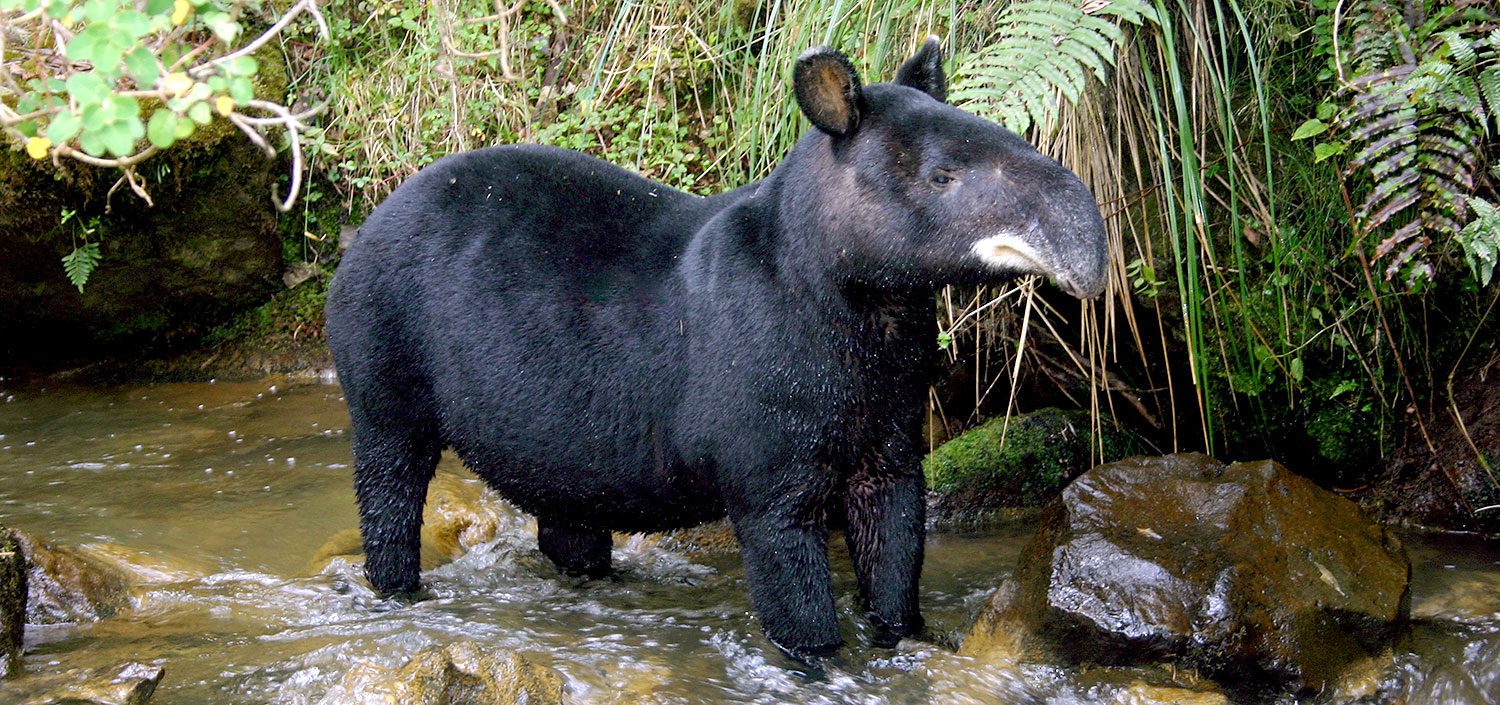
\includegraphics{images/Mountain_Tapir_large.jpg}
Mountain tapir in ``Los Nevados'' National Park. Colombia

Though it is the smallest (and furriest!) of tapir species, the Mountain tapir is the largest mammal in the tropical Andes mountain range. Their long hair is brownish to black, and their lips are lined in a white color.

The data set contains \emph{J} replicated data of detection or non-detection of the species in \emph{M} sites, taking into account that we assume that it is a closed population (`closure' assumption). This means that during the sampling there were no changes due to births, deaths, immigration or emigration. In other words, the sampling was short in time and the occurrence of species \emph{z} did not change due to demographic effects.

Clearly, we must distinguish two processes, the first is the ecological process, which generates (partially) a latent state of the occurrence \emph{z}. The second is the observation process, which produces the observed tapir detection or non-detection data. Here we assume that the observation process is governed by an imperfect detection mechanism. In other words, some tapir could have escaped my observation, which generates false negatives. We also assume that false positives are absent, meaning that anything I identify as a tapir is indeed a tapir and not a deer or a bear. To make the example more realistic, we include the effects of elevation (altitude) and forest cover on occurrence, as factors that affect occurrence linearly, decreasing it in the case of elevation, and increasing occupation linearly in the case of forest cover. In the end the two variables interact negatively with each other. These effects are introduced in the logarithmic scale occurrence as a generalized linear model (GLM) is traditionally done.

In our simulation we are going to make it explicit that it is not possible to detect all the tapirs from a sample site, so we are facing a type of error that makes us underestimate the abundance of the population. There are many reasons why we fail to spot an individual in the wild, it can be because we got distracted while the tapir passed by, because the binoculars did not have enough magnification, or simply because the tapir hid behind a tree upon smelling us, or because some other reason. In this way, we are going to register the presence (\emph{z}=1) with a probability of detection \emph{p} which we are also going to make dependent (on the logarithmic scale) of the elevation and of a co-variable that affects the detection, the temperature. In general terms, animals are more difficult to observe when the temperature is higher, and generally the higher the elevation, the lower the temperature. In this way, we assume that detection is negatively related to elevation and temperature. But it should also be noted that the negative effect on \emph{p} can also be mediated by a decrease in abundance with elevation, which also causes the probability of occupancy to decrease with elevation. Note that a co-variable, elevation affects both the ecological process (the occurrence) and the observational process (the probability of detection). This has a purpose and is likely to happen in nature many times. Occupancy models have a ``mechanistic'' basis producing a spatial variation in abundance. That is, we will have sites with greater abundance and others with less abundance. But hierarchical models, like the one we are about to build, are capable of unraveling these complex relationships between occurrence and probability of detection \citep{Kery2008, KERY2008, Kery2012}. Finally, for this first example, we are going to leave out the effect of the interaction between elevation and temperature, setting it to zero. Then we can vary this parameter to consider that effect. In summary, we are going to generate data under the following model, where the sites are indexed as \emph{i} and the repeated counts on the site are going to be referred to as \emph{j}.

\hypertarget{ecological-model}{%
\subsection{Ecological Model:}\label{ecological-model}}

\begin{equation} 
z _{i} = Bernoulli (\psi _{i})
  \label{eq:binom}
\end{equation}

\begin{equation} 
logit(\psi _{i}) = \beta _{0} + \beta _{1} \ast Elevation _{i} + \beta _{2}\ast CovForest _{i} + \beta _{3} \ast Elevation _{i} \ast CovForest _{i}
  \label{eq:binom}
\end{equation}

\hypertarget{observation-model}{%
\subsection{Observation Model:}\label{observation-model}}

\begin{equation} 
y _{ij} = Bernoulli (z _{i} * p _{ij})
  \label{eq:binom}
\end{equation}

\begin{equation} 
logit(p _{ij}) = \alpha  _{0} + \alpha  _{1} \ast Elevation _{i} + \alpha  _{2}\ast Temperature _{ij} + \alpha _{3} \ast Elevation _{i} \ast Temperature _{ij}
  \label{eq:binom}
\end{equation}

Where \(\psi\) is the occupancy and \emph{p} the probability of detection. With \(\beta\) as the regression coefficient for the occupancy covariates and \(\alpha\) the regression coefficient for the detection covariates.

We are going to generate data from the ``inside out'' and from the top down. For this, we first choose the sample size and create the values for the covariates. Second, we select the values of the ecological model parameters (the occupancy) and assemble the expected occurrence (the parameter \(\psi\), occupancy) and then obtain the random variable \emph{z} which has a Bernoulli distribution. Third, we select the values of the parameters of the observation model (the detection), to assemble the probability of detection \emph{p} and obtain the second set of a random variable \emph{y} (observed or unobserved detection of a tapir) which also has distribution Bernoulli.

To simulate the data we will use the statistical programming language R \citep{RCoreTeam2016}, which provides a wide variety of graphical and statistical modeling techniques and a large ecosystem of packages for statistical and ecological analysis. If you haven't already, download and install \href{http://www.r-project.org/}{R} on your computer, then do the same with \href{http://www.rstudio.com\%20/}{RStudio.}

\hypertarget{initial-steps-sample-size-and-covariate-values}{%
\section{Initial steps: sample size and covariate values}\label{initial-steps-sample-size-and-covariate-values}}

Start \href{http://www.rstudio.com/}{RStudio}, copy, paste and execute the commands in the gray window.

We first choose the sample size, the number of sites, and the number of repeated measures (number of visits) of presence/absence at each site.

\begin{Shaded}
\begin{Highlighting}[]
\NormalTok{M }\OtherTok{\textless{}{-}} \DecValTok{60} \CommentTok{\# Number of spatial replicas (sites)}
\NormalTok{J }\OtherTok{\textless{}{-}} \DecValTok{30} \CommentTok{\# Number of temporal replicas (repeat counts)}
\end{Highlighting}
\end{Shaded}

We then create the values for the covariates. We have elevation and forest cover as co-variables for each site. They differ from site to site but for each sampling, they are the same. While the temperature is a co-variable of the observation, so it does vary in each sampling and also in each site. Remember that the sub-index \emph{i} refers to the site and the \emph{j} to each sampling. To keep things simple our covariates are going to have a normal distribution with a mean-centered at zero and not going to extend very far on either side of zero. In real data analysis, we will have to standardize the co-variables to avoid numerical problems of difference in the scales of the co-variables and to be able to calculate the value of maximum likelihood (ML), as well as to obtain convergence in the Markov chains of the Bayesian model. Here we are going to ignore a fact of real life, and that is that the co-variables are not totally independent of each other, that is, in nature, forest cover can be related to elevation, but this is not going to be relevant, for now.

To initialize the random number generator and always get the same results we can add the following line:

\begin{Shaded}
\begin{Highlighting}[]
\FunctionTok{set.seed}\NormalTok{(}\DecValTok{24}\NormalTok{) }\CommentTok{\# Can choose seed of your choice}
\end{Highlighting}
\end{Shaded}

In this way, we can always obtain the same estimates. But then when we want to get the sampling error we will have to remove that line. For this example, we will generate values already standardized for the covariates, which are centered at zero and ranging from -1 to 1.

\begin{Shaded}
\begin{Highlighting}[]
\NormalTok{elev }\OtherTok{\textless{}{-}} \FunctionTok{runif}\NormalTok{(}\AttributeTok{n =}\NormalTok{ M, }\SpecialCharTok{{-}}\DecValTok{1}\NormalTok{, }\DecValTok{1}\NormalTok{)             }\CommentTok{\# Scaled elevation of a site}
\NormalTok{forest }\OtherTok{\textless{}{-}} \FunctionTok{runif}\NormalTok{(}\AttributeTok{n =}\NormalTok{ M, }\SpecialCharTok{{-}}\DecValTok{1}\NormalTok{, }\DecValTok{1}\NormalTok{)           }\CommentTok{\# Scaled forest cover at each site}
\NormalTok{temp }\OtherTok{\textless{}{-}} \FunctionTok{array}\NormalTok{(}\FunctionTok{runif}\NormalTok{(}\AttributeTok{n =}\NormalTok{ M}\SpecialCharTok{*}\NormalTok{J, }\SpecialCharTok{{-}}\DecValTok{1}\NormalTok{, }\DecValTok{1}\NormalTok{), }\AttributeTok{dim =} \FunctionTok{c}\NormalTok{(M, J)) }\CommentTok{\# Scaled temperature}
\end{Highlighting}
\end{Shaded}

\hypertarget{simulating-the-ecological-process-and-its-result-the-occurrence-of-the-tapir}{%
\section{Simulating the ecological process and its result: the occurrence of The Tapir}\label{simulating-the-ecological-process-and-its-result-the-occurrence-of-the-tapir}}

To simulate the occurrence of tapirs at each site, we choose the values for the parameters that govern the spatial variation in occurrence \(β_{0}\) to \(β_{3}\). The first parameter is the expected average occurrence of tapir (occupation probability) when all covariates have a value of zero, in other words the intercept of the occurrence model. We prefer to think of tapir in terms of their occurrence rather than logit (occurrence). Here we choose the occupancy intercept first and then transform it from the logarithmic scale with the logit link function.

\begin{Shaded}
\begin{Highlighting}[]
\NormalTok{mean.occupancy }\OtherTok{\textless{}{-}} \FloatTok{0.60}         \CommentTok{\# Mean expected occurrence of tapir}
\NormalTok{beta0 }\OtherTok{\textless{}{-}} \FunctionTok{plogis}\NormalTok{(mean.occupancy) }\CommentTok{\# Same on logit scale (= logit{-}scale intercept)}
\NormalTok{beta1 }\OtherTok{\textless{}{-}} \SpecialCharTok{{-}}\DecValTok{2}                    \CommentTok{\# Effect (slope) of elevation}
\NormalTok{beta2 }\OtherTok{\textless{}{-}} \DecValTok{2}                     \CommentTok{\# Effect (slope) of forest cover}
\NormalTok{beta3 }\OtherTok{\textless{}{-}} \DecValTok{1}                     \CommentTok{\# Interaction effect (slope) of elev and forest}
\end{Highlighting}
\end{Shaded}

Here we apply the linear model (to the logarithmic scale) and obtain the logit transformation of the occupancy probability, which we invert with the logit transformation to obtain the tapir occupancy and plot everything.

\begin{Shaded}
\begin{Highlighting}[]
\NormalTok{logit.psi }\OtherTok{\textless{}{-}}\NormalTok{ beta0 }\SpecialCharTok{+}\NormalTok{ beta1 }\SpecialCharTok{*}\NormalTok{ elev }\SpecialCharTok{+}\NormalTok{ beta2 }\SpecialCharTok{*}\NormalTok{ forest }\SpecialCharTok{+}\NormalTok{ beta3 }\SpecialCharTok{*}\NormalTok{ elev }\SpecialCharTok{*}\NormalTok{ forest}
\NormalTok{psi }\OtherTok{\textless{}{-}} \FunctionTok{plogis}\NormalTok{(logit.psi)      }\CommentTok{\# Inverse link transformation}

\CommentTok{\# par()              \# view current settings}
\NormalTok{opar }\OtherTok{\textless{}{-}} \FunctionTok{par}\NormalTok{()      }\CommentTok{\# make a copy of current settings}
\FunctionTok{par}\NormalTok{(}\AttributeTok{mfrow =} \FunctionTok{c}\NormalTok{(}\DecValTok{2}\NormalTok{, }\DecValTok{2}\NormalTok{), }\AttributeTok{mar =} \FunctionTok{c}\NormalTok{(}\DecValTok{5}\NormalTok{,}\DecValTok{4}\NormalTok{,}\DecValTok{2}\NormalTok{,}\DecValTok{2}\NormalTok{), }\AttributeTok{cex.main =} \DecValTok{1}\NormalTok{)}
\FunctionTok{curve}\NormalTok{(}\FunctionTok{plogis}\NormalTok{(beta0 }\SpecialCharTok{+}\NormalTok{ beta1}\SpecialCharTok{*}\NormalTok{x), }\SpecialCharTok{{-}}\DecValTok{1}\NormalTok{, }\DecValTok{1}\NormalTok{, }\AttributeTok{col =} \StringTok{"red"}\NormalTok{, }\AttributeTok{frame.plot =} \ConstantTok{FALSE}\NormalTok{, }\AttributeTok{ylim =} \FunctionTok{c}\NormalTok{(}\DecValTok{0}\NormalTok{, }\DecValTok{1}\NormalTok{),}
      \AttributeTok{xlab =} \StringTok{"Altitud"}\NormalTok{, }\AttributeTok{ylab =} \StringTok{"psi"}\NormalTok{, }\AttributeTok{lwd =} \DecValTok{2}\NormalTok{)}
\FunctionTok{text}\NormalTok{(}\FloatTok{0.9}\NormalTok{, }\FloatTok{0.95}\NormalTok{, }\StringTok{"A"}\NormalTok{, }\AttributeTok{cex =} \FloatTok{1.5}\NormalTok{)}
\FunctionTok{plot}\NormalTok{(elev, psi, }\AttributeTok{frame.plot =} \ConstantTok{FALSE}\NormalTok{, }\AttributeTok{ylim =} \FunctionTok{c}\NormalTok{(}\DecValTok{0}\NormalTok{, }\DecValTok{1}\NormalTok{), }\AttributeTok{xlab =} \StringTok{"Altitud"}\NormalTok{, }\AttributeTok{ylab =} \StringTok{""}\NormalTok{)}
\FunctionTok{text}\NormalTok{(}\FloatTok{0.9}\NormalTok{, }\FloatTok{0.95}\NormalTok{, }\StringTok{"B"}\NormalTok{, }\AttributeTok{cex =} \FloatTok{1.5}\NormalTok{)}
\FunctionTok{curve}\NormalTok{(}\FunctionTok{plogis}\NormalTok{(beta0 }\SpecialCharTok{+}\NormalTok{ beta2}\SpecialCharTok{*}\NormalTok{x), }\SpecialCharTok{{-}}\DecValTok{1}\NormalTok{, }\DecValTok{1}\NormalTok{, }\AttributeTok{col =} \StringTok{"red"}\NormalTok{, }\AttributeTok{frame.plot =} \ConstantTok{FALSE}\NormalTok{, }\AttributeTok{ylim =} \FunctionTok{c}\NormalTok{(}\DecValTok{0}\NormalTok{, }\DecValTok{1}\NormalTok{), }
      \AttributeTok{xlab =} \StringTok{"Forest cover"}\NormalTok{, }\AttributeTok{ylab =} \StringTok{"psi"}\NormalTok{, }\AttributeTok{lwd =} \DecValTok{2}\NormalTok{)}
\FunctionTok{text}\NormalTok{(}\SpecialCharTok{{-}}\FloatTok{0.9}\NormalTok{, }\FloatTok{0.95}\NormalTok{, }\StringTok{"C"}\NormalTok{, }\AttributeTok{cex =} \FloatTok{1.5}\NormalTok{)}
\FunctionTok{plot}\NormalTok{(forest, psi, }\AttributeTok{frame.plot =} \ConstantTok{FALSE}\NormalTok{, }\AttributeTok{ylim =} \FunctionTok{c}\NormalTok{(}\DecValTok{0}\NormalTok{, }\DecValTok{1}\NormalTok{), }\AttributeTok{xlab =} \StringTok{"Forest cover"}\NormalTok{, }\AttributeTok{ylab =} \StringTok{""}\NormalTok{)}
\FunctionTok{text}\NormalTok{(}\SpecialCharTok{{-}}\FloatTok{0.9}\NormalTok{, }\FloatTok{0.95}\NormalTok{, }\StringTok{"D"}\NormalTok{, }\AttributeTok{cex =} \FloatTok{1.5}\NormalTok{)}
\end{Highlighting}
\end{Shaded}

\begin{figure}
\centering
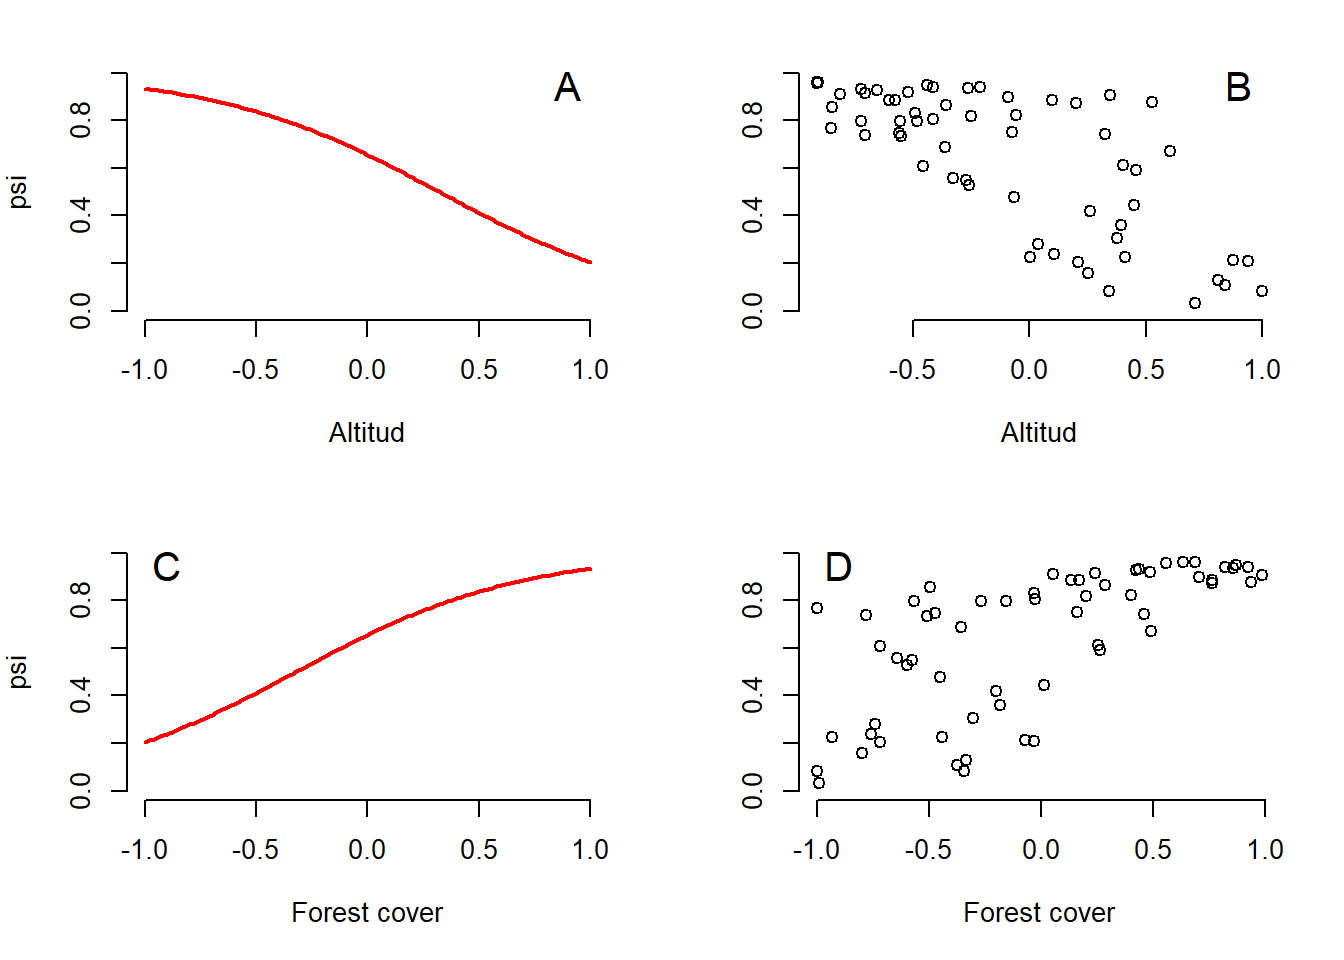
\includegraphics{Occu_Book_files/figure-latex/fig2-1.pdf}
\caption{\label{fig:fig2}Two ways to show the relationship between the probability of occurrence of tapir and the covariates. (A) Relationship between psi and elevation for a constant value (mean equal to zero) of forest cover. (B) Relationship between psi and elevation in an observed value of forest cover. (C) Forest cover psi ratio for a constant elevation (at mean zero). (D) Relationship psi forest cover for the observed value of elevation.}
\end{figure}

\begin{Shaded}
\begin{Highlighting}[]
\CommentTok{\# dev.off()}
\FunctionTok{par}\NormalTok{(opar)          }\CommentTok{\# restore original par settings}
\end{Highlighting}
\end{Shaded}

To better show the joint relationship between the two covariates and psi, we need to make a surface plot. Here we have not changed anything about the simulation, we have only added more data to it to better visualize it.

\begin{Shaded}
\begin{Highlighting}[]
\CommentTok{\# Compute expected occurrence for a grid of elevation and forest cover}
\NormalTok{cov1 }\OtherTok{\textless{}{-}} \FunctionTok{seq}\NormalTok{(}\SpecialCharTok{{-}}\DecValTok{1}\NormalTok{, }\DecValTok{1}\NormalTok{, , }\DecValTok{100}\NormalTok{)                       }\CommentTok{\# Values for elevation}
\NormalTok{cov2 }\OtherTok{\textless{}{-}} \FunctionTok{seq}\NormalTok{(}\SpecialCharTok{{-}}\DecValTok{1}\NormalTok{, }\DecValTok{1}\NormalTok{, , }\DecValTok{100}\NormalTok{)                       }\CommentTok{\# Values for forest cover}
\NormalTok{psi.matrix }\OtherTok{\textless{}{-}} \FunctionTok{array}\NormalTok{(}\ConstantTok{NA}\NormalTok{, }\AttributeTok{dim =} \FunctionTok{c}\NormalTok{(}\DecValTok{100}\NormalTok{, }\DecValTok{100}\NormalTok{))      }\CommentTok{\# Prediction matrix, for every }
\CommentTok{\# combination of values of elevation and forest cover}

\ControlFlowTok{for}\NormalTok{(i }\ControlFlowTok{in} \DecValTok{1}\SpecialCharTok{:}\DecValTok{100}\NormalTok{)\{}
   \ControlFlowTok{for}\NormalTok{(j }\ControlFlowTok{in} \DecValTok{1}\SpecialCharTok{:}\DecValTok{100}\NormalTok{)\{}
\NormalTok{      psi.matrix[i, j] }\OtherTok{\textless{}{-}} \FunctionTok{plogis}\NormalTok{(beta0 }\SpecialCharTok{+} 
\NormalTok{                                   beta1 }\SpecialCharTok{*}\NormalTok{ cov1[i] }\SpecialCharTok{+} 
\NormalTok{                                   beta2 }\SpecialCharTok{*}\NormalTok{ cov2[j] }\SpecialCharTok{+} 
\NormalTok{                                   beta3 }\SpecialCharTok{*}\NormalTok{ cov1[i] }\SpecialCharTok{*}\NormalTok{ cov2[j] )}
\NormalTok{   \}}
\NormalTok{\}}

\NormalTok{mapPalette }\OtherTok{\textless{}{-}} \FunctionTok{colorRampPalette}\NormalTok{(}\FunctionTok{c}\NormalTok{(}\StringTok{"grey"}\NormalTok{, }\StringTok{"yellow"}\NormalTok{, }\StringTok{"orange"}\NormalTok{, }\StringTok{"red"}\NormalTok{))}
\FunctionTok{image}\NormalTok{(}\AttributeTok{x =}\NormalTok{ cov1, }\AttributeTok{y =}\NormalTok{ cov2, }\AttributeTok{z =}\NormalTok{ psi.matrix, }\AttributeTok{col =} \FunctionTok{mapPalette}\NormalTok{(}\DecValTok{100}\NormalTok{), }\AttributeTok{xlab =} \StringTok{"Altitud"}\NormalTok{, }
      \AttributeTok{ylab =} \StringTok{"Forest cover"}\NormalTok{, }\AttributeTok{cex.lab =} \FloatTok{1.2}\NormalTok{)}
\FunctionTok{contour}\NormalTok{(}\AttributeTok{x =}\NormalTok{ cov1, }\AttributeTok{y =}\NormalTok{ cov2, }\AttributeTok{z =}\NormalTok{ psi.matrix, }\AttributeTok{add =} \ConstantTok{TRUE}\NormalTok{, }\AttributeTok{lwd =} \DecValTok{1}\NormalTok{)}
\FunctionTok{matpoints}\NormalTok{(elev, forest, }\AttributeTok{pch=}\StringTok{"+"}\NormalTok{, }\AttributeTok{cex=}\FloatTok{0.8}\NormalTok{)}
\end{Highlighting}
\end{Shaded}

\begin{figure}
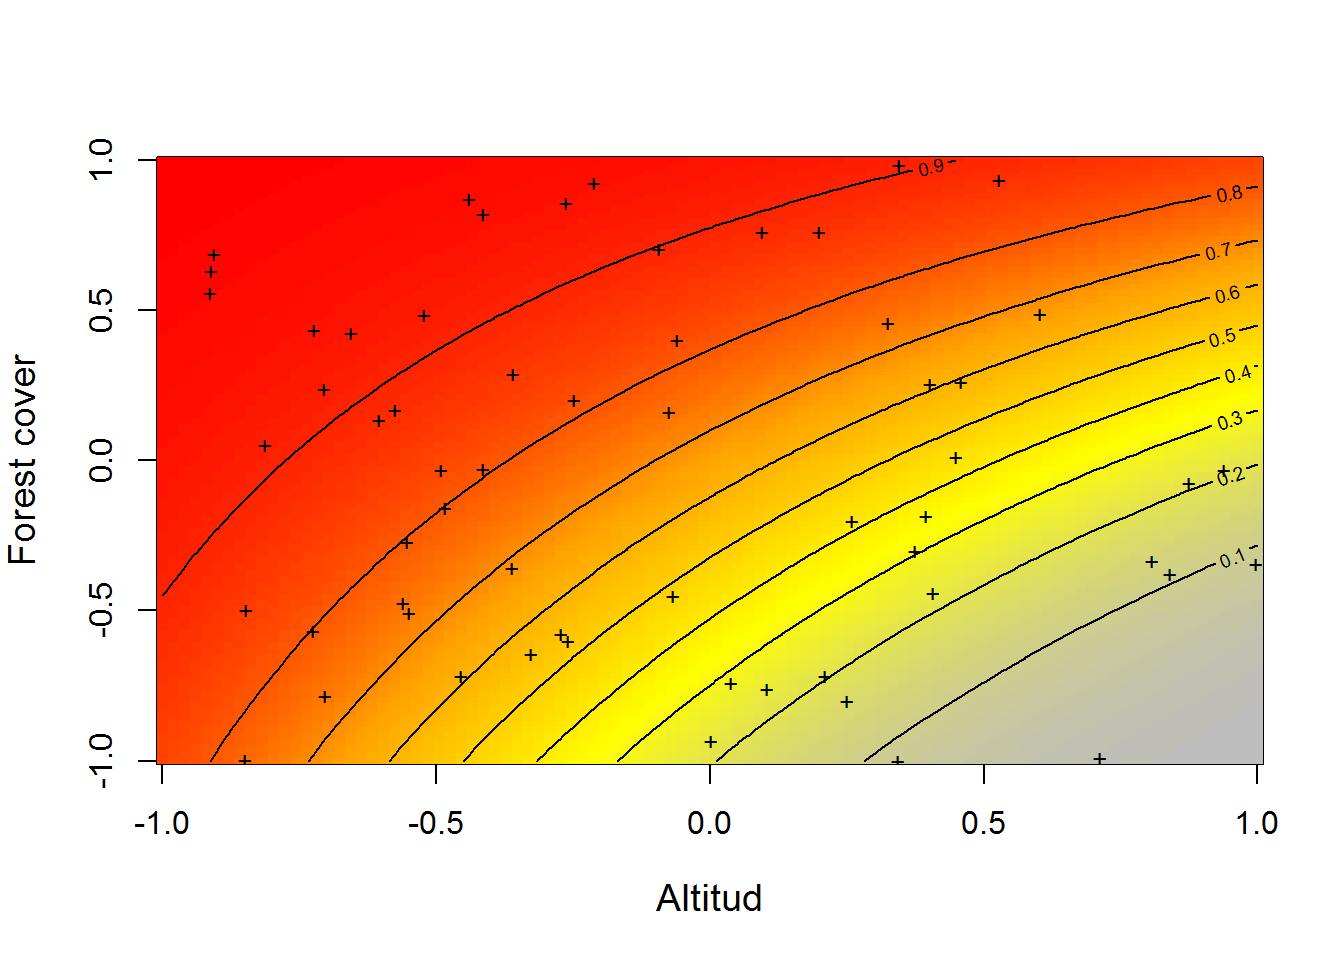
\includegraphics{Occu_Book_files/figure-latex/fig3-1} \caption[fig3]{Relationship constructed between the simulated data of the expected occurrence (occupation) of tapir (psi) represented with the color scale from gray to red, against elevation and forest cover simultaneously. In this case the interaction between the two covariates is given by the value of beta3 = 1 that we have established previously.}\label{fig:fig3}
\end{figure}

So far we have not introduced any stochastic variation in the relationship between tapir occurrence and covariates. To do this we must make use of some statistical models, or statistical distributions, to describe the random variability around the expected value of psi. The typical way to introduce this random variation is to obtain the occurrence of tapir at each site \emph{i}, \(z _{i}\) , from a Bernoulli distribution with the expected values (\(\psi _{i}\)).

\hypertarget{why-bernoulli}{%
\subsection{Why Bernoulli?}\label{why-bernoulli}}

In the ecological process \(z _{i}\) tapir occurrence is represented by a Bernoulli-type distribution where tapir is present at a site represented as the occupancy \(\psi\) at a site where it is present, or not present 1-\(\psi\). The Bernoulli distribution is a special case of the binomial distribution, and its best example is a single toss of a coin. If you require a more extensive, basic, detailed explanation and with more examples, I recommend you visit \href{https://www.khanacademy.org/math/statistics-probability/random-variables-stats-library/binomial-mean-standard-dev-formulas/v/mean-and-variance-of-bernoulli-distribution-example}{khanacademy.}

\begin{Shaded}
\begin{Highlighting}[]
\NormalTok{z }\OtherTok{\textless{}{-}} \FunctionTok{rbinom}\NormalTok{(}\AttributeTok{n =}\NormalTok{ M, }\AttributeTok{size =} \DecValTok{1}\NormalTok{, }\AttributeTok{prob =}\NormalTok{ psi)  }\CommentTok{\# Realised occurrence. A Bernoulli}
\FunctionTok{sum}\NormalTok{(z)                                    }\CommentTok{\# Total number of occupied sites}
\end{Highlighting}
\end{Shaded}

\begin{verbatim}
## [1] 40
\end{verbatim}

\begin{Shaded}
\begin{Highlighting}[]
\FunctionTok{table}\NormalTok{(z)                                  }\CommentTok{\# Frequency distribution of tapir occurrence}
\end{Highlighting}
\end{Shaded}

\begin{verbatim}
## z
##  0  1 
## 20 40
\end{verbatim}

Here we have created the result of the ecological process: site-specific occurrence \(z _{1}\). We see that 20 sites are not occupied and the remaining 40 sites are occupied

\hypertarget{simulating-the-observation-process-and-its-result-the-detection}{%
\section{Simulating the observation process and its result: the detection}\label{simulating-the-observation-process-and-its-result-the-detection}}

Occurrence \emph{z} is not what we normally see, as there is a chance that we will fail to observe an individual. Hence there is a binary measure of error when we measure occurrence (we observe it or we don't observe it). We assume that we can make only one of the two possible sightings (yes, no), but we may have missed a tapir sighting somewhere, so the probability of detection is less than one, and the error measure is affected by coverage. of forest and temperature. Keep in mind that we will never register the presence of a tapir when in fact there are no tapir. In other words, we are assuming that we have no false positives. To make it explicit that we have an interaction effect between two covariates in our data, we are going to allow an interaction effect in the code, but set it to zero and thus have no effect in the model that generates the data. We first select the values for \(\alpha _{0}\) to \(\alpha _{3}\), where the first is the probability of detection for the tapir, on the logit scale, when all detection covariates have a value of zero. We have chosen the intercept of the detection model and then transformed it with the plogis link function. This is not the same as the average detection probability, which is higher in our simulation model, as we will see later.

\begin{Shaded}
\begin{Highlighting}[]
\NormalTok{mean.detection }\OtherTok{\textless{}{-}} \FloatTok{0.3}            \CommentTok{\# Mean expected detection}
\NormalTok{alpha0 }\OtherTok{\textless{}{-}} \FunctionTok{qlogis}\NormalTok{(mean.detection) }\CommentTok{\# same on logit scale (intercept)}
\NormalTok{alpha1 }\OtherTok{\textless{}{-}} \SpecialCharTok{{-}}\DecValTok{1}                     \CommentTok{\# Effect (slope) of elevation}
\NormalTok{alpha2 }\OtherTok{\textless{}{-}} \SpecialCharTok{{-}}\DecValTok{3}                     \CommentTok{\# Effect (slope) of temperature}
\NormalTok{alpha3 }\OtherTok{\textless{}{-}} \DecValTok{0}                      \CommentTok{\# Interaction effect (slope) of elevevation and temperature}
\end{Highlighting}
\end{Shaded}

Applying the linear model, we have the logit of the detection probability of the tapir for each site and sampling, and applying the inverse transformation (plogis), we obtain a matrix of dimensions 60 by 30 with the probability of detection for each site \emph{i} and sampling \emph{j}. Finally, we plot the relationships for the probability of detection in the data.

\begin{Shaded}
\begin{Highlighting}[]
\NormalTok{logit.p }\OtherTok{\textless{}{-}}\NormalTok{ alpha0 }\SpecialCharTok{+}\NormalTok{ alpha1 }\SpecialCharTok{*}\NormalTok{ elev }\SpecialCharTok{+}\NormalTok{ alpha2 }\SpecialCharTok{*}\NormalTok{ temp }\SpecialCharTok{+}\NormalTok{ alpha3 }\SpecialCharTok{*}\NormalTok{ elev }\SpecialCharTok{*}\NormalTok{ temp}
\NormalTok{p }\OtherTok{\textless{}{-}} \FunctionTok{plogis}\NormalTok{(logit.p)             }\CommentTok{\# Inverse link transform }
\FunctionTok{mean}\NormalTok{(p)                          }\CommentTok{\# average per{-}site p is about 0.39}
\end{Highlighting}
\end{Shaded}

\begin{verbatim}
## [1] 0.3928068
\end{verbatim}

\begin{Shaded}
\begin{Highlighting}[]
\FunctionTok{par}\NormalTok{(}\AttributeTok{mfrow =} \FunctionTok{c}\NormalTok{(}\DecValTok{2}\NormalTok{, }\DecValTok{2}\NormalTok{), }\AttributeTok{mar =} \FunctionTok{c}\NormalTok{(}\DecValTok{5}\NormalTok{,}\DecValTok{4}\NormalTok{,}\DecValTok{2}\NormalTok{,}\DecValTok{2}\NormalTok{), }\AttributeTok{cex.main =} \DecValTok{1}\NormalTok{)}
\FunctionTok{curve}\NormalTok{(}\FunctionTok{plogis}\NormalTok{(alpha0 }\SpecialCharTok{+}\NormalTok{ alpha1}\SpecialCharTok{*}\NormalTok{x), }\SpecialCharTok{{-}}\DecValTok{1}\NormalTok{, }\DecValTok{1}\NormalTok{, }\AttributeTok{col =} \StringTok{"red"}\NormalTok{, }\AttributeTok{frame.plot =} \ConstantTok{FALSE}\NormalTok{, }\AttributeTok{ylim =} \FunctionTok{c}\NormalTok{(}\DecValTok{0}\NormalTok{, }\FloatTok{1.1}\NormalTok{), }
      \AttributeTok{xlab =} \StringTok{"Altitud"}\NormalTok{, }\AttributeTok{ylab =} \StringTok{"p"}\NormalTok{, }\AttributeTok{lwd =} \DecValTok{2}\NormalTok{)}
\FunctionTok{text}\NormalTok{(}\SpecialCharTok{{-}}\FloatTok{0.9}\NormalTok{, }\FloatTok{1.05}\NormalTok{, }\StringTok{"A"}\NormalTok{, }\AttributeTok{cex =} \FloatTok{1.5}\NormalTok{)}
\FunctionTok{matplot}\NormalTok{(elev, p, }\AttributeTok{pch =} \StringTok{"*"}\NormalTok{, }\AttributeTok{frame.plot =} \ConstantTok{FALSE}\NormalTok{, }\AttributeTok{ylim =} \FunctionTok{c}\NormalTok{(}\DecValTok{0}\NormalTok{, }\FloatTok{1.1}\NormalTok{), }\AttributeTok{xlab =} \StringTok{"Altitud"}\NormalTok{, }
        \AttributeTok{ylab =} \StringTok{""}\NormalTok{)}
\FunctionTok{text}\NormalTok{(}\SpecialCharTok{{-}}\FloatTok{0.9}\NormalTok{, }\FloatTok{1.05}\NormalTok{, }\StringTok{"B"}\NormalTok{, }\AttributeTok{cex =} \FloatTok{1.5}\NormalTok{)}
\FunctionTok{curve}\NormalTok{(}\FunctionTok{plogis}\NormalTok{(alpha0 }\SpecialCharTok{+}\NormalTok{ alpha2}\SpecialCharTok{*}\NormalTok{x), }\SpecialCharTok{{-}}\DecValTok{1}\NormalTok{, }\DecValTok{1}\NormalTok{, }\AttributeTok{col =} \StringTok{"red"}\NormalTok{, }\AttributeTok{frame.plot =} \ConstantTok{FALSE}\NormalTok{, }\AttributeTok{ylim =} \FunctionTok{c}\NormalTok{(}\DecValTok{0}\NormalTok{, }\FloatTok{1.1}\NormalTok{), }
      \AttributeTok{xlab =} \StringTok{"Temperature"}\NormalTok{, }\AttributeTok{ylab =} \StringTok{"p"}\NormalTok{, }\AttributeTok{lwd =} \DecValTok{2}\NormalTok{)}
\FunctionTok{text}\NormalTok{(}\SpecialCharTok{{-}}\FloatTok{0.9}\NormalTok{, }\FloatTok{1.05}\NormalTok{, }\StringTok{"C"}\NormalTok{, }\AttributeTok{cex =} \FloatTok{1.5}\NormalTok{)}
\FunctionTok{matplot}\NormalTok{(temp, p, }\AttributeTok{pch =} \StringTok{"*"}\NormalTok{, }\AttributeTok{frame.plot =} \ConstantTok{FALSE}\NormalTok{, }\AttributeTok{ylim =} \FunctionTok{c}\NormalTok{(}\DecValTok{0}\NormalTok{, }\FloatTok{1.1}\NormalTok{), }\AttributeTok{xlab =} \StringTok{"Temperature"}\NormalTok{, }
        \AttributeTok{ylab =} \StringTok{"p"}\NormalTok{)}
\FunctionTok{text}\NormalTok{(}\SpecialCharTok{{-}}\FloatTok{0.9}\NormalTok{, }\FloatTok{1.05}\NormalTok{, }\StringTok{"D"}\NormalTok{, }\AttributeTok{cex =} \FloatTok{1.5}\NormalTok{)}
\end{Highlighting}
\end{Shaded}

\begin{figure}
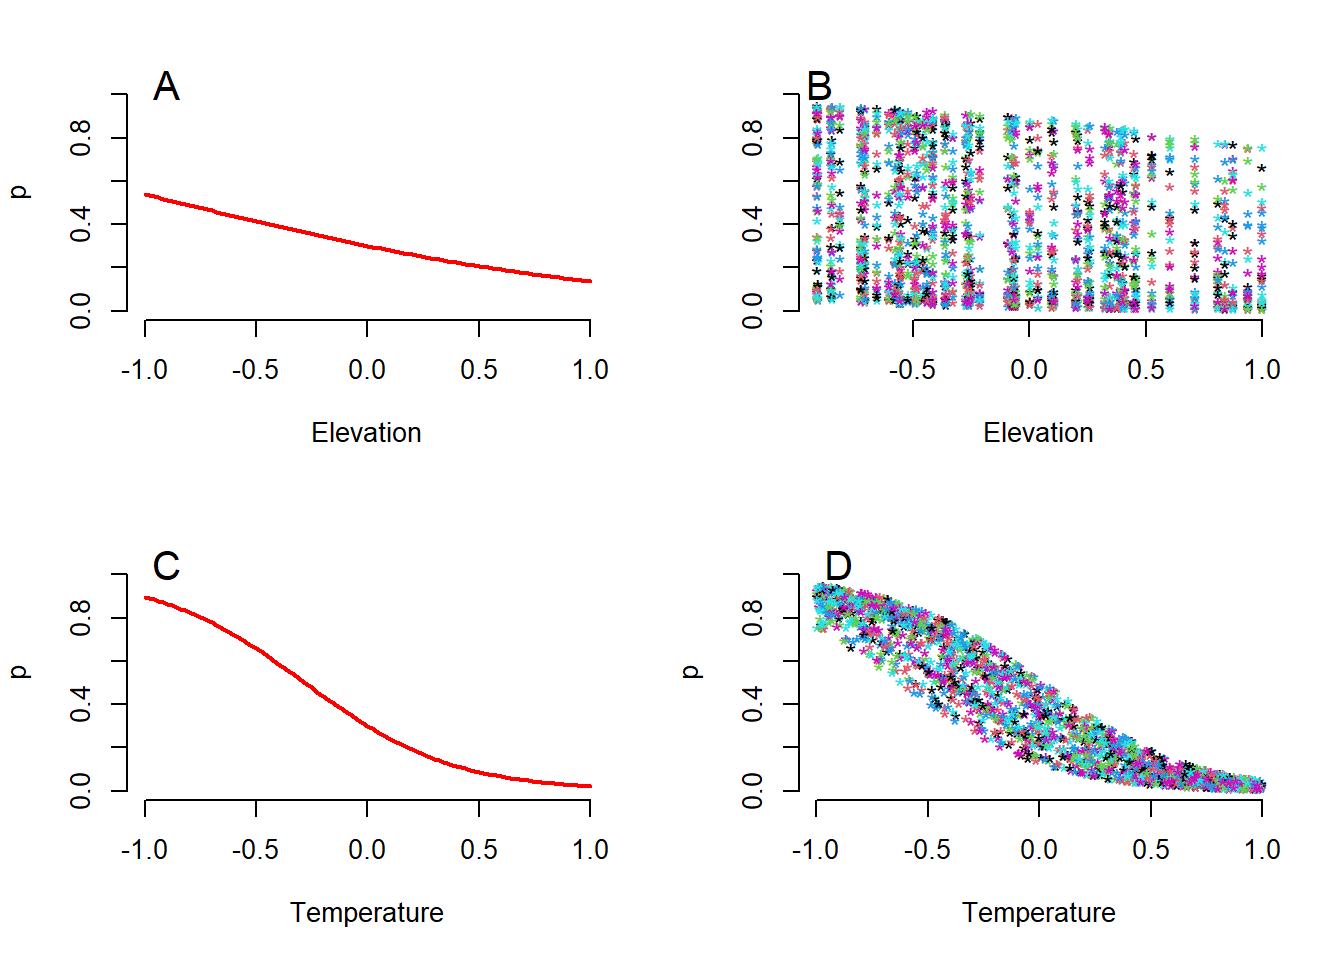
\includegraphics{Occu_Book_files/figure-latex/fig4-1} \caption[fig4]{Two ways to show the relationships between the expected detection probability of the tapir (_p_) and the two variables elevation and temperature. (A) Relationship _p_ and elevation for constant temperature (at the mean value, which is equal to zero). (B) Relationship between _p_ and elevation in the observed value of temperature quantity. (C) Relationship between _p_ and temperature for a constant value of elevation (at mean elevation equal to zero). (D) Relationship between _p_ and temperature for an observed value of elevation.}\label{fig:fig4}
\end{figure}

In a similar way we are going to produce a graph of a surface with the joint relationship between elevation, temperature and the probability of detection of the tapir (\emph{p}), acting simultaneously. The relationship on the logarithmic scale is represented by a sloped plane that represents the interaction between elevation and forest cover.

\begin{Shaded}
\begin{Highlighting}[]
\CommentTok{\# Compute expected detection probability for a grid of elevation and temperature}
\NormalTok{cov1 }\OtherTok{\textless{}{-}} \FunctionTok{seq}\NormalTok{(}\SpecialCharTok{{-}}\DecValTok{1}\NormalTok{, }\DecValTok{1}\NormalTok{,,}\DecValTok{100}\NormalTok{)                  }\CommentTok{\# Values of elevation}
\NormalTok{cov2 }\OtherTok{\textless{}{-}} \FunctionTok{seq}\NormalTok{(}\SpecialCharTok{{-}}\DecValTok{1}\NormalTok{,}\DecValTok{1}\NormalTok{,,}\DecValTok{100}\NormalTok{)                   }\CommentTok{\# Values of temperature}
\NormalTok{p.matrix }\OtherTok{\textless{}{-}} \FunctionTok{array}\NormalTok{(}\ConstantTok{NA}\NormalTok{, }\AttributeTok{dim =} \FunctionTok{c}\NormalTok{(}\DecValTok{100}\NormalTok{, }\DecValTok{100}\NormalTok{)) }\CommentTok{\# Prediction matrix which combines }
\CommentTok{\# every value in cov 1 with every other in cov2}
\ControlFlowTok{for}\NormalTok{(i }\ControlFlowTok{in} \DecValTok{1}\SpecialCharTok{:}\DecValTok{100}\NormalTok{)\{}
   \ControlFlowTok{for}\NormalTok{(j }\ControlFlowTok{in} \DecValTok{1}\SpecialCharTok{:}\DecValTok{100}\NormalTok{)\{}
\NormalTok{      p.matrix[i, j] }\OtherTok{\textless{}{-}} \FunctionTok{plogis}\NormalTok{(alpha0 }\SpecialCharTok{+}\NormalTok{ alpha1 }\SpecialCharTok{*}\NormalTok{ cov1[i] }\SpecialCharTok{+} 
\NormalTok{                                 alpha2 }\SpecialCharTok{*}\NormalTok{ cov2[j] }\SpecialCharTok{+} 
\NormalTok{                                 alpha3 }\SpecialCharTok{*}\NormalTok{ cov1[i] }\SpecialCharTok{*}\NormalTok{ cov2[j])}
\NormalTok{   \}}
\NormalTok{\}}
\FunctionTok{image}\NormalTok{(}\AttributeTok{x =}\NormalTok{ cov1, }\AttributeTok{y =}\NormalTok{ cov2, }\AttributeTok{z =}\NormalTok{ p.matrix, }\AttributeTok{col =} \FunctionTok{mapPalette}\NormalTok{(}\DecValTok{100}\NormalTok{), }\AttributeTok{xlab =} \StringTok{"Altitud"}\NormalTok{, }
      \AttributeTok{ylab =} \StringTok{"Temperature"}\NormalTok{, }\AttributeTok{cex.lab =} \FloatTok{1.2}\NormalTok{)}
\FunctionTok{contour}\NormalTok{(}\AttributeTok{x =}\NormalTok{ cov1, }\AttributeTok{y =}\NormalTok{ cov2, }\AttributeTok{z =}\NormalTok{ p.matrix, }\AttributeTok{add =} \ConstantTok{TRUE}\NormalTok{, }\AttributeTok{lwd =} \DecValTok{1}\NormalTok{)}
\FunctionTok{matpoints}\NormalTok{(elev, temp, }\AttributeTok{pch=}\StringTok{"+"}\NormalTok{, }\AttributeTok{cex=}\FloatTok{0.7}\NormalTok{, }\AttributeTok{col =} \StringTok{"black"}\NormalTok{)}
\end{Highlighting}
\end{Shaded}

\begin{figure}
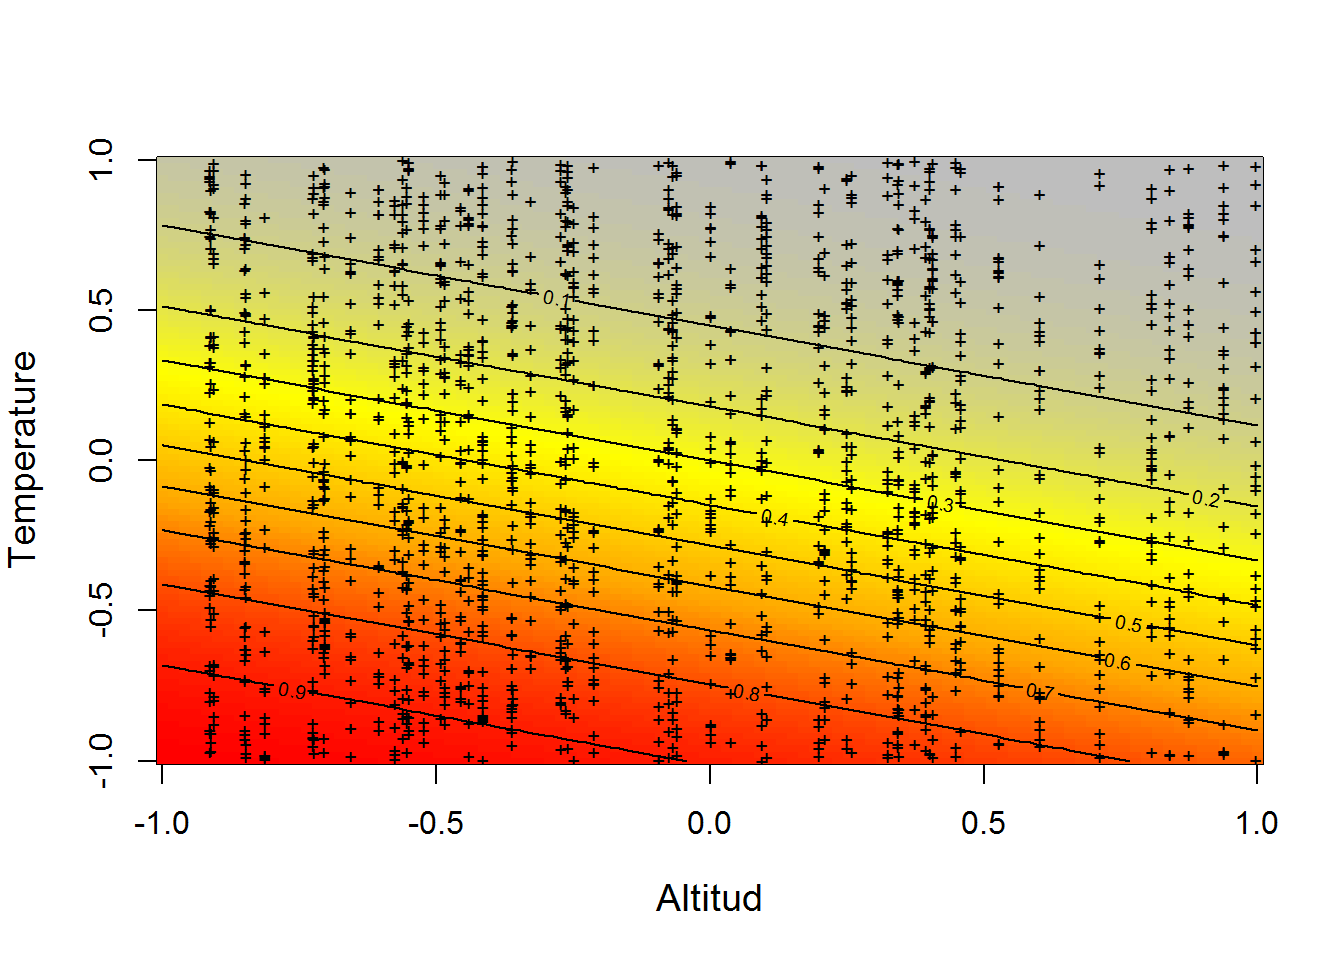
\includegraphics{Occu_Book_files/figure-latex/fig5-1} \caption[fig5]{Relationship constructed between the simulated data of the expected probability of detection (detectability) of tapir (p) represented with the color scale from gray to red, against elevation and temperature simultaneously. In this case, the interaction between the two covariates has a linear relationship that is given by the value of alpha3 = 0 that we have previously established.}\label{fig:fig5}
\end{figure}

So far we have modeled the two processes, the ecological \(z\) and the observation process \emph{p} separately. Now we will have to put them together, and for this we multiply the result of the ecological process by the probability of detection within a Bernoulli distribution.

\hypertarget{uniting-the-two-processes-the-ecological-and-the-observation}{%
\subsection{Uniting the two processes the ecological and the observation}\label{uniting-the-two-processes-the-ecological-and-the-observation}}

When we ``measure'' the occurrence, the imperfect detection represents a source of error with a Bernoulli-type distribution (for example, the presence of the deer in a place where it is detected with a probability \emph{p}, or it is not detected as 1-\emph{p}) . By applying this observation process we produce repeated measures of the presence or absence (1 or 0) of deer at each site. Remember that the Bernoulli distribution is a special case of the binomial distribution, and its best example is a single coin toss.

Right now we are establishing the hierarchy in the hierarchical model. Here we are nesting the ecological process ``within'' the observation process.

\begin{Shaded}
\begin{Highlighting}[]
\NormalTok{y }\OtherTok{\textless{}{-}} \FunctionTok{matrix}\NormalTok{(}\ConstantTok{NA}\NormalTok{, }\AttributeTok{nrow =}\NormalTok{ M, }\AttributeTok{ncol =}\NormalTok{ J)      }\CommentTok{\# Prepare array for counts}
\ControlFlowTok{for}\NormalTok{ (i }\ControlFlowTok{in} \DecValTok{1}\SpecialCharTok{:}\NormalTok{J)\{                          }\CommentTok{\# Generate counts}
\NormalTok{   y[,i] }\OtherTok{\textless{}{-}} \FunctionTok{rbinom}\NormalTok{(}\AttributeTok{n =}\NormalTok{ M, }\AttributeTok{size =} \DecValTok{1}\NormalTok{, }\AttributeTok{prob =}\NormalTok{ z}\SpecialCharTok{*}\NormalTok{p[,i])   }\CommentTok{\# this is the Bernoulli}
\NormalTok{\}}
\end{Highlighting}
\end{Shaded}

So far we have simulated the presence/absence of mountain tapirs at 60 sites during 30 sampling sessions. Let's see what the tables contain. Remember that the sites are in the rows and the repeated samples in the columns. For comparison, we will show the true occurrence in the first column for 30 sites and only five samples.

\begin{Shaded}
\begin{Highlighting}[]
\FunctionTok{library}\NormalTok{(knitr)}
\FunctionTok{kable}\NormalTok{(}\FunctionTok{as.data.frame}\NormalTok{(}\FunctionTok{head}\NormalTok{(}\FunctionTok{cbind}\NormalTok{(}\StringTok{"True Presence/Absence"} \OtherTok{=}\NormalTok{ z, }
           \StringTok{"1st survey"} \OtherTok{=}\NormalTok{ y[,}\DecValTok{1}\NormalTok{], }
           \StringTok{"2nd survey"} \OtherTok{=}\NormalTok{ y[,}\DecValTok{2}\NormalTok{], }
           \StringTok{"3rd survey"} \OtherTok{=}\NormalTok{ y[,}\DecValTok{3}\NormalTok{],}
           \StringTok{"4th survey"} \OtherTok{=}\NormalTok{ y[,}\DecValTok{4}\NormalTok{],}
           \StringTok{"5th survey"} \OtherTok{=}\NormalTok{ y[,}\DecValTok{5}\NormalTok{]), }\DecValTok{30}\NormalTok{)) )   }\CommentTok{\# First 30 rows (= sites)}
\end{Highlighting}
\end{Shaded}

\begin{tabular}{r|r|r|r|r|r}
\hline
True Presence/Absence & 1st survey & 2nd survey & 3rd survey & 4th survey & 5th survey\\
\hline
1 & 0 & 1 & 0 & 1 & 0\\
\hline
1 & 0 & 0 & 0 & 1 & 1\\
\hline
1 & 0 & 1 & 0 & 1 & 0\\
\hline
0 & 0 & 0 & 0 & 0 & 0\\
\hline
1 & 1 & 1 & 1 & 0 & 0\\
\hline
1 & 0 & 1 & 0 & 0 & 0\\
\hline
1 & 0 & 0 & 1 & 0 & 1\\
\hline
0 & 0 & 0 & 0 & 0 & 0\\
\hline
1 & 0 & 0 & 0 & 1 & 1\\
\hline
1 & 1 & 0 & 0 & 0 & 0\\
\hline
0 & 0 & 0 & 0 & 0 & 0\\
\hline
0 & 0 & 0 & 0 & 0 & 0\\
\hline
0 & 0 & 0 & 0 & 0 & 0\\
\hline
1 & 0 & 0 & 0 & 0 & 0\\
\hline
1 & 1 & 0 & 0 & 0 & 0\\
\hline
0 & 0 & 0 & 0 & 0 & 0\\
\hline
1 & 0 & 0 & 1 & 1 & 0\\
\hline
1 & 1 & 1 & 1 & 1 & 0\\
\hline
0 & 0 & 0 & 0 & 0 & 0\\
\hline
1 & 0 & 0 & 0 & 1 & 1\\
\hline
1 & 1 & 1 & 1 & 1 & 0\\
\hline
0 & 0 & 0 & 0 & 0 & 0\\
\hline
0 & 0 & 0 & 0 & 0 & 0\\
\hline
1 & 1 & 0 & 0 & 0 & 1\\
\hline
1 & 0 & 0 & 0 & 1 & 1\\
\hline
0 & 0 & 0 & 0 & 0 & 0\\
\hline
1 & 1 & 1 & 0 & 1 & 0\\
\hline
1 & 0 & 1 & 1 & 0 & 0\\
\hline
1 & 1 & 1 & 0 & 0 & 0\\
\hline
1 & 0 & 1 & 0 & 0 & 1\\
\hline
\end{tabular}

Now we will finally visualize graphically the data of ones and zeros that we have simulated for our sampling. Remember that these are values of ones that represent whether or not we have detected the tapir at each of the sampling sites on each of the visits.

\begin{Shaded}
\begin{Highlighting}[]
\FunctionTok{par}\NormalTok{(}\AttributeTok{mfrow =} \FunctionTok{c}\NormalTok{(}\DecValTok{2}\NormalTok{, }\DecValTok{2}\NormalTok{), }\AttributeTok{mar =} \FunctionTok{c}\NormalTok{(}\DecValTok{5}\NormalTok{,}\DecValTok{4}\NormalTok{,}\DecValTok{2}\NormalTok{,}\DecValTok{2}\NormalTok{), }\AttributeTok{cex.main =} \DecValTok{1}\NormalTok{)}
\FunctionTok{matplot}\NormalTok{(elev, }\FunctionTok{jitter}\NormalTok{(y), }\AttributeTok{pch =} \StringTok{"*"}\NormalTok{, }\AttributeTok{frame.plot =} \ConstantTok{FALSE}\NormalTok{, }\AttributeTok{ylim =} \FunctionTok{c}\NormalTok{(}\DecValTok{0}\NormalTok{, }\DecValTok{1}\NormalTok{), }
        \AttributeTok{xlab =} \StringTok{"Elevation"}\NormalTok{, }\AttributeTok{ylab =} \StringTok{"Detection/Nondetection (y)"}\NormalTok{)}
\FunctionTok{matplot}\NormalTok{(forest, }\FunctionTok{jitter}\NormalTok{(y), }\AttributeTok{pch =} \StringTok{"*"}\NormalTok{, }\AttributeTok{frame.plot =} \ConstantTok{FALSE}\NormalTok{, }\AttributeTok{ylim =} \FunctionTok{c}\NormalTok{(}\DecValTok{0}\NormalTok{, }\DecValTok{1}\NormalTok{), }
        \AttributeTok{xlab =} \StringTok{"Forest cover"}\NormalTok{, }\AttributeTok{ylab =} \StringTok{"Detection/Nondetection (y)"}\NormalTok{)}
\FunctionTok{matplot}\NormalTok{(temp, }\FunctionTok{jitter}\NormalTok{(y), }\AttributeTok{pch =} \StringTok{"*"}\NormalTok{, }\AttributeTok{frame.plot =} \ConstantTok{FALSE}\NormalTok{, }\AttributeTok{ylim =} \FunctionTok{c}\NormalTok{(}\DecValTok{0}\NormalTok{, }\DecValTok{1}\NormalTok{), }
        \AttributeTok{xlab =} \StringTok{"Temperature"}\NormalTok{, }\AttributeTok{ylab =} \StringTok{"Detection/Nondetection (y)"}\NormalTok{)}
\FunctionTok{hist}\NormalTok{(y, }\AttributeTok{breaks =} \DecValTok{50}\NormalTok{, }\AttributeTok{col =} \StringTok{"grey"}\NormalTok{, }\AttributeTok{ylim =} \FunctionTok{c}\NormalTok{(}\DecValTok{0}\NormalTok{, }\DecValTok{600}\NormalTok{), }\AttributeTok{main =} \StringTok{""}\NormalTok{, }
     \AttributeTok{xlab =} \StringTok{"Detection/Nondetection (y)"}\NormalTok{)}
\end{Highlighting}
\end{Shaded}

\begin{figure}
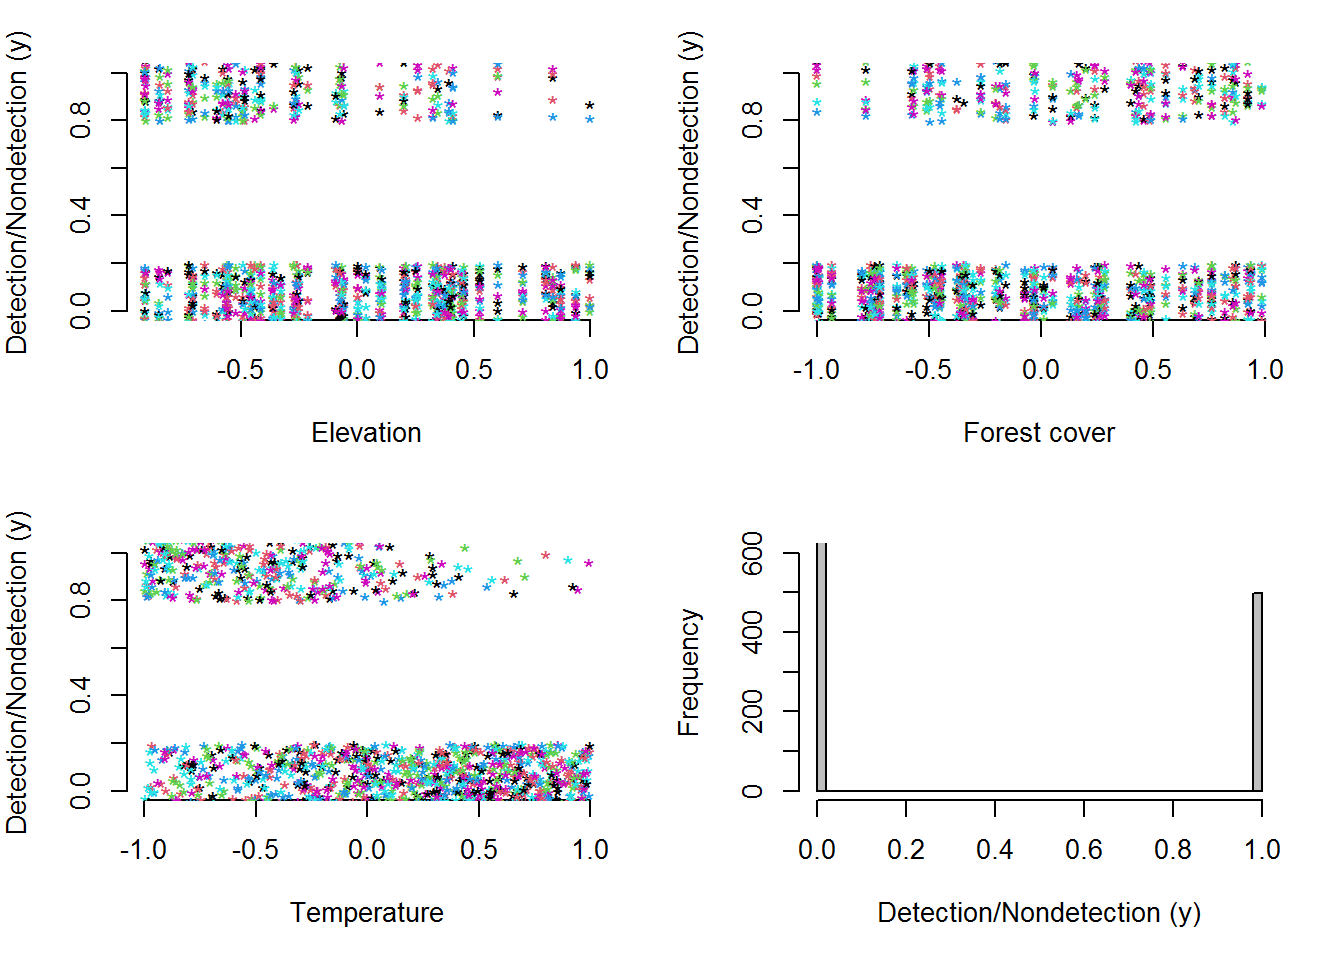
\includegraphics{Occu_Book_files/figure-latex/fig6-1} \caption[fig6]{Relationship between observed (jittered) tapir occupancy (y) and the three standardized covariates. Elevation (A). Forest cover (B). Temperature (C) and the frequency of distribution of the observed occurrence (y) in a data set of 60 sites with 30 samples each (D).}\label{fig:fig6}
\end{figure}

So far we have created a data set where tapir detection/non-detection is negatively correlated with temperature and positively correlated with forest cover. There is a reason why this correlation between variables is different. Occurrence per site, the target of ecological inference, is affected by forest cover and elevation, but not by temperature, while the probability of detection, the parameter characterizing the measurement of the error process when we take occurrence measurements, is also affected by elevation and additionally by temperature. Therefore, as can be seen, there is a great challenge to be able to disentangle the reason for the Spatio-temporal variation in the observation of the detection/non-detection data, given that they can be affected by two totally different processes: the ecological and the observational, that the same covariate can also affect the two processes and that there can also be interactions between those covariates.

\hypertarget{function1}{%
\chapter{Packing everything into a function}\label{function1}}

It could be very useful to pack everything we've done into a single function that allows us to do the same thing many times over and over again. This will allow us to design simulations in a more concise and flexible way and makes the generation of parameters used to generate data more transparent. So let's define a function (which we'll call data.fn) to generate the same data type we just created, assigning arguments to the function, such as sample size, covariate effects, and interaction directions and magnitudes. of the detection error and occupancy terms. This will make our code more flexible and efficient.

\begin{Shaded}
\begin{Highlighting}[]
\DocumentationTok{\#\#\#\#\#\#\#\#\#\#\#\#\#\#\#\#\#\#\#\#\#\#\#\#\#\#\#\#\#\#\#}
\DocumentationTok{\#\# The function starts here }\AlertTok{\#\#\#}
\DocumentationTok{\#\#\#\#\#\#\#\#\#\#\#\#\#\#\#\#\#\#\#\#\#\#\#\#\#\#\#\#\#\#\#}

\CommentTok{\# Function definition with set of default values}
\NormalTok{data.fn }\OtherTok{\textless{}{-}} \ControlFlowTok{function}\NormalTok{(}\AttributeTok{M =} \DecValTok{60}\NormalTok{, }\AttributeTok{J =} \DecValTok{30}\NormalTok{, }\AttributeTok{mean.occupancy =} \FloatTok{0.6}\NormalTok{, }
                    \AttributeTok{beta1 =} \SpecialCharTok{{-}}\DecValTok{2}\NormalTok{, }\AttributeTok{beta2 =} \DecValTok{2}\NormalTok{, }\AttributeTok{beta3 =} \DecValTok{1}\NormalTok{, }\AttributeTok{mean.detection =} \FloatTok{0.3}\NormalTok{, }
                    \AttributeTok{alpha1 =} \SpecialCharTok{{-}}\DecValTok{1}\NormalTok{, }\AttributeTok{alpha2 =} \SpecialCharTok{{-}}\DecValTok{3}\NormalTok{, }\AttributeTok{alpha3 =} \DecValTok{0}\NormalTok{, }\AttributeTok{show.plot =} \ConstantTok{TRUE}\NormalTok{)\{}
\CommentTok{\# Function to simulate occupancy measurements replicated at M sites during J occasions.}
\CommentTok{\# Population closure is assumed for each site.}
\CommentTok{\# Expected occurrence may be affected by elevation (elev), }
\CommentTok{\# forest cover (forest) and their interaction.}
\CommentTok{\# Expected detection probability may be affected by elevation, }
\CommentTok{\# temperature (temp) and their interaction.}
\CommentTok{\# Function arguments:}
\CommentTok{\#     M: Number of spatial replicates (sites)}
\CommentTok{\#     J: Number of temporal replicates (occasions)}
\CommentTok{\#     mean.occupancy: Mean occurrence at value 0 of occurrence covariates}
\CommentTok{\#     beta1: Main effect of elevation on occurrence}
\CommentTok{\#     beta2: Main effect of forest cover on occurrence}
\CommentTok{\#     beta3: Interaction effect on occurrence of elevation and forest cover}
\CommentTok{\#     mean.detection: Mean detection prob. at value 0 of detection covariates}
\CommentTok{\#     alpha1: Main effect of elevation on detection probability}
\CommentTok{\#     alpha2: Main effect of temperature on detection probability}
\CommentTok{\#     alpha3: Interaction effect on detection of elevation and temperature}
\CommentTok{\#     show.plot: if TRUE, plots of the data will be displayed; }
\CommentTok{\#               set to FALSE if you are running simulations.}

\CommentTok{\# Create covariates}
\NormalTok{elev }\OtherTok{\textless{}{-}} \FunctionTok{runif}\NormalTok{(}\AttributeTok{n =}\NormalTok{ M, }\SpecialCharTok{{-}}\DecValTok{1}\NormalTok{, }\DecValTok{1}\NormalTok{)                         }\CommentTok{\# Scaled elevation}
\NormalTok{forest }\OtherTok{\textless{}{-}} \FunctionTok{runif}\NormalTok{(}\AttributeTok{n =}\NormalTok{ M, }\SpecialCharTok{{-}}\DecValTok{1}\NormalTok{, }\DecValTok{1}\NormalTok{)                       }\CommentTok{\# Scaled forest cover}
\NormalTok{temp }\OtherTok{\textless{}{-}} \FunctionTok{array}\NormalTok{(}\FunctionTok{runif}\NormalTok{(}\AttributeTok{n =}\NormalTok{ M}\SpecialCharTok{*}\NormalTok{J, }\SpecialCharTok{{-}}\DecValTok{1}\NormalTok{, }\DecValTok{1}\NormalTok{), }\AttributeTok{dim =} \FunctionTok{c}\NormalTok{(M, J)) }\CommentTok{\# Scaled temperature}

\CommentTok{\# Model for occurrence}
\NormalTok{beta0 }\OtherTok{\textless{}{-}} \FunctionTok{qlogis}\NormalTok{(mean.occupancy)               }\CommentTok{\# Mean occurrence on link scale}
\NormalTok{psi }\OtherTok{\textless{}{-}} \FunctionTok{plogis}\NormalTok{(beta0 }\SpecialCharTok{+}\NormalTok{ beta1}\SpecialCharTok{*}\NormalTok{elev }\SpecialCharTok{+}\NormalTok{ beta2}\SpecialCharTok{*}\NormalTok{forest }\SpecialCharTok{+}\NormalTok{ beta3}\SpecialCharTok{*}\NormalTok{elev}\SpecialCharTok{*}\NormalTok{forest)}
\NormalTok{z }\OtherTok{\textless{}{-}} \FunctionTok{rbinom}\NormalTok{(}\AttributeTok{n =}\NormalTok{ M, }\AttributeTok{size =} \DecValTok{1}\NormalTok{, }\AttributeTok{prob =}\NormalTok{ psi)      }\CommentTok{\# Realised occurrence}

\CommentTok{\# Plots}
\ControlFlowTok{if}\NormalTok{(show.plot)\{}
  \FunctionTok{par}\NormalTok{(}\AttributeTok{mfrow =} \FunctionTok{c}\NormalTok{(}\DecValTok{2}\NormalTok{, }\DecValTok{2}\NormalTok{), }\AttributeTok{cex.main =} \DecValTok{1}\NormalTok{)}
  \FunctionTok{devAskNewPage}\NormalTok{(}\AttributeTok{ask =} \ConstantTok{TRUE}\NormalTok{)}
  \FunctionTok{curve}\NormalTok{(}\FunctionTok{plogis}\NormalTok{(beta0 }\SpecialCharTok{+}\NormalTok{ beta1}\SpecialCharTok{*}\NormalTok{x), }\SpecialCharTok{{-}}\DecValTok{1}\NormalTok{, }\DecValTok{1}\NormalTok{, }\AttributeTok{col =} \StringTok{"red"}\NormalTok{, }\AttributeTok{frame.plot =} \ConstantTok{FALSE}\NormalTok{, }
      \AttributeTok{ylim =} \FunctionTok{c}\NormalTok{(}\DecValTok{0}\NormalTok{, }\DecValTok{1}\NormalTok{), }\AttributeTok{xlab =} \StringTok{"Elevation"}\NormalTok{, }\AttributeTok{ylab =} \StringTok{"psi"}\NormalTok{, }\AttributeTok{lwd =} \DecValTok{2}\NormalTok{)}
  \FunctionTok{plot}\NormalTok{(elev, psi, }\AttributeTok{frame.plot =} \ConstantTok{FALSE}\NormalTok{, }\AttributeTok{ylim =} \FunctionTok{c}\NormalTok{(}\DecValTok{0}\NormalTok{, }\DecValTok{1}\NormalTok{), }\AttributeTok{xlab =} \StringTok{"Elevation"}\NormalTok{, }
     \AttributeTok{ylab =} \StringTok{""}\NormalTok{)}
  \FunctionTok{curve}\NormalTok{(}\FunctionTok{plogis}\NormalTok{(beta0 }\SpecialCharTok{+}\NormalTok{ beta2}\SpecialCharTok{*}\NormalTok{x), }\SpecialCharTok{{-}}\DecValTok{1}\NormalTok{, }\DecValTok{1}\NormalTok{, }\AttributeTok{col =} \StringTok{"red"}\NormalTok{, }\AttributeTok{frame.plot =} \ConstantTok{FALSE}\NormalTok{, }
      \AttributeTok{ylim =} \FunctionTok{c}\NormalTok{(}\DecValTok{0}\NormalTok{, }\DecValTok{1}\NormalTok{), }\AttributeTok{xlab =} \StringTok{"Forest cover"}\NormalTok{, }\AttributeTok{ylab =} \StringTok{"psi"}\NormalTok{, }\AttributeTok{lwd =} \DecValTok{2}\NormalTok{)}
  \FunctionTok{plot}\NormalTok{(forest, psi, }\AttributeTok{frame.plot =} \ConstantTok{FALSE}\NormalTok{, }\AttributeTok{ylim =} \FunctionTok{c}\NormalTok{(}\DecValTok{0}\NormalTok{, }\DecValTok{1}\NormalTok{), }\AttributeTok{xlab =} \StringTok{"Forest cover"}\NormalTok{, }
     \AttributeTok{ylab =} \StringTok{""}\NormalTok{)}
\NormalTok{\}}

\CommentTok{\# Model for observations}
\NormalTok{y }\OtherTok{\textless{}{-}}\NormalTok{ p }\OtherTok{\textless{}{-}} \FunctionTok{matrix}\NormalTok{(}\ConstantTok{NA}\NormalTok{, }\AttributeTok{nrow =}\NormalTok{ M, }\AttributeTok{ncol =}\NormalTok{ J)}\CommentTok{\# Prepare matrix for y and p}
\NormalTok{alpha0 }\OtherTok{\textless{}{-}} \FunctionTok{qlogis}\NormalTok{(mean.detection)        }\CommentTok{\# mean detection on link scale}
\ControlFlowTok{for}\NormalTok{ (j }\ControlFlowTok{in} \DecValTok{1}\SpecialCharTok{:}\NormalTok{J)\{                         }\CommentTok{\# Generate counts by survey}
\NormalTok{   p[,j] }\OtherTok{\textless{}{-}} \FunctionTok{plogis}\NormalTok{(alpha0 }\SpecialCharTok{+}\NormalTok{ alpha1}\SpecialCharTok{*}\NormalTok{elev }\SpecialCharTok{+}\NormalTok{ alpha2}\SpecialCharTok{*}\NormalTok{temp[,j] }\SpecialCharTok{+}\NormalTok{ alpha3}\SpecialCharTok{*}\NormalTok{elev}\SpecialCharTok{*}\NormalTok{temp[,j])}
\NormalTok{   y[,j] }\OtherTok{\textless{}{-}} \FunctionTok{rbinom}\NormalTok{(}\AttributeTok{n =}\NormalTok{ M, }\AttributeTok{size =} \DecValTok{1}\NormalTok{, }\AttributeTok{prob =}\NormalTok{ z }\SpecialCharTok{*}\NormalTok{ p[,j])}
\NormalTok{\}}

\CommentTok{\# True and observed measures of \textquotesingle{}distribution\textquotesingle{}}
\NormalTok{sumZ }\OtherTok{\textless{}{-}} \FunctionTok{sum}\NormalTok{(z)                     }\CommentTok{\# Total occurrence (all sites)}
\NormalTok{sumZ.obs }\OtherTok{\textless{}{-}} \FunctionTok{sum}\NormalTok{(}\FunctionTok{apply}\NormalTok{(y,}\DecValTok{1}\NormalTok{,max))    }\CommentTok{\# Observed number of occ sites}
\NormalTok{psi.fs.true }\OtherTok{\textless{}{-}} \FunctionTok{sum}\NormalTok{(z) }\SpecialCharTok{/}\NormalTok{ M          }\CommentTok{\# True proportion of occ. sites in sample}
\NormalTok{psi.fs.obs }\OtherTok{\textless{}{-}} \FunctionTok{mean}\NormalTok{(}\FunctionTok{apply}\NormalTok{(y,}\DecValTok{1}\NormalTok{,max)) }\CommentTok{\# Observed proportion of occ. sites in sample}

\CommentTok{\# More plots}
\ControlFlowTok{if}\NormalTok{(show.plot)\{}
  \FunctionTok{par}\NormalTok{(}\AttributeTok{mfrow =} \FunctionTok{c}\NormalTok{(}\DecValTok{2}\NormalTok{, }\DecValTok{2}\NormalTok{))}
  \FunctionTok{curve}\NormalTok{(}\FunctionTok{plogis}\NormalTok{(alpha0 }\SpecialCharTok{+}\NormalTok{ alpha1}\SpecialCharTok{*}\NormalTok{x), }\SpecialCharTok{{-}}\DecValTok{1}\NormalTok{, }\DecValTok{1}\NormalTok{, }\AttributeTok{col =} \StringTok{"red"}\NormalTok{, }
      \AttributeTok{main =} \StringTok{"Relationship p{-}elevation }\SpecialCharTok{\textbackslash{}n}\StringTok{at average temperature"}\NormalTok{, }
      \AttributeTok{xlab =} \StringTok{"Scaled elevation"}\NormalTok{, }\AttributeTok{frame.plot =}\NormalTok{ F)}
  \FunctionTok{matplot}\NormalTok{(elev, p, }\AttributeTok{xlab =} \StringTok{"Scaled elevation"}\NormalTok{, }
        \AttributeTok{main =} \StringTok{"Relationship p{-}elevation}\SpecialCharTok{\textbackslash{}n}\StringTok{ at observed temperature"}\NormalTok{, }
        \AttributeTok{pch =} \StringTok{"*"}\NormalTok{, }\AttributeTok{frame.plot =}\NormalTok{ F)}
  \FunctionTok{curve}\NormalTok{(}\FunctionTok{plogis}\NormalTok{(alpha0 }\SpecialCharTok{+}\NormalTok{ alpha2}\SpecialCharTok{*}\NormalTok{x), }\SpecialCharTok{{-}}\DecValTok{1}\NormalTok{, }\DecValTok{1}\NormalTok{, }\AttributeTok{col =} \StringTok{"red"}\NormalTok{, }
      \AttributeTok{main =} \StringTok{"Relationship p{-}temperature }\SpecialCharTok{\textbackslash{}n}\StringTok{ at average elevation"}\NormalTok{, }
      \AttributeTok{xlab =} \StringTok{"Scaled temperature"}\NormalTok{, }\AttributeTok{frame.plot =}\NormalTok{ F)}
  \FunctionTok{matplot}\NormalTok{(temp, p, }\AttributeTok{xlab =} \StringTok{"Scaled temperature"}\NormalTok{, }
        \AttributeTok{main =} \StringTok{"Relationship p{-}temperature }\SpecialCharTok{\textbackslash{}n}\StringTok{at observed elevation"}\NormalTok{, }
        \AttributeTok{pch =} \StringTok{"*"}\NormalTok{, }\AttributeTok{frame.plot =}\NormalTok{ F)}
\NormalTok{\}}

\CommentTok{\# Output}
\FunctionTok{return}\NormalTok{(}\FunctionTok{list}\NormalTok{(}\AttributeTok{M =}\NormalTok{ M, }\AttributeTok{J =}\NormalTok{ J, }\AttributeTok{mean.occupancy =}\NormalTok{ mean.occupancy, }
            \AttributeTok{beta0 =}\NormalTok{ beta0, }\AttributeTok{beta1 =}\NormalTok{ beta1, }\AttributeTok{beta2 =}\NormalTok{ beta2, }\AttributeTok{beta3 =}\NormalTok{ beta3, }
            \AttributeTok{mean.detection =}\NormalTok{ mean.detection, }
            \AttributeTok{alpha0 =}\NormalTok{ alpha0, }\AttributeTok{alpha1 =}\NormalTok{ alpha1, }\AttributeTok{alpha2 =}\NormalTok{ alpha2, }\AttributeTok{alpha3 =}\NormalTok{ alpha3, }
            \AttributeTok{elev =}\NormalTok{ elev, }\AttributeTok{forest =}\NormalTok{ forest, }\AttributeTok{temp =}\NormalTok{ temp, }
            \AttributeTok{psi =}\NormalTok{ psi, }\AttributeTok{z =}\NormalTok{ z, }\AttributeTok{p =}\NormalTok{ p, }\AttributeTok{y =}\NormalTok{ y, }\AttributeTok{sumZ =}\NormalTok{ sumZ, }\AttributeTok{sumZ.obs =}\NormalTok{ sumZ.obs, }
            \AttributeTok{psi.fs.true =}\NormalTok{ psi.fs.true, }\AttributeTok{psi.fs.obs =}\NormalTok{ psi.fs.obs))}
\NormalTok{\}}

\DocumentationTok{\#\#\#\#\#\#\#\#\#\#\#\#\#\#\#\#\#\#\#\#\#\#\#\#\#\#\#\#\#\#\#}
\DocumentationTok{\#\# The function ends  here  }\AlertTok{\#\#\#}
\DocumentationTok{\#\#\#\#\#\#\#\#\#\#\#\#\#\#\#\#\#\#\#\#\#\#\#\#\#\#\#\#\#\#\#}
\end{Highlighting}
\end{Shaded}

Once we have defined the function and executed its code, we can call it repeatedly and output the results to the screen or assign them to an object in R. So that we can use the dataset stored in the object for detailed analysis.

\begin{Shaded}
\begin{Highlighting}[]
\CommentTok{\# Run this part line by line, taking note of the meaning of the }
\CommentTok{\# model in the comment and hitting Enter after each graph.}
\CommentTok{\# Take in to account that if you do not override all the parameters}
\CommentTok{\# with another value, the function will use the default values.}

\FunctionTok{data.fn}\NormalTok{()                  }\CommentTok{\# Execute function with default arguments}
\FunctionTok{data.fn}\NormalTok{(}\AttributeTok{show.plot =} \ConstantTok{FALSE}\NormalTok{) }\CommentTok{\# same, without plots}
\NormalTok{objeto1 }\OtherTok{\textless{}{-}} \FunctionTok{data.fn}\NormalTok{(}\AttributeTok{M =} \DecValTok{30}\NormalTok{, }\AttributeTok{J =} \DecValTok{10}\NormalTok{, }\AttributeTok{mean.occupancy =} \FloatTok{0.5}\NormalTok{, }
                   \AttributeTok{beta1 =} \SpecialCharTok{{-}}\DecValTok{2}\NormalTok{, }\AttributeTok{beta2 =} \DecValTok{2}\NormalTok{, }\AttributeTok{beta3 =} \DecValTok{1}\NormalTok{, }
                   \AttributeTok{mean.detection =} \FloatTok{0.25}\NormalTok{, }\AttributeTok{alpha1 =} \SpecialCharTok{{-}}\DecValTok{1}\NormalTok{,}
                   \AttributeTok{alpha2 =} \SpecialCharTok{{-}}\DecValTok{3}\NormalTok{, }\AttributeTok{alpha3 =} \DecValTok{0}\NormalTok{, }\AttributeTok{show.plot =} \ConstantTok{TRUE}\NormalTok{) }\CommentTok{\# Explicit defaults}
\end{Highlighting}
\end{Shaded}

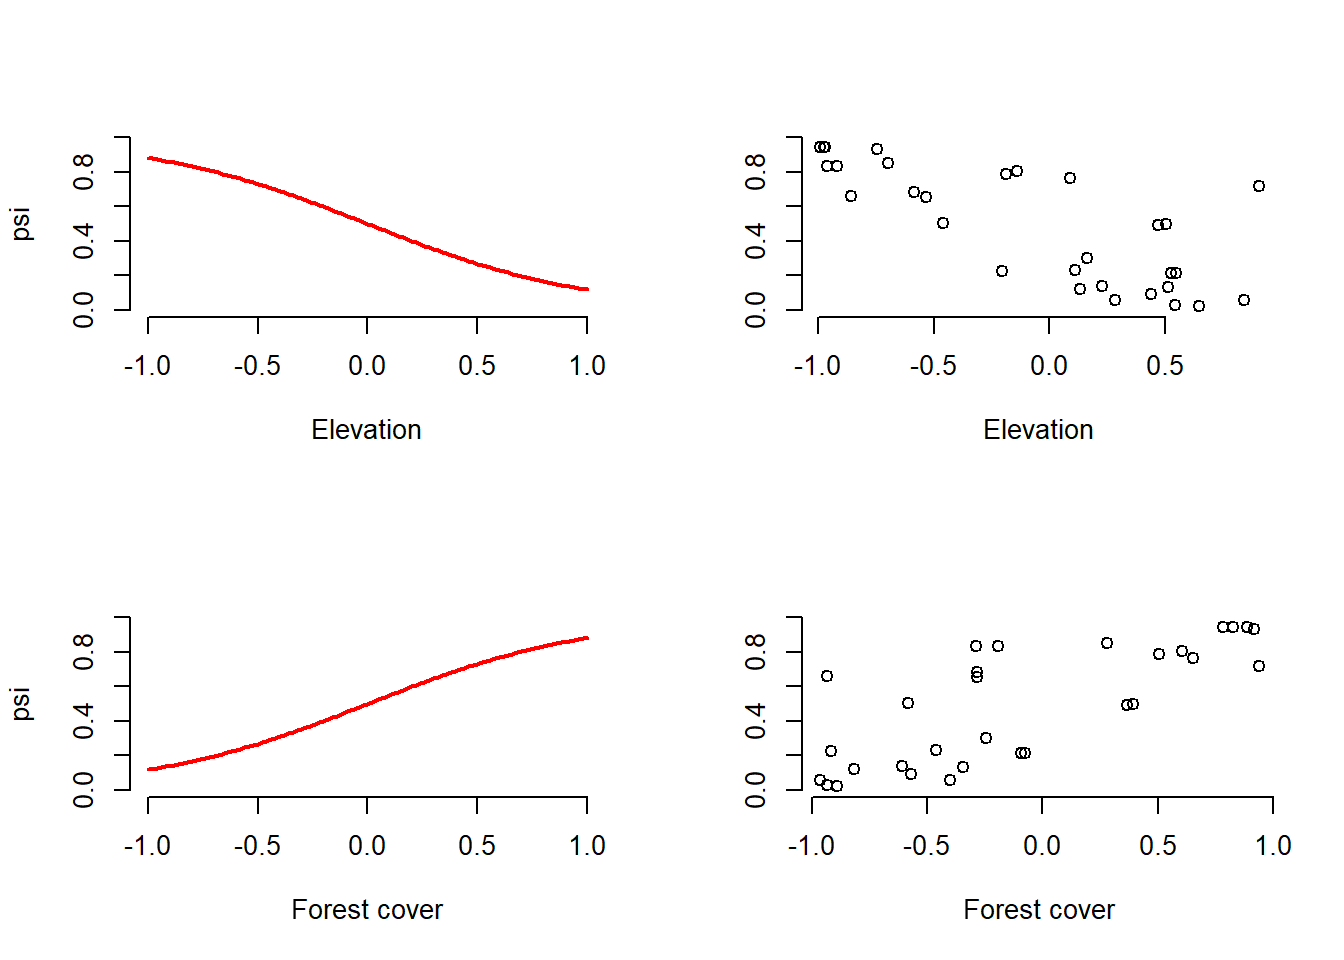
\includegraphics{Occu_Book_files/figure-latex/fun_call1b-1.pdf} 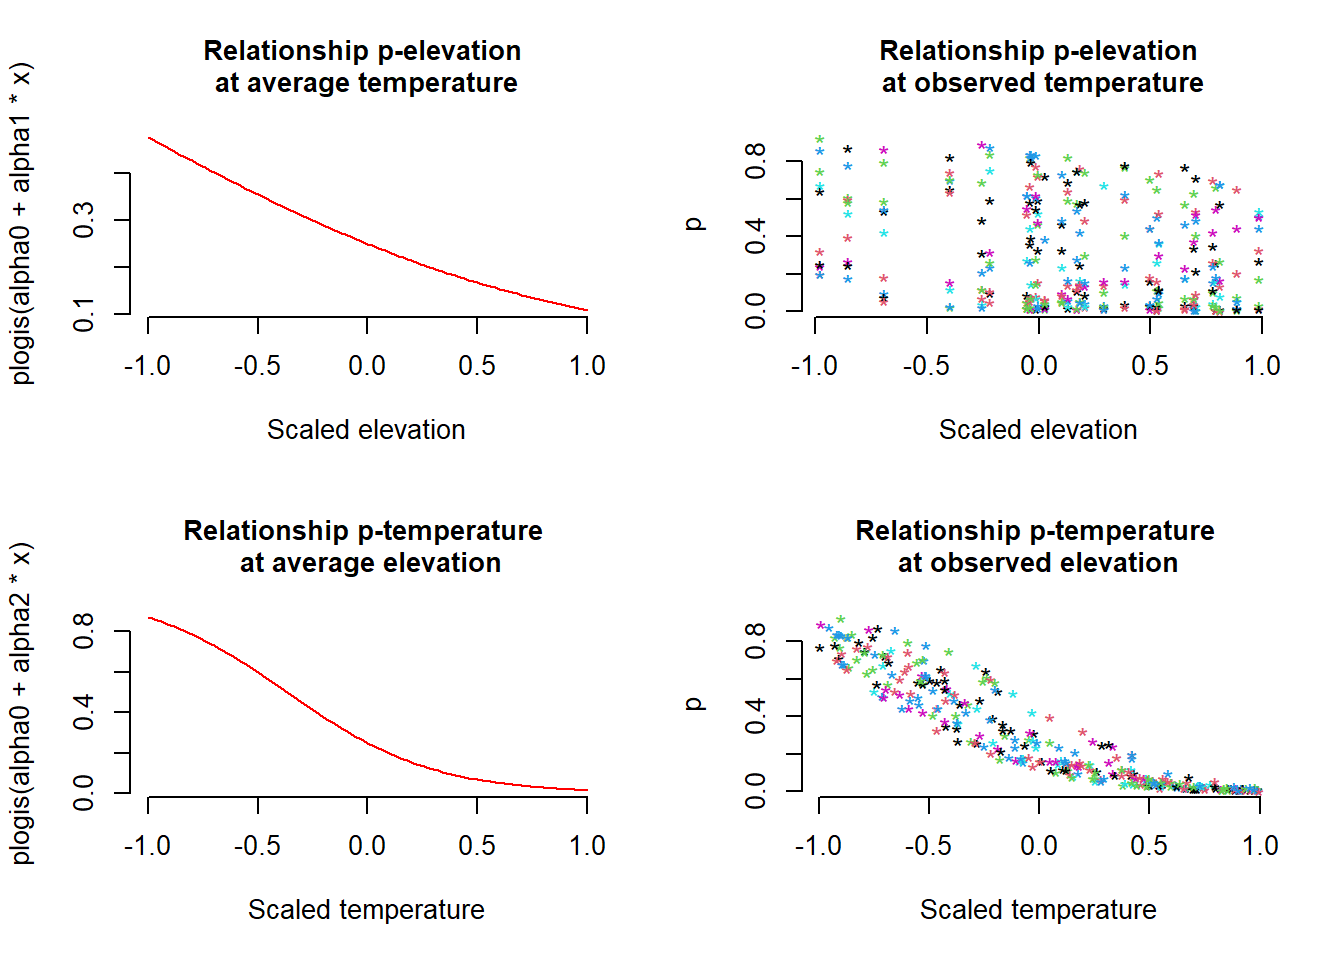
\includegraphics{Occu_Book_files/figure-latex/fun_call1b-2.pdf}

Perhaps the simplest possible use for this function is to experience the sampling error by firsthand: which is the natural variability from repeated runs (several data sets) of our stochastic process by which we compute the data sets. We are going to simulate 10,000 tapir data sets to see how they vary in terms of the true number of occupied sites (sumZ in the code) and the number of sites where tapirs were observed at least once. Note that the data generated in the 10,000 has default parameters in the mean.occupancy and mean.detection parameters.

\begin{Shaded}
\begin{Highlighting}[]
\NormalTok{simrep }\OtherTok{\textless{}{-}} \DecValTok{10000}
\NormalTok{trueSumZ }\OtherTok{\textless{}{-}}\NormalTok{ obsSumZ }\OtherTok{\textless{}{-}} \FunctionTok{numeric}\NormalTok{(simrep)}
\ControlFlowTok{for}\NormalTok{(i }\ControlFlowTok{in} \DecValTok{1}\SpecialCharTok{:}\NormalTok{simrep)\{}
   \ControlFlowTok{if}\NormalTok{(i }\SpecialCharTok{\%\%} \DecValTok{1000} \SpecialCharTok{==}\DecValTok{0}\NormalTok{ )                        }\CommentTok{\# report progress}
   \FunctionTok{cat}\NormalTok{(}\StringTok{"iter"}\NormalTok{, i, }\StringTok{"}\SpecialCharTok{\textbackslash{}n}\StringTok{"}\NormalTok{)}
\NormalTok{   data }\OtherTok{\textless{}{-}} \FunctionTok{data.fn}\NormalTok{(}\AttributeTok{M =} \DecValTok{60}\NormalTok{,}\AttributeTok{J =} \DecValTok{3}\NormalTok{,}\AttributeTok{show.plot =} \ConstantTok{FALSE}\NormalTok{) }\CommentTok{\# 60 sitios, 3 muestreos, p=0.3}
\NormalTok{   trueSumZ[i] }\OtherTok{\textless{}{-}}\NormalTok{ data}\SpecialCharTok{$}\NormalTok{sumZ}
\NormalTok{   obsSumZ[i] }\OtherTok{\textless{}{-}} \FunctionTok{sum}\NormalTok{(}\FunctionTok{apply}\NormalTok{(data}\SpecialCharTok{$}\NormalTok{y, }\DecValTok{1}\NormalTok{, max))}
\NormalTok{\}}
\end{Highlighting}
\end{Shaded}

\begin{verbatim}
## iter 1000 
## iter 2000 
## iter 3000 
## iter 4000 
## iter 5000 
## iter 6000 
## iter 7000 
## iter 8000 
## iter 9000 
## iter 10000
\end{verbatim}

\begin{Shaded}
\begin{Highlighting}[]
\FunctionTok{plot}\NormalTok{(}\FunctionTok{sort}\NormalTok{(trueSumZ), }\AttributeTok{ylim =} \FunctionTok{c}\NormalTok{(}\FunctionTok{min}\NormalTok{(obsSumZ), }\FunctionTok{max}\NormalTok{(trueSumZ)), }\AttributeTok{ylab =} \StringTok{""}\NormalTok{, }\AttributeTok{xlab =} \StringTok{"Simulation"}\NormalTok{,}
     \AttributeTok{col =} \StringTok{"red"}\NormalTok{, }\AttributeTok{main =} \StringTok{"True (red) and observed (blue) number of occupied sites"}\NormalTok{)}
\FunctionTok{points}\NormalTok{(obsSumZ[}\FunctionTok{order}\NormalTok{(trueSumZ)], }\AttributeTok{col =} \StringTok{"blue"}\NormalTok{)}
\end{Highlighting}
\end{Shaded}

\begin{figure}
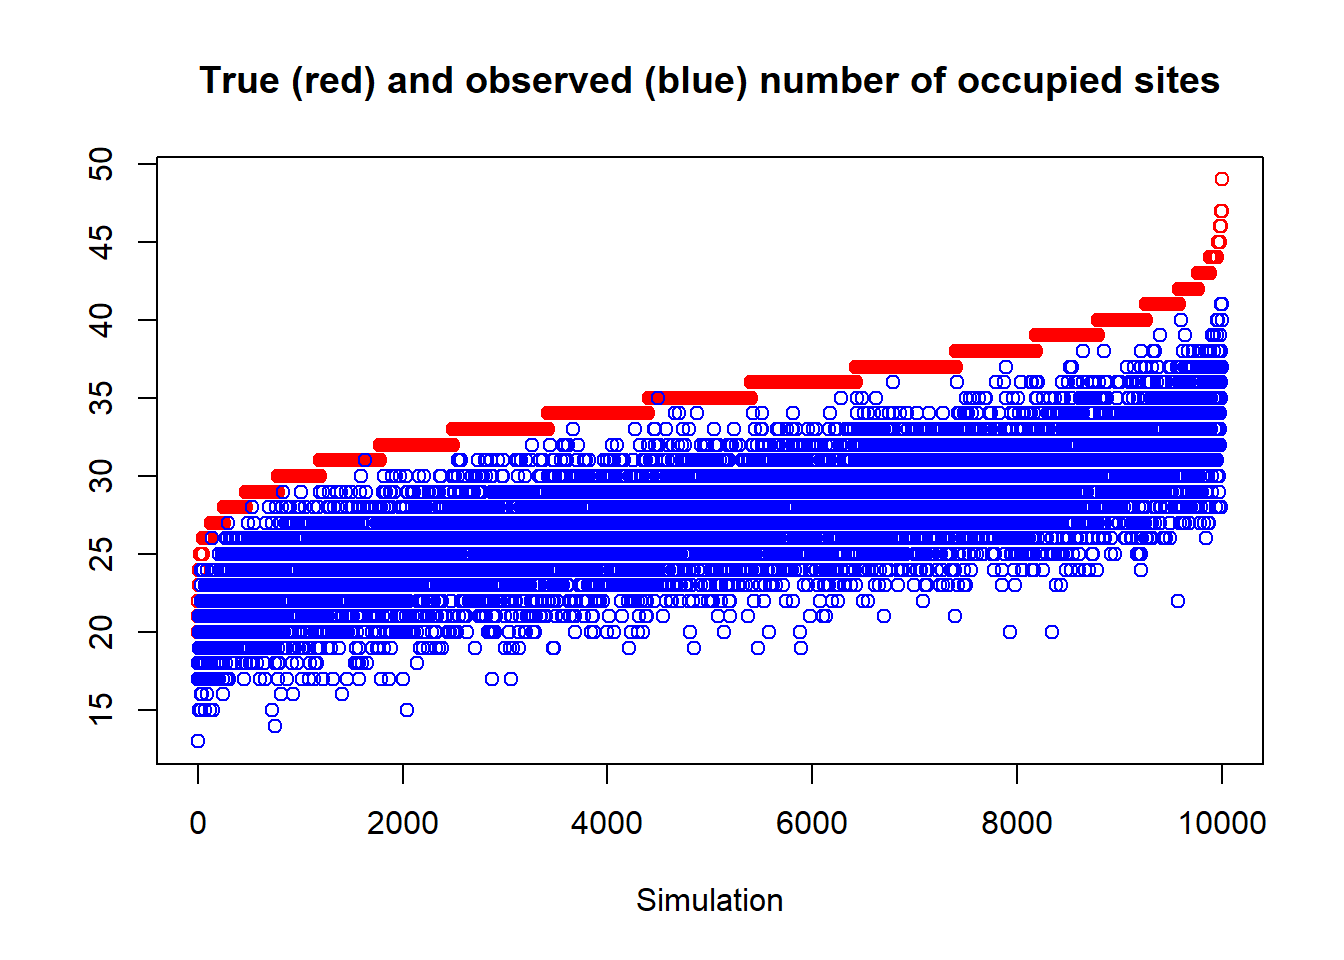
\includegraphics{Occu_Book_files/figure-latex/fig7-1} \caption[fig7]{Natural variability (sampling error) of the true number of occupied sites (ordered by size) in red and the observed number of occupied sites (in blue). The number of sites observed/total is also known as the naïve occupancy of deer occurrence at 60 sites in the simulation. The width of the blue area represents the error induced by imperfect detection. Note the importance of taking this error into account to get a better idea of the occupation.}\label{fig:fig7}
\end{figure}

As an exercise, change the code to again generate the 10,000 simulations with medium (mean.detection =0.5), high (mean.detection =0.8), and perfect detection (mean.detection =1). Compare the resulting graphs.

Now we can use this function to generate data under different sampling schemes, varying the number of sites and the number of repeated samples. As well as under different ecological and detection characteristics, and considering possible interactions between covariates.

\begin{Shaded}
\begin{Highlighting}[]
\CommentTok{\# Run this part line by line, taking note of the meaning of the }
\CommentTok{\# model in the comment and hitting Enter after each graph.}
\CommentTok{\# Take in to account that if you do not override all the parameters}
\CommentTok{\# with another value, the function will use the default values.}

\FunctionTok{data.fn}\NormalTok{(}\AttributeTok{J =} \DecValTok{1}\NormalTok{, }\AttributeTok{show.plot =}\NormalTok{ T)  }\CommentTok{\# Only 1 survey (no temporal replicate)}
\FunctionTok{data.fn}\NormalTok{(}\AttributeTok{J =} \DecValTok{2}\NormalTok{, }\AttributeTok{show.plot =}\NormalTok{ T)  }\CommentTok{\# Only 2 surveys (sites)}
\FunctionTok{data.fn}\NormalTok{(}\AttributeTok{M =} \DecValTok{5}\NormalTok{, }\AttributeTok{J =} \DecValTok{3}\NormalTok{)          }\CommentTok{\# Only 5 sites, 3 counts (repeted visits)}
\FunctionTok{data.fn}\NormalTok{(}\AttributeTok{M =} \DecValTok{1}\NormalTok{, }\AttributeTok{J =} \DecValTok{100}\NormalTok{)        }\CommentTok{\# No spatial replicates, but 100 counts}
\FunctionTok{data.fn}\NormalTok{(}\AttributeTok{M =} \DecValTok{1000}\NormalTok{, }\AttributeTok{J =} \DecValTok{100}\NormalTok{)     }\CommentTok{\# Very intensive sampling. 1000 sites, 100 visits}

\FunctionTok{data.fn}\NormalTok{(}\AttributeTok{mean.occupancy =} \FloatTok{0.6}\NormalTok{,   }\CommentTok{\# psi = 0.6 and}
        \AttributeTok{mean.detection =} \DecValTok{1}\NormalTok{,     }\CommentTok{\# p = 1 (perfect detection!!!)}
        \AttributeTok{show.plot =}\NormalTok{ T)}

\FunctionTok{data.fn}\NormalTok{(}\AttributeTok{mean.occupancy =} \FloatTok{0.95}\NormalTok{,  }\CommentTok{\# psi = 1 a really coomon sp.}
        \AttributeTok{mean.detection =} \DecValTok{1}\NormalTok{,     }\CommentTok{\# p = 1 (perfect detection!!!)}
        \AttributeTok{show.plot =}\NormalTok{ T)}

\FunctionTok{data.fn}\NormalTok{(}\AttributeTok{mean.occupancy =} \FloatTok{0.05}\NormalTok{,  }\CommentTok{\# psi = 0.05 a really rare sp.}
        \AttributeTok{mean.detection =} \FloatTok{0.05}\NormalTok{,  }\CommentTok{\# p = 0.05 and very hard to detect !!!}
        \AttributeTok{show.plot =}\NormalTok{ T)}

\FunctionTok{data.fn}\NormalTok{(}\AttributeTok{beta3 =} \FloatTok{1.5}\NormalTok{, }\AttributeTok{show.plot =} \ConstantTok{TRUE}\NormalTok{) }\CommentTok{\# With interaction elev{-}temp on p}

\FunctionTok{data.fn}\NormalTok{(}\AttributeTok{mean.occupancy =} \FloatTok{0.6}\NormalTok{, }\AttributeTok{beta1 =} \SpecialCharTok{{-}}\DecValTok{2}\NormalTok{, }\AttributeTok{beta2 =} \DecValTok{2}\NormalTok{, }\AttributeTok{beta3 =} \DecValTok{1}\NormalTok{, }
        \AttributeTok{mean.detection =} \FloatTok{0.1}\NormalTok{, }\AttributeTok{show.plot =} \ConstantTok{TRUE}\NormalTok{)  }\CommentTok{\# p = 1 (low detectability)}

\FunctionTok{data.fn}\NormalTok{(}\AttributeTok{M =} \DecValTok{267}\NormalTok{, }\AttributeTok{J =} \DecValTok{5}\NormalTok{, }\AttributeTok{mean.occupancy =} \FloatTok{0.6}\NormalTok{, }\AttributeTok{beta1 =} \DecValTok{0}\NormalTok{, }\AttributeTok{beta2 =} \DecValTok{0}\NormalTok{, }\AttributeTok{beta3 =} \DecValTok{0}\NormalTok{, }
        \AttributeTok{mean.detection =} \FloatTok{0.4}\NormalTok{, }\AttributeTok{alpha1 =} \DecValTok{0}\NormalTok{, }\AttributeTok{alpha2 =} \DecValTok{0}\NormalTok{, }\AttributeTok{alpha3 =} \DecValTok{0}\NormalTok{, }\AttributeTok{show.plot =} \ConstantTok{TRUE}\NormalTok{)}
\CommentTok{\# Simplest case with occupancy (0.6) and detection (0.4) constant, no covariate effects}
\CommentTok{\# observe betas = 0, and alphas = 0. This correspond to a kind of null model.}
\end{Highlighting}
\end{Shaded}

\begin{quote}
\textbf{CONGRATULATIONS!!!, if you got this far, and if you understood the data simulation and its procedure, then you fully understood the basic occupancy model, which is the cornerstone of modern biological sampling and monitoring.}
\end{quote}

\includegraphics{https://media.giphy.com/media/fxsqOYnIMEefC/giphy.gif}

\hypertarget{unmarked}{%
\chapter{Occupancy analysis, ML method}\label{unmarked}}

Now that we have understood how the two processes work and interact; the ecological and the observational to produce the occupation data. After generating several data sets, now we only have to analyze them. The most direct and intuitive way is to use the occu function from the unmarked \citep{Fiske2011} package. Later we can use a Bayesian type model in the BUGS language to analyze the same data and in the end compare which of the two estimators, Maximum Likelihood or Bayesian, is closer to the true parameters.

\hypertarget{clearing-r-memory}{%
\subsection{Clearing R memory}\label{clearing-r-memory}}

Before we continue, and since we have already generated a large amount of data and models in the previous steps, we are going to clear the memory of R before we begin. We do this with the command:

\begin{Shaded}
\begin{Highlighting}[]
\FunctionTok{rm}\NormalTok{(}\AttributeTok{list =} \FunctionTok{ls}\NormalTok{())}
\end{Highlighting}
\end{Shaded}

Once we have done this we must re-run the code of the function that generates the data that we have created in Chapter \ref{function1}.

After having loaded the function again we must return to

\hypertarget{generating-the-data}{%
\section{Generating the data}\label{generating-the-data}}

This time we will use a TEAM-type design (\url{https://www.wildlifeinsights.org/team-network}) with 60 sampling sites and 30 repeated visits, which is equivalent to the 30 days that the cameras remain active in the field. Again our species is the white-tailed tapir. For this example we will assume that detection is 0.6, occupancy is 0.8, and the interactions are much simpler with elevation as the only covariate explaining occupancy. However, for detection there is a more complex relationship, assuming that there is a slight interaction between the observation covariates. For observation, elevation and temperature interact with each other. Also, note how elevation influences in opposite directions with a positive sign at elevation for detection and negative for occupancy.

\begin{Shaded}
\begin{Highlighting}[]
\CommentTok{\# Data generation}
\CommentTok{\# Lets build a model were elevation explain occupancy and p has interactions}
\NormalTok{datos2}\OtherTok{\textless{}{-}}\FunctionTok{data.fn}\NormalTok{(}\AttributeTok{M =} \DecValTok{60}\NormalTok{, }\AttributeTok{J =} \DecValTok{30}\NormalTok{, }\AttributeTok{show.plot =} \ConstantTok{FALSE}\NormalTok{,}
                \AttributeTok{mean.occupancy =} \FloatTok{0.8}\NormalTok{, }\AttributeTok{beta1 =} \SpecialCharTok{{-}}\FloatTok{1.5}\NormalTok{, }\AttributeTok{beta2 =} \DecValTok{0}\NormalTok{, }\AttributeTok{beta3 =} \DecValTok{0}\NormalTok{,  }
                \AttributeTok{mean.detection =} \FloatTok{0.6}\NormalTok{, }\AttributeTok{alpha1 =} \DecValTok{2}\NormalTok{, }\AttributeTok{alpha2 =} \DecValTok{1}\NormalTok{, }\AttributeTok{alpha3 =} \FloatTok{1.5}
\NormalTok{                )}

\CommentTok{\# Function to simulate occupancy measurements replicated at M sites during J occasions.}
\CommentTok{\# Population closure is assumed for each site.}
\CommentTok{\# Expected occurrence may be affected by elevation (elev), }
\CommentTok{\# forest cover (forest) and their interaction.}
\CommentTok{\# Expected detection probability may be affected by elevation, }
\CommentTok{\# temperature (temp) and their interaction.}
\CommentTok{\# Function arguments:}
\CommentTok{\#     M: Number of spatial replicates (sites)}
\CommentTok{\#     J: Number of temporal replicates (occasions)}
\CommentTok{\#     mean.occupancy: Mean occurrence at value 0 of occurrence covariates}
\CommentTok{\#     beta1: Main effect of elevation on occurrence}
\CommentTok{\#     beta2: Main effect of forest cover on occurrence}
\CommentTok{\#     beta3: Interaction effect on occurrence of elevation and forest cover}
\CommentTok{\#     mean.detection: Mean detection prob. at value 0 of detection covariates}
\CommentTok{\#     alpha1: Main effect of elevation on detection probability}
\CommentTok{\#     alpha2: Main effect of temperature on detection probability}
\CommentTok{\#     alpha3: Interaction effect on detection of elevation and temperature}
\CommentTok{\#     show.plot: if TRUE, plots of the data will be displayed; }
\CommentTok{\#               set to FALSE if you are running simulations.}


\CommentTok{\#To make the objects inside the list directly accessible to R, without having to address }
\CommentTok{\#them as data$C for instance, you can attach datos2 to the search path.}

\FunctionTok{attach}\NormalTok{(datos2)         }\CommentTok{\# Make objects inside of \textquotesingle{}datos2\textquotesingle{} accessible directly}

\CommentTok{\#Remember to detach the data after use, and in particular before attaching a new data }
\CommentTok{\#object, because more than one data set attached in the search path will cause confusion.}

\CommentTok{\# detach(datos2)         \# Make clean up}
\end{Highlighting}
\end{Shaded}

\hypertarget{putting-the-data-in-unmarked}{%
\section{Putting the data in unmarked}\label{putting-the-data-in-unmarked}}

\href{http://cran.r-project.org/web/packages/unmarked/index.html}{Unmarked} is the R package we use to analyze the \citep{Fiske2011} occupancy data. To achieve this we must first prepare the data and collect it in an object of type unmarkedFrame. In this case we use the unmarkedFrameOccu function, which is specific for occupancy analysis of a single season or season. More about unmarked at: \url{https://sites.google.com/site/unmarkedinfo/home}

\begin{Shaded}
\begin{Highlighting}[]
\FunctionTok{library}\NormalTok{(unmarked)}
\NormalTok{siteCovs }\OtherTok{\textless{}{-}} \FunctionTok{as.data.frame}\NormalTok{(}\FunctionTok{cbind}\NormalTok{(forest,elev)) }\CommentTok{\# occupancy covariates }
\NormalTok{obselev}\OtherTok{\textless{}{-}}\FunctionTok{matrix}\NormalTok{(}\FunctionTok{rep}\NormalTok{(elev,J),}\AttributeTok{ncol =}\NormalTok{ J) }\CommentTok{\# make elevation per observation}
\NormalTok{obsCovs }\OtherTok{\textless{}{-}} \FunctionTok{list}\NormalTok{(}\AttributeTok{temp=}\NormalTok{ temp,}\AttributeTok{elev=}\NormalTok{obselev) }\CommentTok{\# detection covariates}

\CommentTok{\# umf is the object joining observations (y), occupancy covariates (siteCovs)}
\CommentTok{\# and detection covariates (obsCovs). Note that obsCovs should be a list of }
\CommentTok{\# matrices or dataframes.}

\NormalTok{umf }\OtherTok{\textless{}{-}} \FunctionTok{unmarkedFrameOccu}\NormalTok{(}\AttributeTok{y =}\NormalTok{ y, }\AttributeTok{siteCovs =}\NormalTok{ siteCovs, }\AttributeTok{obsCovs =}\NormalTok{ obsCovs)}
\end{Highlighting}
\end{Shaded}

The unmarked package allows us to graphically see how the data is arranged at the sampling sites with the plot function.

\begin{Shaded}
\begin{Highlighting}[]
\FunctionTok{plot}\NormalTok{ (umf)}
\end{Highlighting}
\end{Shaded}

\begin{figure}
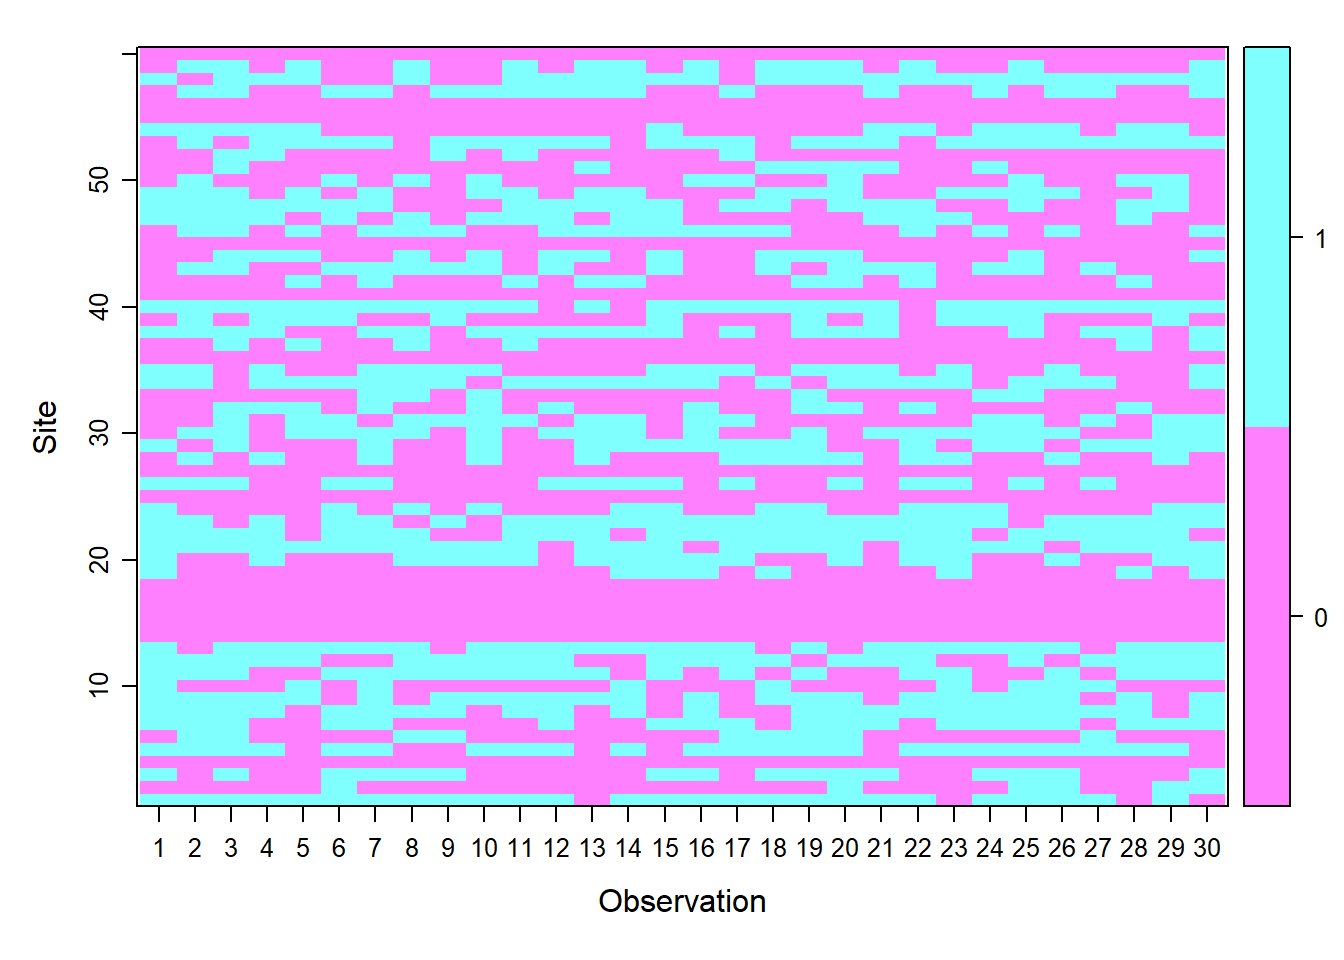
\includegraphics{Occu_Book_files/figure-latex/umfplot-1} \caption[fig]{Inspección grafica del objeto umf.}\label{fig:umfplot}
\end{figure}

\hypertarget{fitting-the-models}{%
\section{Fitting the models}\label{fitting-the-models}}

The next step is to fit the models that were required by varying the covariates. This is accomplished with the \href{http://www.rdocumentation.org/packages/unmarked/versions/0.11-0/topics/occu}{occu() function}.

Keep in mind that in the model building process your models must have a biological meaning.

\begin{Shaded}
\begin{Highlighting}[]
\CommentTok{\# detection first, occupancy next}
\NormalTok{fm0 }\OtherTok{\textless{}{-}} \FunctionTok{occu}\NormalTok{(}\SpecialCharTok{\textasciitilde{}}\DecValTok{1} \SpecialCharTok{\textasciitilde{}}\DecValTok{1}\NormalTok{, umf) }\CommentTok{\# Null model}
\NormalTok{fm1 }\OtherTok{\textless{}{-}} \FunctionTok{occu}\NormalTok{(}\SpecialCharTok{\textasciitilde{}}\NormalTok{ elev }\SpecialCharTok{\textasciitilde{}} \DecValTok{1}\NormalTok{, umf) }\CommentTok{\# elev explaining detection}
\NormalTok{fm2 }\OtherTok{\textless{}{-}} \FunctionTok{occu}\NormalTok{(}\SpecialCharTok{\textasciitilde{}}\NormalTok{ elev }\SpecialCharTok{\textasciitilde{}}\NormalTok{ elev, umf) }\CommentTok{\# elev explaining detection and occupancy}
\NormalTok{fm3 }\OtherTok{\textless{}{-}} \FunctionTok{occu}\NormalTok{(}\SpecialCharTok{\textasciitilde{}}\NormalTok{ temp }\SpecialCharTok{\textasciitilde{}}\NormalTok{ elev, umf)}
\NormalTok{fm4 }\OtherTok{\textless{}{-}} \FunctionTok{occu}\NormalTok{(}\SpecialCharTok{\textasciitilde{}}\NormalTok{ temp }\SpecialCharTok{\textasciitilde{}}\NormalTok{ forest, umf)}
\NormalTok{fm5 }\OtherTok{\textless{}{-}} \FunctionTok{occu}\NormalTok{(}\SpecialCharTok{\textasciitilde{}}\NormalTok{ elev }\SpecialCharTok{+}\NormalTok{ temp }\SpecialCharTok{\textasciitilde{}} \DecValTok{1}\NormalTok{, umf)}
\NormalTok{fm6 }\OtherTok{\textless{}{-}} \FunctionTok{occu}\NormalTok{(}\SpecialCharTok{\textasciitilde{}}\NormalTok{ elev }\SpecialCharTok{+}\NormalTok{ temp }\SpecialCharTok{+}\NormalTok{ elev}\SpecialCharTok{:}\NormalTok{temp }\SpecialCharTok{\textasciitilde{}} \DecValTok{1}\NormalTok{, umf)}
\NormalTok{fm7 }\OtherTok{\textless{}{-}} \FunctionTok{occu}\NormalTok{(}\SpecialCharTok{\textasciitilde{}}\NormalTok{ elev }\SpecialCharTok{+}\NormalTok{ temp }\SpecialCharTok{+}\NormalTok{ elev}\SpecialCharTok{:}\NormalTok{temp }\SpecialCharTok{\textasciitilde{}}\NormalTok{ elev, umf)}
\NormalTok{fm8 }\OtherTok{\textless{}{-}} \FunctionTok{occu}\NormalTok{(}\SpecialCharTok{\textasciitilde{}}\NormalTok{ elev }\SpecialCharTok{+}\NormalTok{ temp }\SpecialCharTok{+}\NormalTok{ elev}\SpecialCharTok{:}\NormalTok{temp }\SpecialCharTok{\textasciitilde{}}\NormalTok{ forest, umf)}
\end{Highlighting}
\end{Shaded}

\hypertarget{model-selection}{%
\section{Model Selection}\label{model-selection}}

Unmarked allows you to perform a model selection procedure to select models based on the Akaike information Criterium (AIC) of each one. So the lowest AIC is the most parsimonious model according to our data \citep{Burnham2004}.

\begin{Shaded}
\begin{Highlighting}[]
\NormalTok{models }\OtherTok{\textless{}{-}} \FunctionTok{fitList}\NormalTok{( }\CommentTok{\# here e put names to the models}
  \StringTok{\textquotesingle{}p(.)psi(.)\textquotesingle{}}                        \OtherTok{=}\NormalTok{ fm0,}
  \StringTok{\textquotesingle{}p(elev)psi(.)\textquotesingle{}}                     \OtherTok{=}\NormalTok{ fm1,}
  \StringTok{\textquotesingle{}p(elev)psi(elev)\textquotesingle{}}                  \OtherTok{=}\NormalTok{ fm2,}
  \StringTok{\textquotesingle{}p(temp)psi(elev)\textquotesingle{}}                  \OtherTok{=}\NormalTok{ fm3,}
  \StringTok{\textquotesingle{}p(temp)psi(forest)\textquotesingle{}}                \OtherTok{=}\NormalTok{ fm4,}
  \StringTok{\textquotesingle{}p(temp+elev)psi(.)\textquotesingle{}}                \OtherTok{=}\NormalTok{ fm5,}
  \StringTok{\textquotesingle{}p(temp+elev+elev:temp)psi(.)\textquotesingle{}}      \OtherTok{=}\NormalTok{ fm6,}
  \StringTok{\textquotesingle{}p(temp+elev+elev:temp)psi(elev)\textquotesingle{}}   \OtherTok{=}\NormalTok{ fm7,}
  \StringTok{\textquotesingle{}p(temp+elev+elev:temp)psi(forest)\textquotesingle{}} \OtherTok{=}\NormalTok{ fm8)}

\FunctionTok{modSel}\NormalTok{(models) }\CommentTok{\# model selection procedure}
\end{Highlighting}
\end{Shaded}

\begin{verbatim}
##                                   nPars
## p(temp+elev+elev:temp)psi(elev)       6
## p(temp+elev+elev:temp)psi(.)          5
## p(temp+elev+elev:temp)psi(forest)     6
## p(temp+elev)psi(.)                    4
## p(elev)psi(elev)                      4
## p(elev)psi(.)                         3
## p(temp)psi(elev)                      4
## p(temp)psi(forest)                    4
## p(.)psi(.)                            2
##                                       AIC
## p(temp+elev+elev:temp)psi(elev)   1630.77
## p(temp+elev+elev:temp)psi(.)      1636.27
## p(temp+elev+elev:temp)psi(forest) 1638.24
## p(temp+elev)psi(.)                1672.55
## p(elev)psi(elev)                  1741.34
## p(elev)psi(.)                     1746.83
## p(temp)psi(elev)                  1898.56
## p(temp)psi(forest)                1906.03
## p(.)psi(.)                        1969.25
##                                    delta
## p(temp+elev+elev:temp)psi(elev)     0.00
## p(temp+elev+elev:temp)psi(.)        5.49
## p(temp+elev+elev:temp)psi(forest)   7.47
## p(temp+elev)psi(.)                 41.78
## p(elev)psi(elev)                  110.57
## p(elev)psi(.)                     116.06
## p(temp)psi(elev)                  267.79
## p(temp)psi(forest)                275.26
## p(.)psi(.)                        338.48
##                                     AICwt
## p(temp+elev+elev:temp)psi(elev)   9.2e-01
## p(temp+elev+elev:temp)psi(.)      5.9e-02
## p(temp+elev+elev:temp)psi(forest) 2.2e-02
## p(temp+elev)psi(.)                7.8e-10
## p(elev)psi(elev)                  9.0e-25
## p(elev)psi(.)                     5.8e-26
## p(temp)psi(elev)                  6.5e-59
## p(temp)psi(forest)                1.6e-60
## p(.)psi(.)                        2.9e-74
##                                   cumltvWt
## p(temp+elev+elev:temp)psi(elev)       0.92
## p(temp+elev+elev:temp)psi(.)          0.98
## p(temp+elev+elev:temp)psi(forest)     1.00
## p(temp+elev)psi(.)                    1.00
## p(elev)psi(elev)                      1.00
## p(elev)psi(.)                         1.00
## p(temp)psi(elev)                      1.00
## p(temp)psi(forest)                    1.00
## p(.)psi(.)                            1.00
\end{verbatim}

\hypertarget{prediction-in-graphs}{%
\section{Prediction in graphs}\label{prediction-in-graphs}}

The model with the lowest AIC can be used to predict expected results according to a new data set. For example, one might ask the expected abundance of deer at a higher elevation site. Predictions are also another way of presenting the results of an analysis. Here we will illustrate what the prediction of \(\psi\) and \emph{p} looks like over the range of covariates studied. Note that we are using standardized covariates. If we were using covariates at their real scale, we would have to take into account that they have to be transformed using the mean and standard deviation.

Before using the model to predict it is a good idea to check the model parameters and their errors, then check graphically that the model fits well with the parboot function, which does a resampling of the model. This plot is interpreted as the model having a good fit, when the mean (dotted line) is between the intervals of the histogram. If the line is too far from the histogram the model might not be good at predicting.

\begin{Shaded}
\begin{Highlighting}[]
\FunctionTok{summary}\NormalTok{(fm7) }\CommentTok{\# see the model parameters}
\end{Highlighting}
\end{Shaded}

\begin{verbatim}
## 
## Call:
## occu(formula = ~elev + temp + elev:temp ~ elev, data = umf)
## 
## Occupancy (logit-scale):
##             Estimate    SE     z  P(>|z|)
## (Intercept)     1.41 0.366  3.85 0.000117
## elev           -1.63 0.656 -2.48 0.013082
## 
## Detection (logit-scale):
##             Estimate     SE     z
## (Intercept)     0.53 0.0698  7.60
## elev            1.80 0.1277 14.10
## temp            1.16 0.1209  9.57
## elev:temp       1.33 0.2211  6.00
##              P(>|z|)
## (Intercept) 3.04e-14
## elev        3.56e-45
## temp        1.08e-21
## elev:temp   1.96e-09
## 
## AIC: 1630.771 
## Number of sites: 60
## optim convergence code: 0
## optim iterations: 31 
## Bootstrap iterations: 0
\end{verbatim}

\begin{Shaded}
\begin{Highlighting}[]
\NormalTok{pb }\OtherTok{\textless{}{-}} \FunctionTok{parboot}\NormalTok{(fm7, }\AttributeTok{nsim=}\DecValTok{250}\NormalTok{, }\AttributeTok{report=}\DecValTok{10}\NormalTok{) }\CommentTok{\# goodness of fit}
\end{Highlighting}
\end{Shaded}

\begin{verbatim}
## t0 = 409.3793
\end{verbatim}

\begin{Shaded}
\begin{Highlighting}[]
\FunctionTok{plot}\NormalTok{ (pb) }\CommentTok{\# plot goodness of fit}
\end{Highlighting}
\end{Shaded}

\begin{figure}
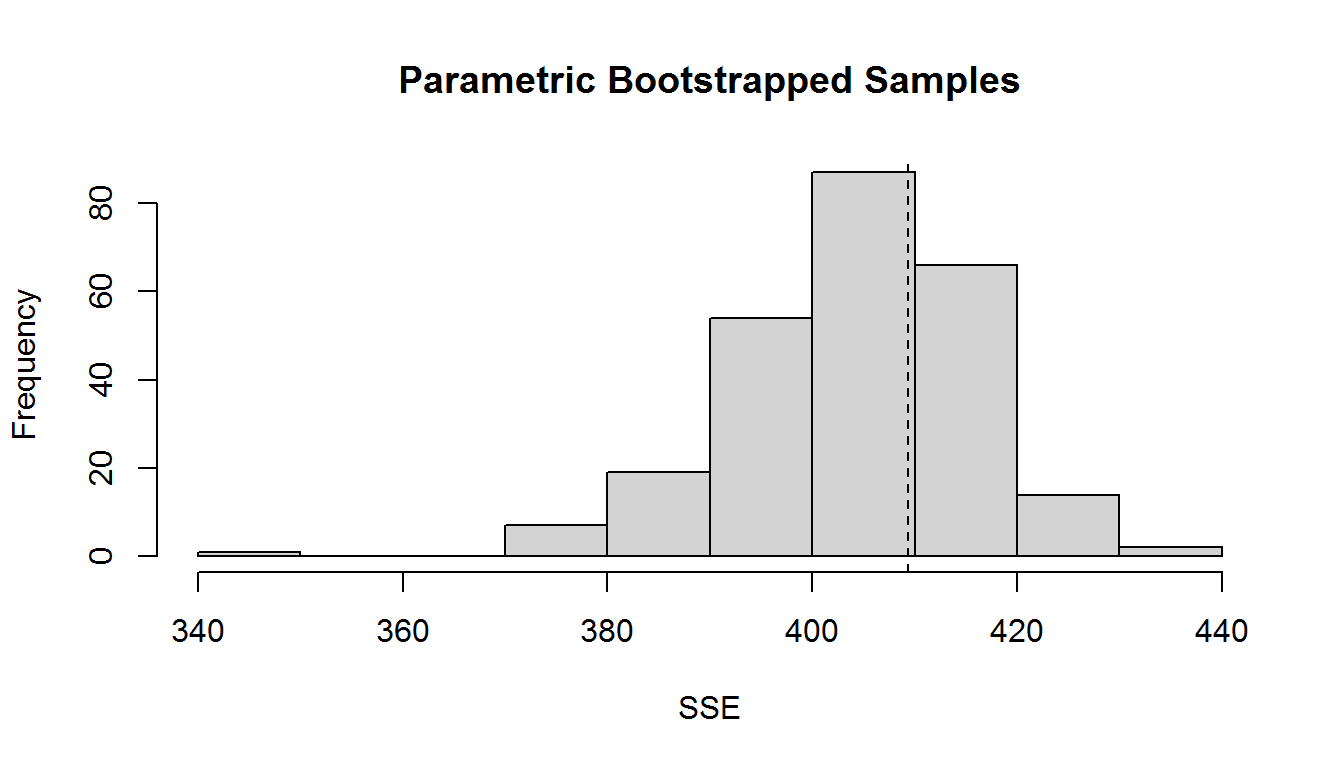
\includegraphics{Occu_Book_files/figure-latex/fit1-1} \caption[fig]{Graphical evaluation of the model fit fm7.}\label{fig:fit1}
\end{figure}

Now that we know that our best model has a good fit, we can use it to predict occupancy in the altitude range to see how it behaves on a graph.

\begin{Shaded}
\begin{Highlighting}[]
\NormalTok{elevrange}\OtherTok{\textless{}{-}}\FunctionTok{data.frame}\NormalTok{(}\AttributeTok{elev=}\FunctionTok{seq}\NormalTok{(}\FunctionTok{min}\NormalTok{(datos2}\SpecialCharTok{$}\NormalTok{elev),}\FunctionTok{max}\NormalTok{(datos2}\SpecialCharTok{$}\NormalTok{elev),}\AttributeTok{length=}\DecValTok{100}\NormalTok{)) }\CommentTok{\# newdata}
\NormalTok{pred\_psi }\OtherTok{\textless{}{-}}\FunctionTok{predict}\NormalTok{(fm7,}\AttributeTok{type=}\StringTok{"state"}\NormalTok{,}\AttributeTok{newdata=}\NormalTok{elevrange,}\AttributeTok{appendData=}\ConstantTok{TRUE}\NormalTok{) }
\FunctionTok{plot}\NormalTok{(Predicted}\SpecialCharTok{\textasciitilde{}}\NormalTok{elev, pred\_psi,}\AttributeTok{type=}\StringTok{"l"}\NormalTok{,}\AttributeTok{col=}\StringTok{"blue"}\NormalTok{,}
       \AttributeTok{xlab=}\StringTok{"elev"}\NormalTok{,}
       \AttributeTok{ylab=}\StringTok{"psi"}\NormalTok{)}
\FunctionTok{lines}\NormalTok{(lower}\SpecialCharTok{\textasciitilde{}}\NormalTok{elev, pred\_psi,}\AttributeTok{type=}\StringTok{"l"}\NormalTok{,}\AttributeTok{col=}\FunctionTok{gray}\NormalTok{(}\FloatTok{0.5}\NormalTok{))}
\FunctionTok{lines}\NormalTok{(upper}\SpecialCharTok{\textasciitilde{}}\NormalTok{elev, pred\_psi,}\AttributeTok{type=}\StringTok{"l"}\NormalTok{,}\AttributeTok{col=}\FunctionTok{gray}\NormalTok{(}\FloatTok{0.5}\NormalTok{))}
\end{Highlighting}
\end{Shaded}

\begin{figure}
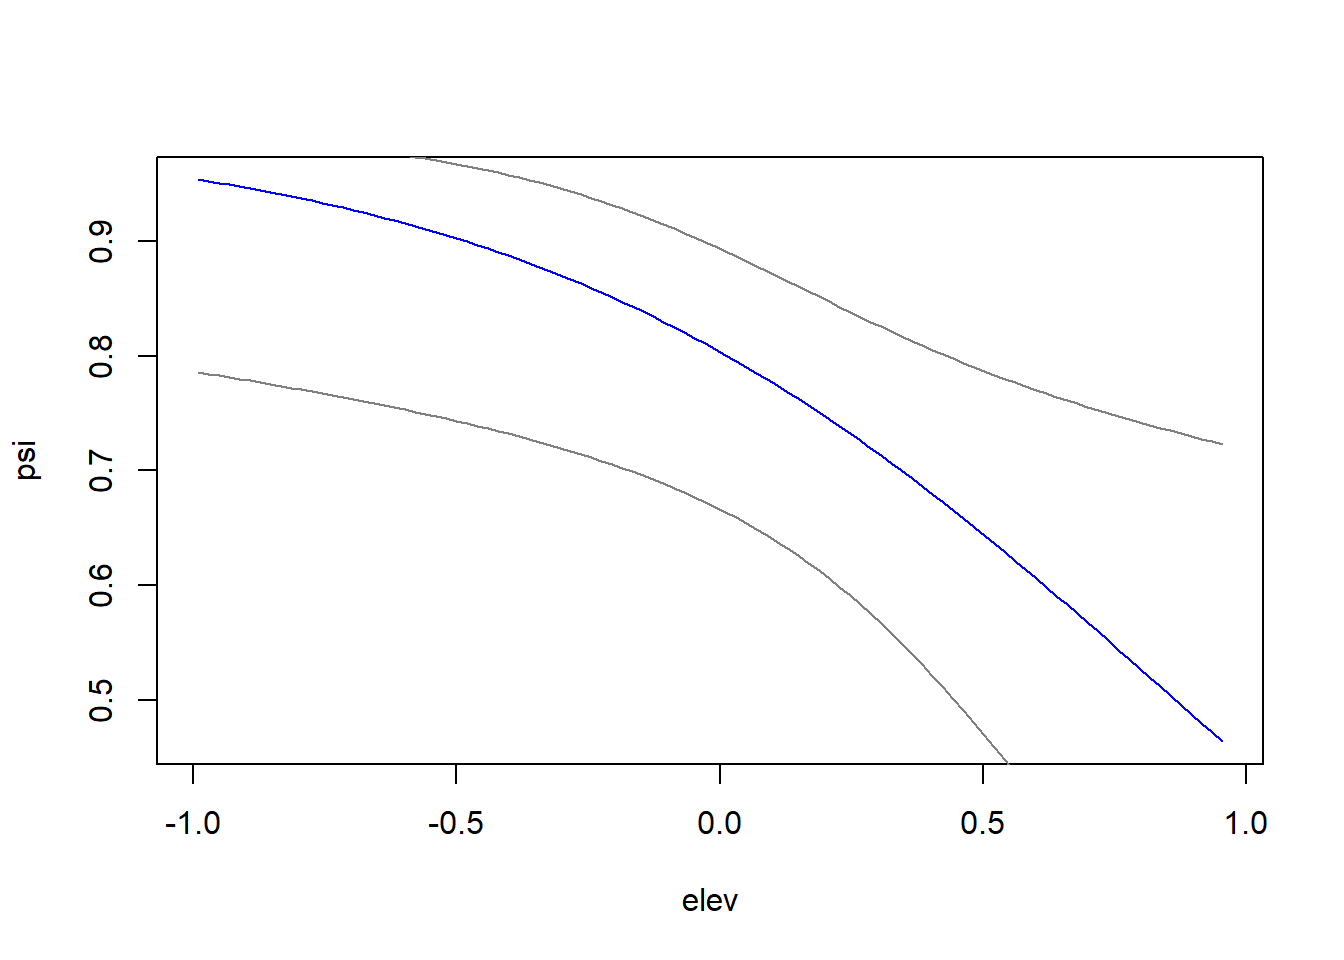
\includegraphics{Occu_Book_files/figure-latex/gpsi-1} \caption[fig.]{Plot of occupancy versus elevation.}\label{fig:gpsi}
\end{figure}

\hypertarget{spatially-explicit-prediction}{%
\section{Spatially explicit prediction}\label{spatially-explicit-prediction}}

We can also use the best model to predict spatially explicitly if we have the maps. As an illustration we will construct simulated maps for each of our covariates. The maps arise from a random pattern of points with a Poisson distribution. We then convert these points to an interpolated surface.

\begin{Shaded}
\begin{Highlighting}[]
\CommentTok{\# lets make random maps for the three covariates}
\FunctionTok{library}\NormalTok{(raster)}
\FunctionTok{library}\NormalTok{(spatstat)}
\FunctionTok{set.seed}\NormalTok{(}\DecValTok{24}\NormalTok{) }\CommentTok{\# Remove for random simulations}

\CommentTok{\# CONSTRUCT ANALYSIS WINDOW USING THE FOLLOWING:}
\NormalTok{xrange}\OtherTok{=}\FunctionTok{c}\NormalTok{(}\SpecialCharTok{{-}}\FloatTok{2.5}\NormalTok{, }\FloatTok{1002.5}\NormalTok{)}
\NormalTok{yrange}\OtherTok{=}\FunctionTok{c}\NormalTok{(}\SpecialCharTok{{-}}\FloatTok{2.5}\NormalTok{, }\FloatTok{502.5}\NormalTok{)}
\NormalTok{window}\OtherTok{\textless{}{-}}\FunctionTok{owin}\NormalTok{(xrange, yrange)}

\CommentTok{\# Build maps from random points and interpole in same line}
\NormalTok{elev   }\OtherTok{\textless{}{-}} \FunctionTok{density}\NormalTok{(}\FunctionTok{rpoispp}\NormalTok{(}\AttributeTok{lambda=}\FloatTok{0.6}\NormalTok{, }\AttributeTok{win=}\NormalTok{window)) }\CommentTok{\# }
\NormalTok{forest }\OtherTok{\textless{}{-}} \FunctionTok{density}\NormalTok{(}\FunctionTok{rpoispp}\NormalTok{(}\AttributeTok{lambda=}\FloatTok{0.2}\NormalTok{, }\AttributeTok{win=}\NormalTok{window)) }\CommentTok{\# }
\NormalTok{temp   }\OtherTok{\textless{}{-}} \FunctionTok{density}\NormalTok{(}\FunctionTok{rpoispp}\NormalTok{(}\AttributeTok{lambda=}\FloatTok{0.5}\NormalTok{, }\AttributeTok{win=}\NormalTok{window)) }\CommentTok{\# }

\CommentTok{\# Convert covs to raster and Put in the same stack }
\NormalTok{mapdata.m}\OtherTok{\textless{}{-}}\FunctionTok{stack}\NormalTok{(}\FunctionTok{raster}\NormalTok{(elev),}\FunctionTok{raster}\NormalTok{(forest), }\FunctionTok{raster}\NormalTok{(temp)) }
\FunctionTok{names}\NormalTok{(mapdata.m)}\OtherTok{\textless{}{-}} \FunctionTok{c}\NormalTok{(}\StringTok{"elev"}\NormalTok{, }\StringTok{"forest"}\NormalTok{, }\StringTok{"temp"}\NormalTok{) }\CommentTok{\# put names to raster}

\CommentTok{\# lets plot the covs maps}
\FunctionTok{plot}\NormalTok{(mapdata.m)}
\end{Highlighting}
\end{Shaded}

\begin{figure}
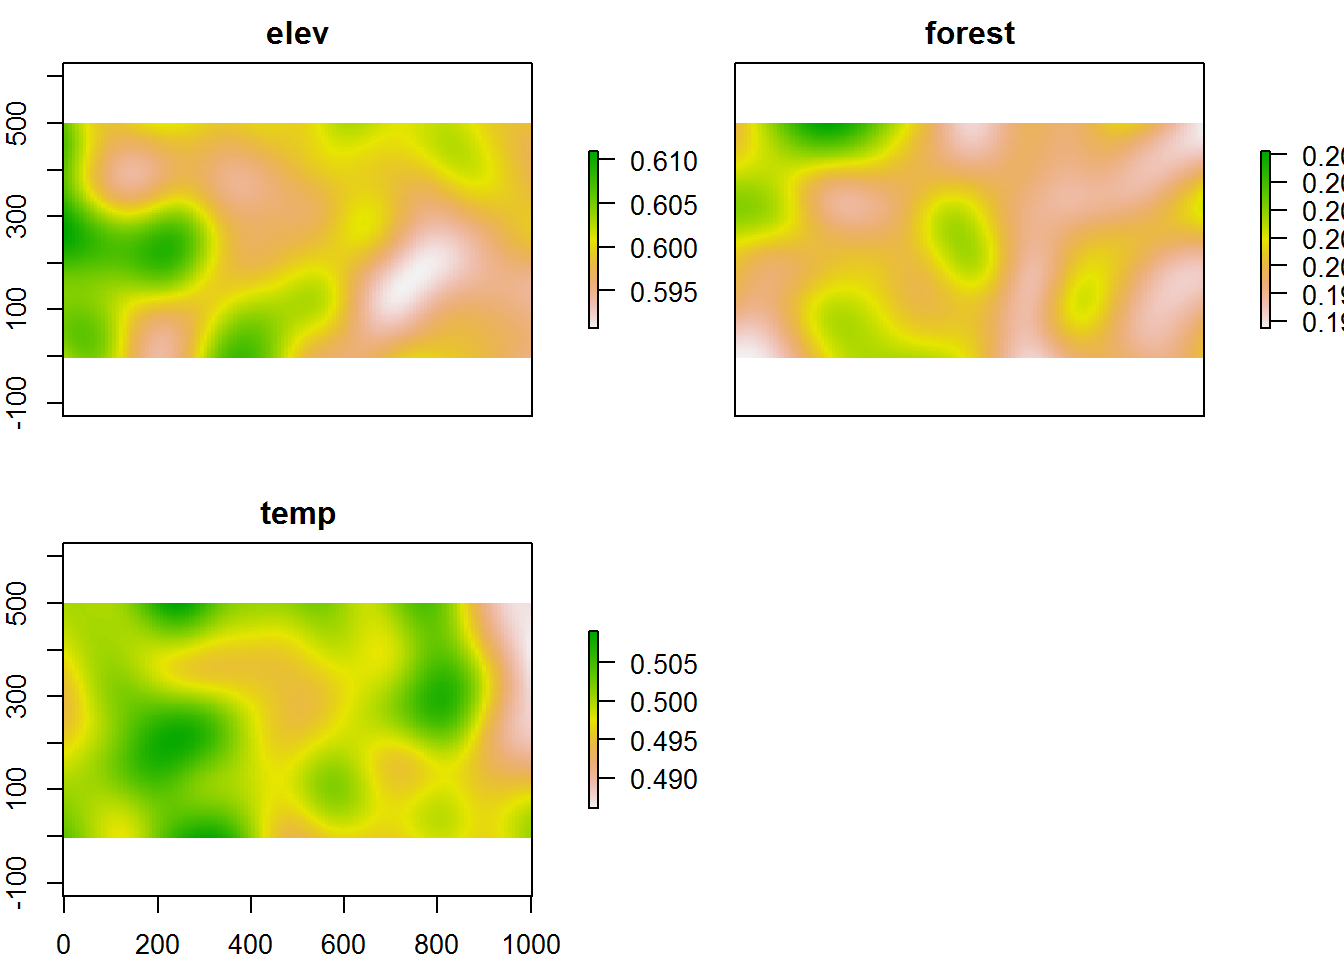
\includegraphics{Occu_Book_files/figure-latex/spat-1} \caption[fig]{Simulated map of elevation, forest and temperature.}\label{fig:spat}
\end{figure}

Once we have our covariate maps, we use them to predict with the best model. In this way we can have a map with predictions of the occupancy and the probability of detection.

\begin{Shaded}
\begin{Highlighting}[]
\CommentTok{\# make the predictions }
\NormalTok{predictions\_psi }\OtherTok{\textless{}{-}} \FunctionTok{predict}\NormalTok{(fm7, }\AttributeTok{type=}\StringTok{"state"}\NormalTok{, }\AttributeTok{newdata=}\NormalTok{mapdata.m) }\CommentTok{\# predict psi}
\end{Highlighting}
\end{Shaded}

\begin{verbatim}
##   doing row 1000 of 16384 
##   doing row 2000 of 16384 
##   doing row 3000 of 16384 
##   doing row 4000 of 16384 
##   doing row 5000 of 16384 
##   doing row 6000 of 16384 
##   doing row 7000 of 16384 
##   doing row 8000 of 16384 
##   doing row 9000 of 16384 
##   doing row 10000 of 16384 
##   doing row 11000 of 16384 
##   doing row 12000 of 16384 
##   doing row 13000 of 16384 
##   doing row 14000 of 16384 
##   doing row 15000 of 16384 
##   doing row 16000 of 16384
\end{verbatim}

\begin{Shaded}
\begin{Highlighting}[]
\NormalTok{predictions\_p   }\OtherTok{\textless{}{-}} \FunctionTok{predict}\NormalTok{(fm7, }\AttributeTok{type=}\StringTok{"det"}\NormalTok{,   }\AttributeTok{newdata=}\NormalTok{mapdata.m) }\CommentTok{\# predict p}
\end{Highlighting}
\end{Shaded}

\begin{verbatim}
##   doing row 1000 of 16384 
##   doing row 2000 of 16384 
##   doing row 3000 of 16384 
##   doing row 4000 of 16384 
##   doing row 5000 of 16384 
##   doing row 6000 of 16384 
##   doing row 7000 of 16384 
##   doing row 8000 of 16384 
##   doing row 9000 of 16384 
##   doing row 10000 of 16384 
##   doing row 11000 of 16384 
##   doing row 12000 of 16384 
##   doing row 13000 of 16384 
##   doing row 14000 of 16384 
##   doing row 15000 of 16384 
##   doing row 16000 of 16384
\end{verbatim}

\begin{Shaded}
\begin{Highlighting}[]
\CommentTok{\# put in the same stack}
\NormalTok{predmaps}\OtherTok{\textless{}{-}}\FunctionTok{stack}\NormalTok{(predictions\_psi}\SpecialCharTok{$}\NormalTok{Predicted,predictions\_p}\SpecialCharTok{$}\NormalTok{Predicted) }
\FunctionTok{names}\NormalTok{(predmaps)}\OtherTok{\textless{}{-}}\FunctionTok{c}\NormalTok{(}\StringTok{"psi\_predicted"}\NormalTok{, }\StringTok{"p\_predicted"}\NormalTok{) }\CommentTok{\# put names}
\FunctionTok{plot}\NormalTok{(predmaps)}
\end{Highlighting}
\end{Shaded}

\begin{figure}
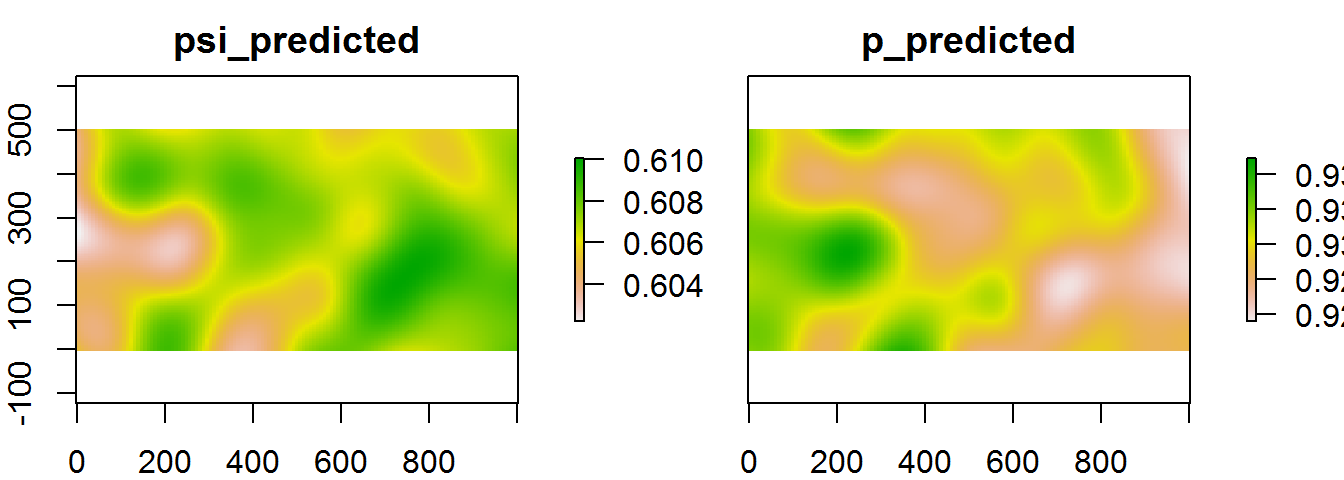
\includegraphics{Occu_Book_files/figure-latex/spatr-1} \caption[fig.]{Spatially explicit detection and occupancy models.}\label{fig:spatr}
\end{figure}

\hypertarget{bayesian}{%
\chapter{Bayesian analysis}\label{bayesian}}

In this part we are going to estimate the same parameters of a model equal to the ``best model'' which was selected in the unmarked model selection procedure in the previous chapter. Recall that this model has beta1 and alpha1, alpha2, alpha3. The parameters that we will estimate with the Bayesian method are going to be compared with the parameters that we already estimated with ML in unmarked and we will also compare them with the real parameters that we defined when establishing the data (data2) with the function data.fn, to see which of the two estimation methods (ML or Bayesian) are closer to the real parameters.

\hypertarget{generating-the-data-1}{%
\section{Generating the data}\label{generating-the-data-1}}

Again we will use a TEAM-type design (\url{https://www.wildlifeinsights.org/team-network}) with 60 sampling sites and 30 repeated visits, which is equivalent to the 30 days that the cameras remain active in the field. Our species remains the same, the white-tailed deer. For this example we will assume that detection is 0.6, occupancy is 0.8, and the interactions are simple with altitude as the only covariate explaining occupancy. But for detection there is a more complex relationship, assuming there is a slight interaction between the observation covariates. For observation, altitude and temperature interact with each other. Also note how altitude influences in opposite directions with a positive altitude sign for detection and a negative sign for occupancy.

\begin{Shaded}
\begin{Highlighting}[]
\CommentTok{\# }\AlertTok{\#\#\#}\CommentTok{ Generate a new data set or use the same}
\CommentTok{\# \# ****************************************}
\CommentTok{\# set.seed(148)}
\CommentTok{\# data \textless{}{-} data.fn(show.plot = T)    \# Default arguments}
\CommentTok{\# str(data)                         \# Look at the object}
\CommentTok{\# we are oing to use the data from datos2 object}

\DocumentationTok{\#\#\# Fit same model with JAGS, using library jagsUI}
\CommentTok{\# ************************************************}
\CommentTok{\# Bundle data}
\NormalTok{win.data }\OtherTok{\textless{}{-}} \FunctionTok{list}\NormalTok{(}\AttributeTok{y =}\NormalTok{ datos2}\SpecialCharTok{$}\NormalTok{y, }
                 \AttributeTok{M =} \FunctionTok{nrow}\NormalTok{(datos2}\SpecialCharTok{$}\NormalTok{y), }
                 \AttributeTok{J =} \FunctionTok{ncol}\NormalTok{(datos2}\SpecialCharTok{$}\NormalTok{y), }
                 \AttributeTok{elev =}\NormalTok{ datos2}\SpecialCharTok{$}\NormalTok{elev, }
                 \AttributeTok{forest =}\NormalTok{ datos2}\SpecialCharTok{$}\NormalTok{forest, }
                 \AttributeTok{temp =}\NormalTok{ datos2}\SpecialCharTok{$}\NormalTok{temp)}
\CommentTok{\# str(win.data)}


\CommentTok{\# \# Specify model in BUGS language}
\CommentTok{\# sink("model22.txt")}
\CommentTok{\# cat("}
\CommentTok{\# model \{}
\CommentTok{\# }
\CommentTok{\# \# Priors}
\CommentTok{\# mean.p \textasciitilde{} dunif(0, 1)        \# Detection intercept on prob. scale}
\CommentTok{\# alpha0 \textless{}{-} logit(mean.p)     \# same on logit scale}
\CommentTok{\# mean.psi \textasciitilde{} dunif(0, 1)      \# Occupancy intercept on prob. scale}
\CommentTok{\# beta0 \textless{}{-} logit(mean.psi)    \# same on logit scale}
\CommentTok{\# for(k in 1:3)\{              \# 2 detection covariates + 1 interact}
\CommentTok{\#     alpha[k] \textasciitilde{} dnorm(0, 0.01) \# Covariates on logit(detection)}
\CommentTok{\# \#   alpha[k] \textasciitilde{} dnorm(0, 0.05) \# Covariates on logit(detection)}
\CommentTok{\# \#   alpha[k] \textasciitilde{} dunif({-}10, 10) \# Covariates on logit(detection)}
\CommentTok{\# \}}
\CommentTok{\# }
\CommentTok{\# for(k in 1:1)\{                \# 2 occupancy covariates + 1 interact}
\CommentTok{\#     beta[k] \textasciitilde{} dnorm(0, 0.01)  \# Covariates on logit(occupancy)}
\CommentTok{\# \#   beta[k] \textasciitilde{} dnorm(0, 0.05)  \# Covariates on logit(occupancy)}
\CommentTok{\# \#   beta[k] \textasciitilde{} dunif({-}10, 10)  \# Covariates on logit(occupancy)}
\CommentTok{\# \}}
\CommentTok{\# }
\CommentTok{\# \# Translation of the occupancy parameters in unmarked into those for BUGS:}
\CommentTok{\# \# (Intercept)         (beta0 in BUGS)}
\CommentTok{\# \# elev                (beta[1])}
\CommentTok{\# \# forest              (beta[2])}
\CommentTok{\# \# temp                (beta[3])}
\CommentTok{\# \# elev:forest         (beta[4])}
\CommentTok{\# \# elev:temp           (beta[5])}
\CommentTok{\# \# forest:temp         (beta[6])}
\CommentTok{\# \# elev:forest:temp    (beta[7])}
\CommentTok{\# }
\CommentTok{\# }
\CommentTok{\# \# Likelihood}
\CommentTok{\# for (i in 1:M) \{}
\CommentTok{\#   \# True state model for the partially observed true state}
\CommentTok{\#   z[i] \textasciitilde{} dbern(psi[i])                      \# True occupancy z at site i}
\CommentTok{\#   logit(psi[i]) \textless{}{-} beta0 +                  \# occupancy (psi) intercept}
\CommentTok{\#     beta[1] * elev[i] \#+                     \# elev}
\CommentTok{\#     \#beta[2] * forest[i] \#+                  \# forest}
\CommentTok{\#     \#beta[3] * elev[i] * forest[i]          \# elev:forest}
\CommentTok{\#     \#beta[4] * elev[i] * temp[i] +          \# elev:temp}
\CommentTok{\#     \#beta[5] * temp[i] +                    \# temp}
\CommentTok{\#     \#beta[6] * forest[i] * temp[i] +        \# forest:temp}
\CommentTok{\#     \#beta[7] * elev[i] * forest[i] * temp[i]   \# elev:forest:temp}
\CommentTok{\# }
\CommentTok{\#    for (j in 1:J) \{}
\CommentTok{\#       \# Observation model for the actual observations}
\CommentTok{\#       y[i,j] \textasciitilde{} dbern(p.eff[i,j])      \# Detection{-}nondetection at i and j}
\CommentTok{\#       p.eff[i,j] \textless{}{-} z[i] * p[i,j]}
\CommentTok{\#       logit(p[i,j]) \textless{}{-} alpha0 +             \# detection (p) intercept}
\CommentTok{\#          alpha[1] * elev[i] +               \# effect of elevation on p}
\CommentTok{\#          alpha[2] * temp[i,j] +             \# effect of temp on p}
\CommentTok{\#          alpha[3] * elev[i] * temp[i,j]     \# effect of elev:temp on p}
\CommentTok{\#    \}}
\CommentTok{\# \}}
\CommentTok{\# }
\CommentTok{\# \# Derived quantities}
\CommentTok{\# sumZ \textless{}{-} sum(z[])      \# Number of occupied sites among those studied}
\CommentTok{\# occ.fs \textless{}{-} sum(z[])/M  \# proportion of occupied sites among those studied}
\CommentTok{\# logit.psi \textless{}{-} beta0    \# For comparison with unmarked}
\CommentTok{\# logit.p \textless{}{-} alpha0     \# For comparison with unmarked}
\CommentTok{\# \}}
\CommentTok{\# ",fill = TRUE)}
\CommentTok{\# sink()}


\FunctionTok{library}\NormalTok{(jagsUI)}
\CommentTok{\# library(R2jags)}
\CommentTok{\# Initial values}
\NormalTok{zst }\OtherTok{\textless{}{-}} \FunctionTok{apply}\NormalTok{(datos2}\SpecialCharTok{$}\NormalTok{y, }\DecValTok{1}\NormalTok{, max)}
\NormalTok{inits }\OtherTok{\textless{}{-}} \ControlFlowTok{function}\NormalTok{()\{}\FunctionTok{list}\NormalTok{(}\AttributeTok{z =}\NormalTok{ zst, }
                         \AttributeTok{mean.psi =} \FunctionTok{runif}\NormalTok{(}\DecValTok{1}\NormalTok{), }
                         \AttributeTok{mean.p =} \FunctionTok{runif}\NormalTok{(}\DecValTok{1}\NormalTok{), }
                         \AttributeTok{alpha =} \FunctionTok{rnorm}\NormalTok{(}\DecValTok{3}\NormalTok{), }\CommentTok{\# adjust here}
                         \AttributeTok{beta =} \FunctionTok{rnorm}\NormalTok{(}\DecValTok{1}\NormalTok{))\} }\CommentTok{\# adjust here}

\CommentTok{\# Parameters monitored}
\NormalTok{params }\OtherTok{\textless{}{-}} \FunctionTok{c}\NormalTok{(}\StringTok{"sumZ"}\NormalTok{, }\StringTok{"occ.fs"}\NormalTok{, }\StringTok{"logit.psi"}\NormalTok{, }\StringTok{"logit.p"}\NormalTok{, }\StringTok{"alpha"}\NormalTok{, }\StringTok{"beta"}\NormalTok{)}

\CommentTok{\# MCMC settings}
\CommentTok{\# ni \textless{}{-} 100000   ;   nt \textless{}{-} 10   ;   nb \textless{}{-} 1000   ;   nc \textless{}{-} 3}
\NormalTok{ ni }\OtherTok{\textless{}{-}} \DecValTok{10000}\NormalTok{   ;   nt }\OtherTok{\textless{}{-}} \DecValTok{10}\NormalTok{   ;   nb }\OtherTok{\textless{}{-}} \DecValTok{500}\NormalTok{   ;   nc }\OtherTok{\textless{}{-}} \DecValTok{3}

\CommentTok{\# Call JAGS from R (ART 260 sec with norm(), 480 with unif({-}10,10)) }
\CommentTok{\# and summarize posteriors}
\FunctionTok{system.time}\NormalTok{(out22 }\OtherTok{\textless{}{-}} \FunctionTok{jags}\NormalTok{(win.data, inits, }\AttributeTok{parameters.to.save =}\NormalTok{ params,}
                      \AttributeTok{model.file =} \StringTok{"D:/BoxFiles/Box Sync/CodigoR/Toshiba/IntroOccuBook/bookdown{-}demo{-}master/model22.txt"}\NormalTok{, }
                          \AttributeTok{n.chains =}\NormalTok{ nc, }
                          \AttributeTok{n.thin =}\NormalTok{ nt, }
                          \AttributeTok{n.iter =}\NormalTok{ ni, }
                          \AttributeTok{n.burnin =}\NormalTok{ nb, }
                          \AttributeTok{parallel =}\NormalTok{ T))}
\end{Highlighting}
\end{Shaded}

\begin{verbatim}
## 
## Processing function input....... 
## 
## Done. 
##  
## Beginning parallel processing using 3 cores. Console output will be suppressed.
## 
## Parallel processing completed.
## 
## Calculating statistics....... 
## 
## Done.
\end{verbatim}

\begin{verbatim}
##    user  system elapsed 
##    0.03    0.00  253.36
\end{verbatim}

\begin{Shaded}
\begin{Highlighting}[]
\CommentTok{\# See model diagnistics and convergence }
\FunctionTok{library}\NormalTok{(mcmcplots)}
\FunctionTok{library}\NormalTok{(ggmcmc)}
\NormalTok{fit22.mcmc }\OtherTok{\textless{}{-}} \FunctionTok{as.mcmc.list}\NormalTok{(out22}\SpecialCharTok{$}\NormalTok{samples)}
\NormalTok{bayes.mod.fit.gg }\OtherTok{\textless{}{-}} \FunctionTok{ggs}\NormalTok{(fit22.mcmc) }\CommentTok{\#convert to ggmcmc}
\FunctionTok{ggs\_running}\NormalTok{(bayes.mod.fit.gg)}\CommentTok{\# check if chains approach target distrib. }
\end{Highlighting}
\end{Shaded}

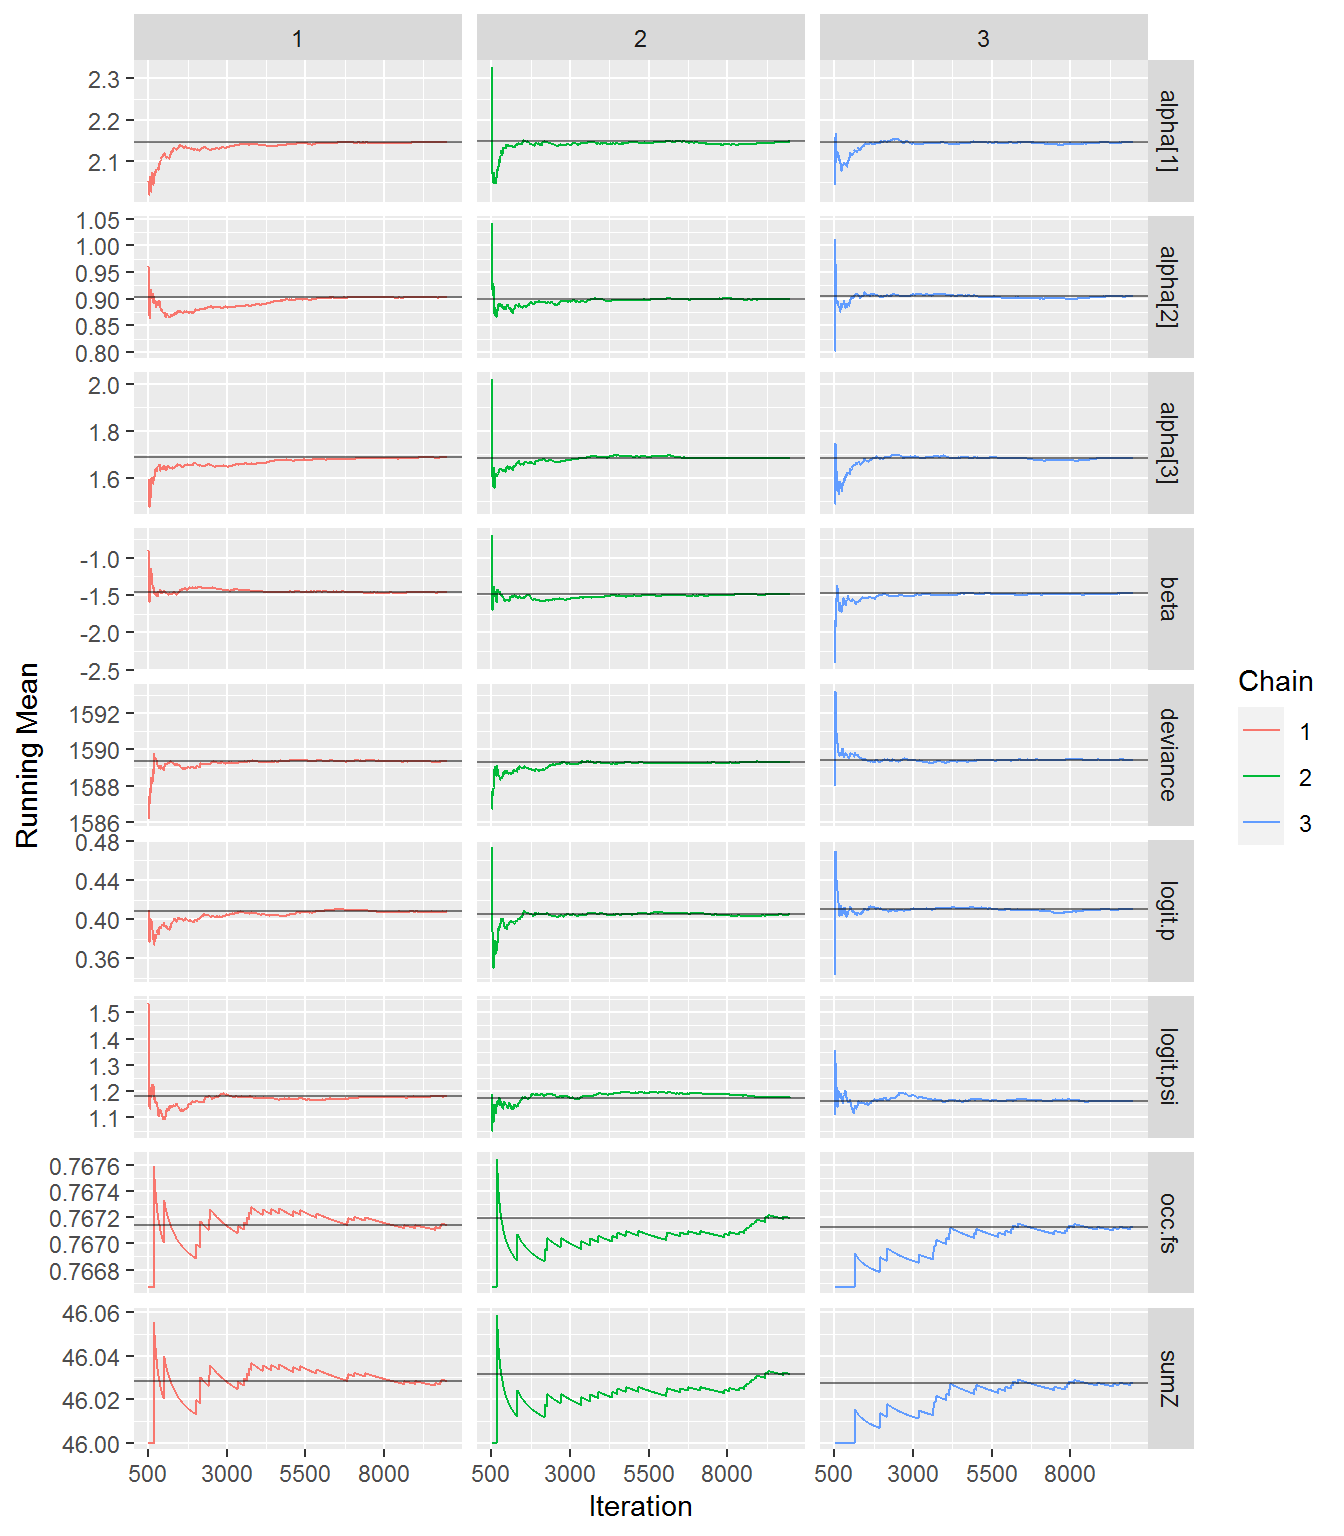
\includegraphics{Occu_Book_files/figure-latex/bayesian-1.pdf}

\begin{Shaded}
\begin{Highlighting}[]
\CommentTok{\# denplot(fit22.mcmc, parms = c("beta", }
\CommentTok{\#                               "alpha[1]", "alpha[2]", "alpha[3]", }
\CommentTok{\#                               "logit.psi", "logit.p" ))}
\CommentTok{\# traplot(fit22.mcmc)}
\CommentTok{\# ggs\_density(bayes.mod.fit.gg)}

\CommentTok{\# xyplot(out22)        \# assess within{-}chain convergence}
\FunctionTok{densityplot}\NormalTok{(out22)  }\CommentTok{\# shape of the posterior distribution}
\end{Highlighting}
\end{Shaded}

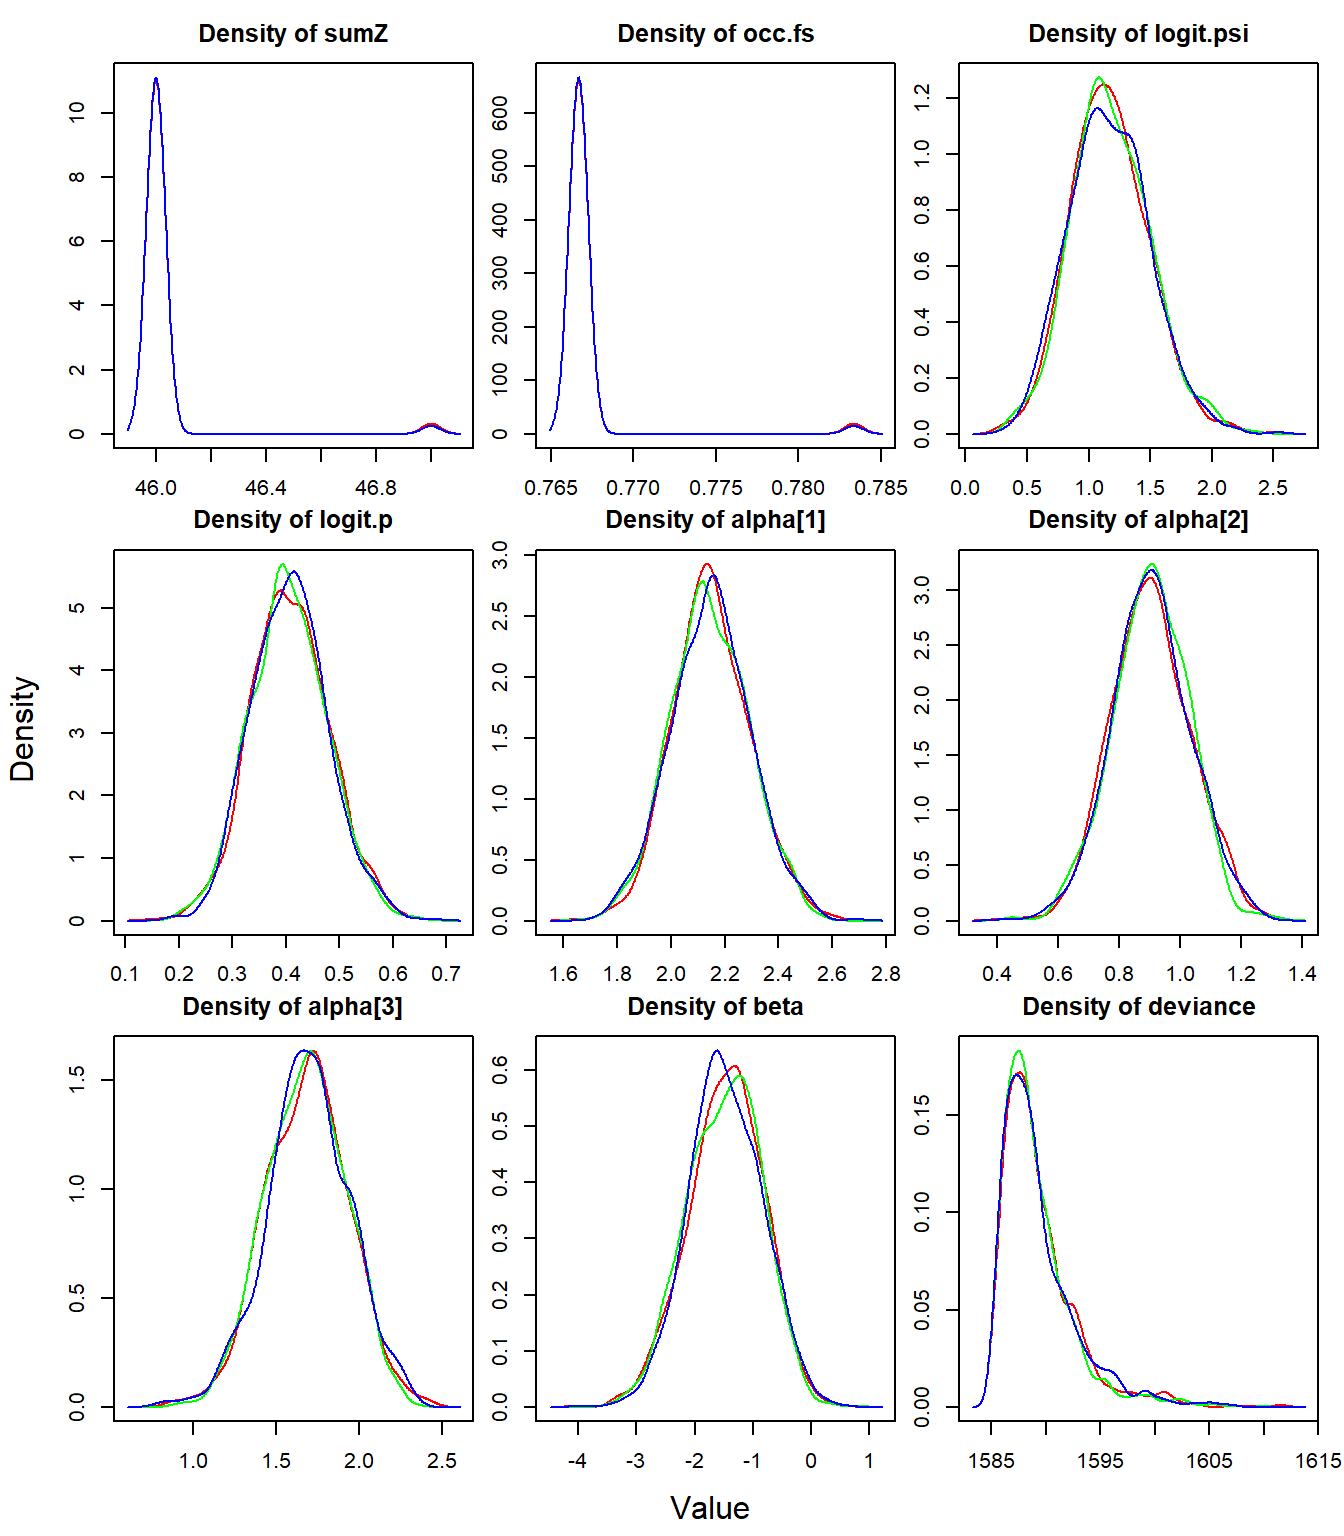
\includegraphics{Occu_Book_files/figure-latex/bayesian-2.pdf}

\begin{Shaded}
\begin{Highlighting}[]
\CommentTok{\# see model result and estimates  }
\FunctionTok{print}\NormalTok{(out22, }\DecValTok{3}\NormalTok{)}
\end{Highlighting}
\end{Shaded}

\begin{verbatim}
## JAGS output for model 'D:/BoxFiles/Box Sync/CodigoR/Toshiba/IntroOccuBook/bookdown-demo-master/model22.txt', generated by jagsUI.
## Estimates based on 3 chains of 10000 iterations,
## adaptation = 100 iterations (sufficient),
## burn-in = 500 iterations and thin rate = 10,
## yielding 2850 total samples from the joint posterior. 
## MCMC ran in parallel for 4.222 minutes at time 2022-06-26 00:36:52.
## 
##               mean    sd     2.5%
## sumZ        46.029 0.168   46.000
## occ.fs       0.767 0.003    0.767
## logit.psi    1.173 0.324    0.562
## logit.p      0.408 0.074    0.263
## alpha[1]     2.147 0.152    1.853
## alpha[2]     0.902 0.126    0.657
## alpha[3]     1.686 0.247    1.208
## beta        -1.475 0.632   -2.769
## deviance  1589.362 3.508 1585.504
##                50%    97.5% overlap0
## sumZ        46.000   47.000    FALSE
## occ.fs       0.767    0.783    FALSE
## logit.psi    1.163    1.825    FALSE
## logit.p      0.407    0.560    FALSE
## alpha[1]     2.143    2.445    FALSE
## alpha[2]     0.903    1.155    FALSE
## alpha[3]     1.682    2.180    FALSE
## beta        -1.458   -0.329    FALSE
## deviance  1588.480 1599.696    FALSE
##               f  Rhat n.eff
## sumZ      1.000 1.000  2850
## occ.fs    1.000 1.000  2850
## logit.psi 1.000 1.000  2850
## logit.p   1.000 1.001  2372
## alpha[1]  1.000 1.000  2850
## alpha[2]  1.000 1.000  2850
## alpha[3]  1.000 1.000  2850
## beta      0.995 1.000  2850
## deviance  1.000 1.000  2850
## 
## Successful convergence based on Rhat values (all < 1.1). 
## Rhat is the potential scale reduction factor (at convergence, Rhat=1). 
## For each parameter, n.eff is a crude measure of effective sample size. 
## 
## overlap0 checks if 0 falls in the parameter's 95% credible interval.
## f is the proportion of the posterior with the same sign as the mean;
## i.e., our confidence that the parameter is positive or negative.
## 
## DIC info: (pD = var(deviance)/2) 
## pD = 6.2 and DIC = 1595.517 
## DIC is an estimate of expected predictive error (lower is better).
\end{verbatim}

\begin{Shaded}
\begin{Highlighting}[]
\CommentTok{\# store in tmp coefficients from best ML model}
\NormalTok{tmp }\OtherTok{\textless{}{-}} \FunctionTok{summary}\NormalTok{(fm7)}
\end{Highlighting}
\end{Shaded}

\begin{verbatim}
## 
## Call:
## occu(formula = ~elev + temp + elev:temp ~ elev, data = umf)
## 
## Occupancy (logit-scale):
##             Estimate    SE     z  P(>|z|)
## (Intercept)     1.18 0.326  3.62 0.000291
## elev           -1.41 0.624 -2.26 0.023548
## 
## Detection (logit-scale):
##             Estimate     SE     z
## (Intercept)    0.407 0.0735  5.54
## elev           2.140 0.1494 14.32
## temp           0.900 0.1262  7.14
## elev:temp      1.680 0.2514  6.68
##              P(>|z|)
## (Intercept) 3.03e-08
## elev        1.66e-46
## temp        9.68e-13
## elev:temp   2.34e-11
## 
## AIC: 1656.533 
## Number of sites: 60
## optim convergence code: 0
## optim iterations: 38 
## Bootstrap iterations: 0
\end{verbatim}

\begin{Shaded}
\begin{Highlighting}[]
\NormalTok{modestimates }\OtherTok{\textless{}{-}} \FunctionTok{cbind}\NormalTok{(}\FunctionTok{rbind}\NormalTok{(tmp}\SpecialCharTok{$}\NormalTok{state[}\DecValTok{1}\SpecialCharTok{:}\DecValTok{2}\NormalTok{], tmp}\SpecialCharTok{$}\NormalTok{det[}\DecValTok{1}\SpecialCharTok{:}\DecValTok{2}\NormalTok{]), }
                \AttributeTok{Post.mean =}\NormalTok{ out22}\SpecialCharTok{$}\NormalTok{summary[}\FunctionTok{c}\NormalTok{(}\DecValTok{3}\NormalTok{, }\DecValTok{8}\NormalTok{, }\DecValTok{4}\SpecialCharTok{:}\DecValTok{7}\NormalTok{), }\DecValTok{1}\NormalTok{],}
                \AttributeTok{Post.sd   =}\NormalTok{ out22}\SpecialCharTok{$}\NormalTok{summary[}\FunctionTok{c}\NormalTok{(}\DecValTok{3}\NormalTok{, }\DecValTok{8}\NormalTok{, }\DecValTok{4}\SpecialCharTok{:}\DecValTok{7}\NormalTok{), }\DecValTok{2}\NormalTok{] )}

\CommentTok{\# fix the(logit{-}scale) in unmarked }
\NormalTok{modestimates[}\DecValTok{1}\NormalTok{,}\DecValTok{1}\NormalTok{]}\OtherTok{\textless{}{-}} \FunctionTok{plogis}\NormalTok{(modestimates[}\DecValTok{1}\NormalTok{,}\DecValTok{1}\NormalTok{])}
\NormalTok{modestimates[}\DecValTok{3}\NormalTok{,}\DecValTok{1}\NormalTok{]}\OtherTok{\textless{}{-}} \FunctionTok{plogis}\NormalTok{(modestimates[}\DecValTok{3}\NormalTok{,}\DecValTok{1}\NormalTok{])}

\CommentTok{\# fix the(logit{-}scale) in Bayes in logit.psi  logit.p}
\NormalTok{modestimates[}\DecValTok{1}\NormalTok{,}\DecValTok{3}\NormalTok{]}\OtherTok{\textless{}{-}} \FunctionTok{plogis}\NormalTok{(modestimates[}\DecValTok{1}\NormalTok{,}\DecValTok{3}\NormalTok{])}
\NormalTok{modestimates[}\DecValTok{3}\NormalTok{,}\DecValTok{3}\NormalTok{]}\OtherTok{\textless{}{-}} \FunctionTok{plogis}\NormalTok{(modestimates[}\DecValTok{3}\NormalTok{,}\DecValTok{3}\NormalTok{])}

\CommentTok{\# get real values from datos2 object}
\NormalTok{real}\OtherTok{\textless{}{-}} \FunctionTok{rbind}\NormalTok{(datos2}\SpecialCharTok{$}\NormalTok{mean.occupancy, datos2}\SpecialCharTok{$}\NormalTok{beta1, datos2}\SpecialCharTok{$}\NormalTok{mean.detection,}
\NormalTok{             datos2}\SpecialCharTok{$}\NormalTok{alpha1, datos2}\SpecialCharTok{$}\NormalTok{alpha2, datos2}\SpecialCharTok{$}\NormalTok{alpha3)}
\end{Highlighting}
\end{Shaded}

\hypertarget{comparing-the-actual-and-estimated-values-from-ml-and-bayesian}{%
\section{Comparing the actual and estimated values from ML and Bayesian}\label{comparing-the-actual-and-estimated-values-from-ml-and-bayesian}}

Let's see how close the estimates are to the actual values, by comparing the actual value with the Maximum Likelihood estimate (columns 2 and 3) and the Bayesian estimate (columns 4 and 5).

\begin{Shaded}
\begin{Highlighting}[]
\DocumentationTok{\#\#\# see if the values are close to real values}
\NormalTok{compare }\OtherTok{\textless{}{-}} \FunctionTok{cbind}\NormalTok{(real, modestimates) }\CommentTok{\# put both in same table}
\CommentTok{\# put names to rows}
\FunctionTok{rownames}\NormalTok{(compare) }\OtherTok{\textless{}{-}} \FunctionTok{c}\NormalTok{(}\StringTok{"psi"}\NormalTok{,}\StringTok{"beta"}\NormalTok{,}\StringTok{"p"}\NormalTok{,}\StringTok{"alpha1"}\NormalTok{,}\StringTok{"alpha2"}\NormalTok{, }\StringTok{"alpha3"}\NormalTok{)}

\CommentTok{\# print comparing table}
\FunctionTok{library}\NormalTok{(knitr)}
\FunctionTok{kable}\NormalTok{(compare)}
\end{Highlighting}
\end{Shaded}

\begin{tabular}{l|r|r|r|r|r}
\hline
  & real & Estimate & SE & Post.mean & Post.sd\\
\hline
psi & 0.8 & 0.7653197 & 0.3262574 & 0.7637476 & 0.3244823\\
\hline
beta & -1.5 & -1.4129006 & 0.6239572 & -1.4747848 & 0.6319201\\
\hline
p & 0.6 & 0.6004304 & 0.0735178 & 0.6005410 & 0.0744655\\
\hline
alpha1 & 2.0 & 2.1395071 & 0.1494144 & 2.1470247 & 0.1515634\\
\hline
alpha2 & 1.0 & 0.9003900 & 0.1261927 & 0.9021164 & 0.1257829\\
\hline
alpha3 & 1.5 & 1.6801587 & 0.2513946 & 1.6858529 & 0.2468270\\
\hline
\end{tabular}

\hypertarget{bayesian-estimates-easily-using-ubms}{%
\section{Bayesian estimates easily using ubms}\label{bayesian-estimates-easily-using-ubms}}

The JAGS code adds another layer of complexity to the analysis. Fortunately, since the year 2022, there is a new package in the neighborhood. The \href{https://kenkellner.com/ubms/}{ubms package} allows Bayesian estimates using the same easy and simple unmarked structure. The package has a formula-based interface compatible with unmarked, but the model is fit using MCMC with Stan instead of using maximum likelihood.

\begin{Shaded}
\begin{Highlighting}[]
\FunctionTok{library}\NormalTok{(ubms)}

\NormalTok{(fm7\_ubms }\OtherTok{\textless{}{-}} \FunctionTok{stan\_occu}\NormalTok{(}\SpecialCharTok{\textasciitilde{}}\NormalTok{ elev }\SpecialCharTok{+}\NormalTok{ temp }\SpecialCharTok{+}\NormalTok{ elev}\SpecialCharTok{:}\NormalTok{temp }\SpecialCharTok{\textasciitilde{}}\NormalTok{ elev, umf, }\AttributeTok{chains=}\DecValTok{3}\NormalTok{, }\AttributeTok{cores=}\DecValTok{3}\NormalTok{))}
\end{Highlighting}
\end{Shaded}

\begin{verbatim}
## 
## Call:
## stan_occu(formula = ~elev + temp + elev:temp ~ elev, data = umf, 
##     chains = 3, cores = 3)
## 
## Occupancy (logit-scale):
##             Estimate    SD   2.5%  97.5%
## (Intercept)     1.16 0.325  0.567  1.812
## elev           -1.27 0.568 -2.447 -0.223
##             n_eff  Rhat
## (Intercept)  3548 1.000
## elev         2970 0.999
## 
## Detection (logit-scale):
##             Estimate     SD  2.5% 97.5%
## (Intercept)    0.398 0.0742 0.257 0.555
## elev           2.117 0.1481 1.825 2.419
## temp           0.882 0.1272 0.633 1.134
## elev:temp      1.627 0.2514 1.129 2.147
##             n_eff Rhat
## (Intercept)  3054    1
## elev         2670    1
## temp         2931    1
## elev:temp    3109    1
## 
## LOOIC: 1657.562
## Runtime: 6.163 sec
\end{verbatim}

\begin{Shaded}
\begin{Highlighting}[]
\CommentTok{\# Assess model goodness{-}of{-}fit with a posterior predictive check, using the MacKenzie{-}Bailey chi{-}square test:}
\NormalTok{fm\_fit }\OtherTok{\textless{}{-}} \FunctionTok{gof}\NormalTok{(fm7\_ubms, }\AttributeTok{draws=}\DecValTok{500}\NormalTok{)}
\FunctionTok{plot}\NormalTok{(fm\_fit)}
\end{Highlighting}
\end{Shaded}

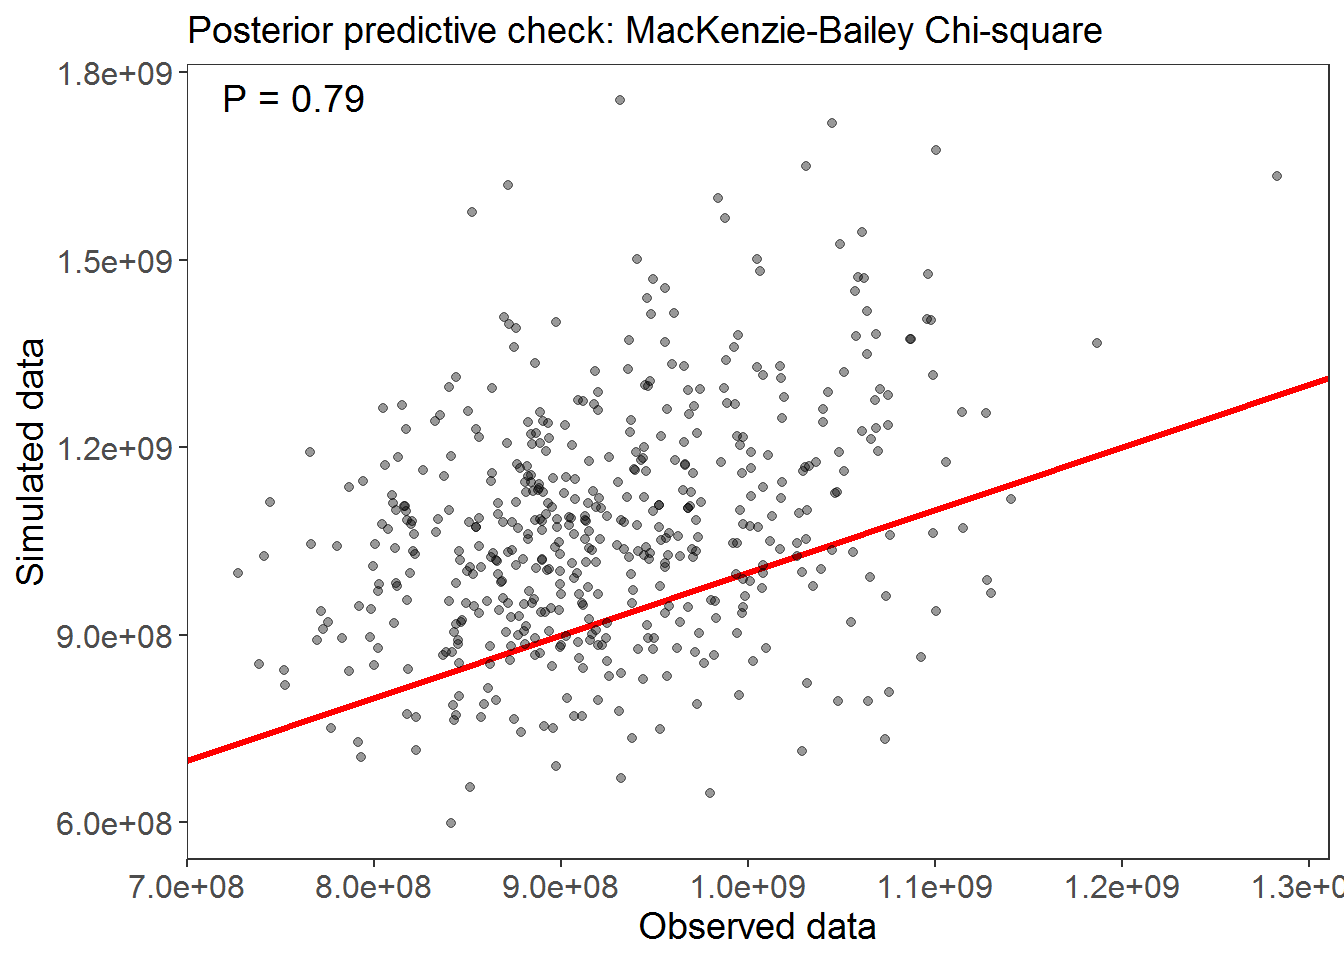
\includegraphics{Occu_Book_files/figure-latex/ubms_umf1_ch7-1.pdf}

\begin{Shaded}
\begin{Highlighting}[]
\CommentTok{\# Look at the marginal effect of on detection:}

\FunctionTok{plot\_effects}\NormalTok{(fm7\_ubms, }\StringTok{"det"}\NormalTok{)}
\end{Highlighting}
\end{Shaded}

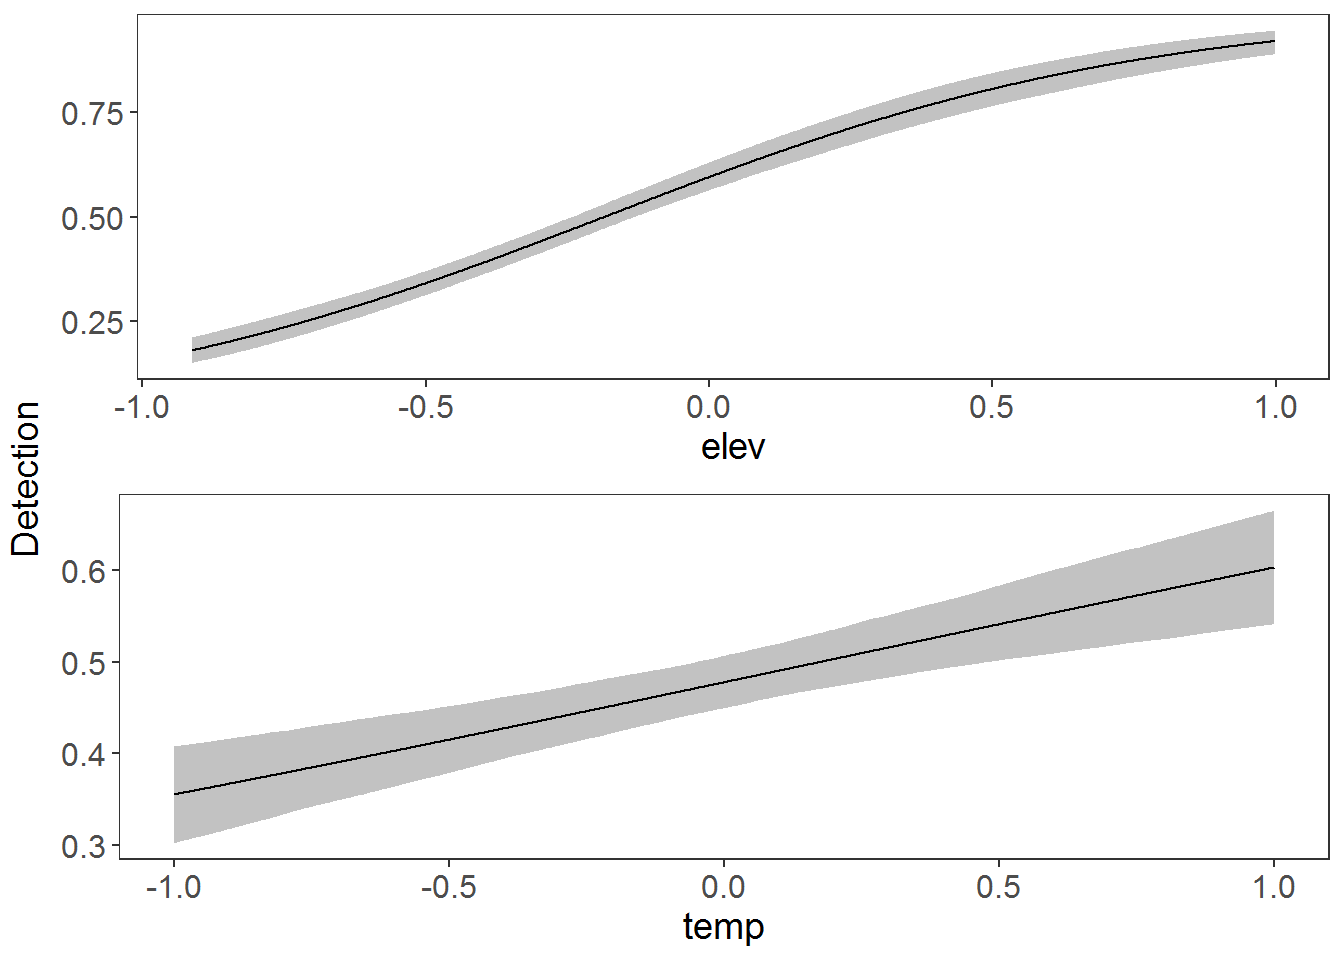
\includegraphics{Occu_Book_files/figure-latex/ubms_umf1_ch7-2.pdf}

\begin{Shaded}
\begin{Highlighting}[]
\CommentTok{\# Look at the marginal effect of on Occupancy:}

\FunctionTok{plot\_effects}\NormalTok{(fm7\_ubms, }\StringTok{"state"}\NormalTok{)}
\end{Highlighting}
\end{Shaded}

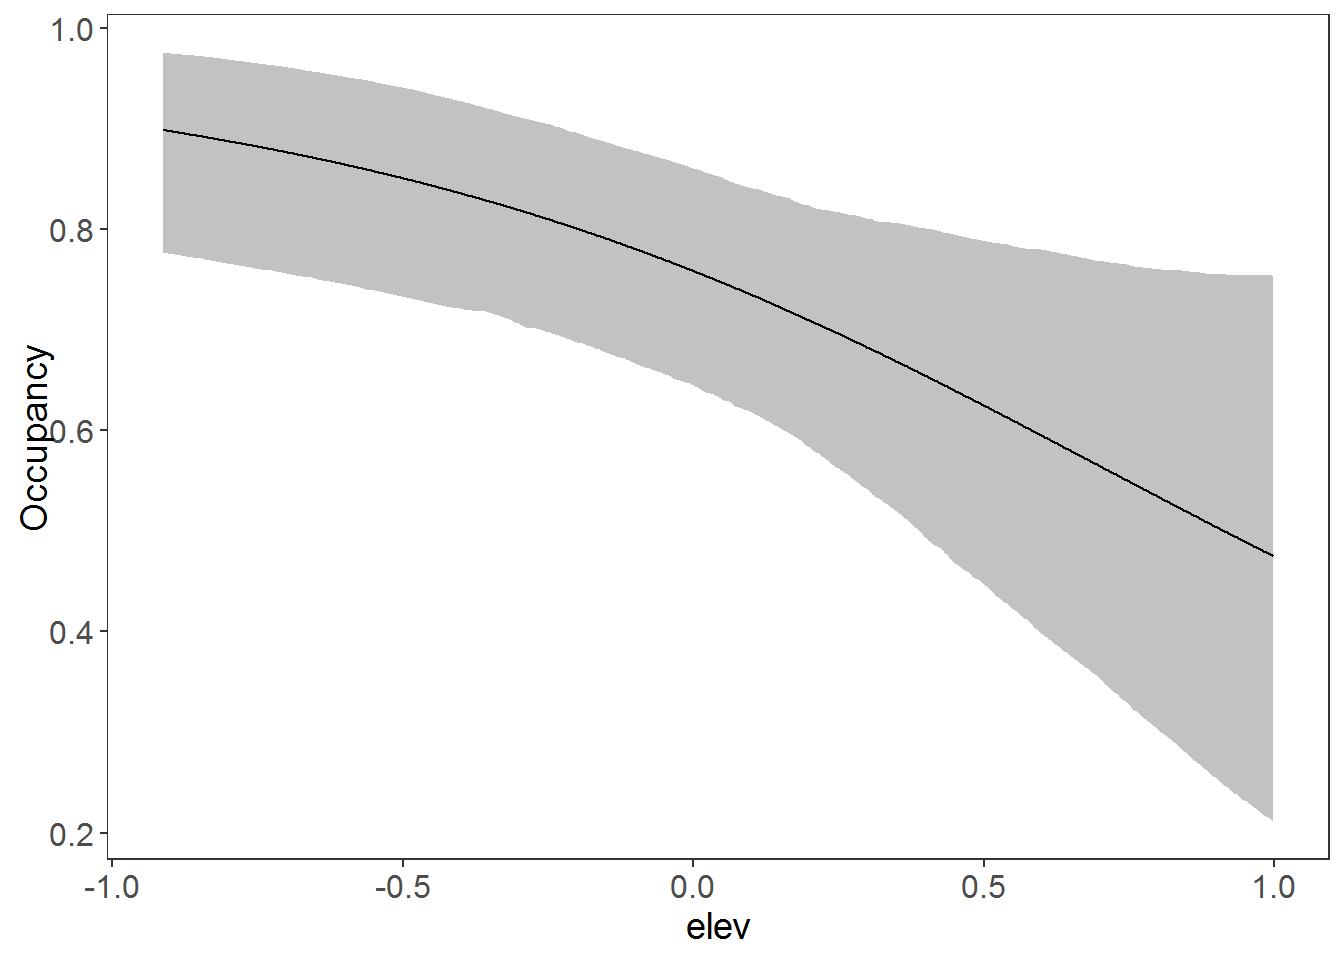
\includegraphics{Occu_Book_files/figure-latex/ubms_umf1_ch7-3.pdf}

\hypertarget{advantages-of-ubms-compared-to-unmarked}{%
\subsection{Advantages of ubms compared to unmarked:}\label{advantages-of-ubms-compared-to-unmarked}}

\begin{enumerate}
\def\labelenumi{\arabic{enumi}.}
\item
  Obtain posterior distributions of parameters and derived parameters.
\item
  Include random effects in parameter formulas (same syntax as lme4).
\item
  Assess model fit using WAIC and LOO via the loo package.
\end{enumerate}

\hypertarget{disadvantages-of-ubms-compared-to-unmarked}{%
\subsection{Disadvantages of ubms compared to unmarked:}\label{disadvantages-of-ubms-compared-to-unmarked}}

\begin{enumerate}
\def\labelenumi{\arabic{enumi}.}
\item
  MCMC is slower than maximum likelihood.
\item
  Not all model types are supported.
\item
  Potential for convergence issues
\end{enumerate}

\hypertarget{r-session-information-and-packages-used}{%
\chapter{R session information and packages used}\label{r-session-information-and-packages-used}}

\begin{Shaded}
\begin{Highlighting}[]
\FunctionTok{sessionInfo}\NormalTok{()}
\end{Highlighting}
\end{Shaded}

\begin{verbatim}
## R version 4.0.3 (2020-10-10)
## Platform: x86_64-w64-mingw32/x64 (64-bit)
## Running under: Windows 10 x64 (build 14393)
## 
## Matrix products: default
## 
## locale:
## [1] LC_COLLATE=Spanish_Colombia.1252 
## [2] LC_CTYPE=Spanish_Colombia.1252   
## [3] LC_MONETARY=Spanish_Colombia.1252
## [4] LC_NUMERIC=C                     
## [5] LC_TIME=Spanish_Colombia.1252    
## 
## attached base packages:
## [1] stats     graphics  grDevices
## [4] utils     datasets  methods  
## [7] base     
## 
## other attached packages:
##  [1] ggmcmc_1.5.1.1       
##  [2] ggplot2_3.3.6        
##  [3] tidyr_1.1.4          
##  [4] dplyr_1.0.7          
##  [5] mcmcplots_0.4.3      
##  [6] coda_0.19-4          
##  [7] jagsUI_1.5.2         
##  [8] spatstat_2.2-0       
##  [9] spatstat.linnet_2.3-0
## [10] spatstat.core_2.3-0  
## [11] rpart_4.1-15         
## [12] nlme_3.1-152         
## [13] spatstat.geom_2.2-2  
## [14] spatstat.data_2.1-0  
## [15] raster_3.5-15        
## [16] sp_1.4-5             
## [17] knitr_1.39           
## [18] bookdown_0.24        
## [19] ubms_1.1.0           
## [20] unmarked_1.1.1       
## [21] lattice_0.20-44      
## 
## loaded via a namespace (and not attached):
##  [1] spatstat.sparse_2.0-0
##  [2] matrixStats_0.62.0   
##  [3] RColorBrewer_1.1-3   
##  [4] rstan_2.26.10        
##  [5] tools_4.0.3          
##  [6] bslib_0.2.5.1        
##  [7] utf8_1.2.2           
##  [8] R6_2.5.1             
##  [9] mgcv_1.8-36          
## [10] DBI_1.1.2            
## [11] colorspace_2.0-3     
## [12] withr_2.5.0          
## [13] GGally_2.1.2         
## [14] tidyselect_1.1.1     
## [15] gridExtra_2.3        
## [16] prettyunits_1.1.1    
## [17] processx_3.5.3       
## [18] curl_4.3.2           
## [19] compiler_4.0.3       
## [20] cli_3.2.0            
## [21] denstrip_1.5.4       
## [22] labeling_0.4.2       
## [23] sass_0.4.0           
## [24] sfsmisc_1.1-11       
## [25] scales_1.2.0         
## [26] callr_3.7.0          
## [27] pbapply_1.5-0        
## [28] askpass_1.1          
## [29] goftest_1.2-2        
## [30] stringr_1.4.0        
## [31] digest_0.6.29        
## [32] StanHeaders_2.26.10  
## [33] spatstat.utils_2.2-0 
## [34] minqa_1.2.4          
## [35] rmarkdown_2.14       
## [36] pkgconfig_2.0.3      
## [37] htmltools_0.5.1.1    
## [38] lme4_1.1-29          
## [39] highr_0.9            
## [40] rlang_1.0.2          
## [41] rstudioapi_0.13      
## [42] jquerylib_0.1.4      
## [43] farver_2.1.0         
## [44] generics_0.1.2       
## [45] jsonlite_1.8.0       
## [46] inline_0.3.19        
## [47] magrittr_2.0.3       
## [48] loo_2.5.1            
## [49] Matrix_1.3-4         
## [50] Rcpp_1.0.8.3         
## [51] munsell_0.5.0        
## [52] fansi_1.0.3          
## [53] abind_1.4-5          
## [54] lifecycle_1.0.1      
## [55] terra_1.5-21         
## [56] stringi_1.7.6        
## [57] yaml_2.3.5           
## [58] MASS_7.3-54          
## [59] pkgbuild_1.3.1       
## [60] plyr_1.8.7           
## [61] grid_4.0.3           
## [62] parallel_4.0.3       
## [63] crayon_1.5.1         
## [64] deldir_1.0-2         
## [65] splines_4.0.3        
## [66] tensor_1.5           
## [67] ps_1.6.0             
## [68] pillar_1.7.0         
## [69] boot_1.3-28          
## [70] codetools_0.2-18     
## [71] stats4_4.0.3         
## [72] rstantools_2.2.0     
## [73] glue_1.6.2           
## [74] evaluate_0.15        
## [75] blogdown_1.5         
## [76] V8_4.1.0             
## [77] RcppParallel_5.1.5   
## [78] vctrs_0.4.1          
## [79] png_0.1-7            
## [80] nloptr_2.0.1         
## [81] gtable_0.3.0         
## [82] openssl_2.0.0        
## [83] purrr_0.3.4          
## [84] polyclip_1.10-0      
## [85] reshape_0.8.8        
## [86] assertthat_0.2.1     
## [87] xfun_0.31            
## [88] RSpectra_0.16-1      
## [89] rjags_4-13           
## [90] rsconnect_0.8.18     
## [91] tibble_3.1.7         
## [92] ellipsis_0.3.2
\end{verbatim}

  \bibliography{book.bib,packages.bib,refs.bib}

\end{document}
